% Template for PLoS
% Version 3.5 March 2018
%
% % % % % % % % % % % % % % % % % % % % % %
%
% -- IMPORTANT NOTE
%
% This template contains comments intended 
% to minimize problems and delays during our production 
% process. Please follow the template instructions
% whenever possible.
%
% % % % % % % % % % % % % % % % % % % % % % % 
%
% Once your paper is accepted for publication, 
% PLEASE REMOVE ALL TRACKED CHANGES in this file 
% and leave only the final text of your manuscript. 
% PLOS recommends the use of latexdiff to track changes during review, as this will help to maintain a clean tex file.
% Visit https://www.ctan.org/pkg/latexdiff?lang=en for info or contact us at latex@plos.org.
%
%
% There are no restrictions on package use within the LaTeX files except that 
% no packages listed in the template may be deleted.
%
% Please do not include colors or graphics in the text.
%
% The manuscript LaTeX source should be contained within a single file (do not use \input, \externaldocument, or similar commands).
%
% % % % % % % % % % % % % % % % % % % % % % %
%
% -- FIGURES AND TABLES
%
% Please include tables/figure captions directly after the paragraph where they are first cited in the text.
%
% DO NOT INCLUDE GRAPHICS IN YOUR MANUSCRIPT
% - Figures should be uploaded separately from your manuscript file. 
% - Figures generated using LaTeX should be extracted and removed from the PDF before submission. 
% - Figures containing multiple panels/subfigures must be combined into one image file before submission.
% For figure citations, please use "Fig" instead of "Figure".
% See http://journals.plos.org/plosone/s/figures for PLOS figure guidelines.
%
% Tables should be cell-based and may not contain:
% - spacing/line breaks within cells to alter layout or alignment
% - do not nest tabular environments (no tabular environments within tabular environments)
% - no graphics or colored text (cell background color/shading OK)
% See http://journals.plos.org/plosone/s/tables for table guidelines.
%
% For tables that exceed the width of the text column, use the adjustwidth environment as illustrated in the example table in text below.
%
% % % % % % % % % % % % % % % % % % % % % % % %
%
% -- EQUATIONS, MATH SYMBOLS, SUBSCRIPTS, AND SUPERSCRIPTS
%
% IMPORTANT
% Below are a few tips to help format your equations and other special characters according to our specifications. For more tips to help reduce the possibility of formatting errors during conversion, please see our LaTeX guidelines at http://journals.plos.org/plosone/s/latex
%
% For inline equations, please be sure to include all portions of an equation in the math environment.  For example, x$^2$ is incorrect; this should be formatted as $x^2$ (or $\mathrm{x}^2$ if the romanized font is desired).
%
% Do not include text that is not math in the math environment. For example, CO2 should be written as CO\textsubscript{2} instead of CO$_2$.
%
% Please add line breaks to long display equations when possible in order to fit size of the column. 
%
% For inline equations, please do not include punctuation (commas, etc) within the math environment unless this is part of the equation.
%
% When adding superscript or subscripts outside of brackets/braces, please group using {}.  For example, change "[U(D,E,\gamma)]^2" to "{[U(D,E,\gamma)]}^2". 
%
% Do not use \cal for caligraphic font.  Instead, use \mathcal{}
%
% % % % % % % % % % % % % % % % % % % % % % % % 
%
% Please contact latex@plos.org with any questions.
%
% % % % % % % % % % % % % % % % % % % % % % % %

\documentclass[10pt,letterpaper]{article}
\usepackage[top=0.85in,left=2.75in,footskip=0.75in]{geometry}

% amsmath and amssymb packages, useful for mathematical formulas and symbols
\usepackage{amsmath,amssymb}

% Use adjustwidth environment to exceed column width (see example table in text)
\usepackage{changepage}

% Use Unicode characters when possible
\usepackage[utf8x]{inputenc}

% textcomp package and marvosym package for additional characters
\usepackage{textcomp,marvosym}

% cite package, to clean up citations in the main text. Do not remove.
\usepackage{cite}

% Use nameref to cite supporting information files (see Supporting Information section for more info)
\usepackage{nameref,hyperref}

% line numbers
\usepackage[right]{lineno}

% ligatures disabled
\usepackage{microtype}
\DisableLigatures[f]{encoding = *, family = * }

% color can be used to apply background shading to table cells only
\usepackage[table]{xcolor}

% array package and thick rules for tables
\usepackage{array}

% create "+" rule type for thick vertical lines
\newcolumntype{+}{!{\vrule width 2pt}}

% create \thickcline for thick horizontal lines of variable length
\newlength\savedwidth
\newcommand\thickcline[1]{%
  \noalign{\global\savedwidth\arrayrulewidth\global\arrayrulewidth 2pt}%
  \cline{#1}%
  \noalign{\vskip\arrayrulewidth}%
  \noalign{\global\arrayrulewidth\savedwidth}%
}

% \thickhline command for thick horizontal lines that span the table
\newcommand\thickhline{\noalign{\global\savedwidth\arrayrulewidth\global\arrayrulewidth 2pt}%
\hline
\noalign{\global\arrayrulewidth\savedwidth}}


% Remove comment for double spacing
%\usepackage{setspace} 
%\doublespacing

% Text layout
\raggedright
\setlength{\parindent}{0.5cm}
\textwidth 5.25in 
\textheight 8.75in

% Bold the 'Figure #' in the caption and separate it from the title/caption with a period
% Captions will be left justified
\usepackage[aboveskip=1pt,labelfont=bf,labelsep=period,justification=raggedright,singlelinecheck=off]{caption}
\renewcommand{\figurename}{Fig}
 

% Remove brackets from numbering in List of References
\makeatletter
\renewcommand{\@biblabel}[1]{\quad#1.}
\makeatother



% Header and Footer with logo
\usepackage{lastpage,fancyhdr,graphicx}
\usepackage[export]{adjustbox}
\usepackage{epstopdf}
%\pagestyle{myheadings}
\pagestyle{fancy}
\fancyhf{}
%\setlength{\headheight}{27.023pt}
%\lhead{\includegraphics[width=2.0in]{PLOS-submission.eps}}
\rfoot{\thepage/\pageref{LastPage}}
\renewcommand{\headrulewidth}{0pt}
\renewcommand{\footrule}{\hrule height 2pt \vspace{2mm}}
\fancyheadoffset[L]{2.25in}
\fancyfootoffset[L]{2.25in}
\lfoot{\today}

%% Include all macros below

\newcommand{\lorem}{{\bf LOREM}}
\newcommand{\ipsum}{{\bf IPSUM}}

%% END MACROS SECTION


\begin{document}
\vspace*{0.2in}

% Title must be 250 characters or less.
\begin{flushleft}
{\Large
\textbf\newline{A ‘multiscale’ assessment of the molecular mechanisms underlying the pro-survival Bcl-2 protein members in cancer} % Please use "sentence case" for title and headings (capitalize only the first word in a title (or heading), the first word in a subtitle (or subheading), and any proper nouns).
}
\newline
% Insert author names, affiliations and corresponding author email (do not include titles, positions, or degrees).
\\
Simon Mathis Kønig\textsuperscript{1}
\\
\bigskip
Supervisor: Elena Papaleo\textsuperscript{1}

Co-supervisor's: Thilde Bagger Terkelsen\textsuperscript{1} and Matteo Lambrughi\textsuperscript{1}
\\
\bigskip
\textbf{1} Danish Cancer Society Research Center, Computational Biology Laboratory, Copenhagen, Denmark
\bigskip

% Use the asterisk to denote corresponding authorship and provide email address in note below.
* simk@cancer.dk

\end{flushleft}
% Please keep the abstract below 300 words
\section*{Abstract}
Apoptosis is a vital physiological defence mechanism against tumorigenesis and critical for embryogenesis, tissue homeostasis, and discharging damaged or infected cells.
Protein members of the B-cell lymphoma-2 (Bcl-2) family regulates the cellular commitment to cell survival or programmed cell death by intrinsic (mitochondrial) apoptosis. In response to intracellular stresses, this apoptotic balance is governed by interactions on the outer mitochondrial membrane, by three distinct subgroups; the activator/sensitizer BH3 (Bcl-2 homology 3)-only proteins, the pro-survival inhibitor proteins, and the pro-apoptotic executioner proteins. Inhibition of apoptosis, e.g., deregulation or functional impairment, by pro-survival proteins can lead to imbalance in tissue homeostasis and overexpression of pro-survival proteins can be oncogenic.
The critical role in homeostasis and tumorigenesis, coupled with progress in structural elucidation of the protein-protein interaction in the Bcl-2 family has lead to pro-survival Bcl-2 proteins being considered promising therapeutic targets in anticancer treatments. A better comprehension of the transcriptomic signature and molecular mechanism underlying pro-survival Bcl-2 proteins in different cancer types, could help to clarify their role in cancer development and will likely guide advancement in drug discovery, targeting these proteins.
Here, we shed light on the molecular mechanisms underlying the pro-survival Bcl-2 proteins by proposing a ‘multiscale’ approach to cancer bioinformatics. We will start from transcriptomic signatures of the pro-survival proteins and their interaction partners, in breast cancer patients. We will then zoom in, at the molecular and structural level, on the most interesting interactions, using what we call ‘the computational microscope’ for cancer biology. Through this approach we aim at uncovering the gene expression landscape and assess the structural and functional effects of mutations on the binding affinity and structural stability. Moreover, we apply a high-throughput \textit{in silico} mutagenesis approach to identify functionally important residues in the pro-survival members and their interactors.

\linenumbers

% Use "Eq" instead of "Equation" for equation citations.
\section*{Introduction}
Programmed cell death or apoptosis is the process of which a cell commits "suicide". Apoptosis is a vital physiological process for embryogenesis, maintaining tissue homeostasis, discharging damaged or infectious cells. Failures in normal apoptosis pathways may lead to carcinogenesis by favoring cell proliferation over cell death~\cite{Reed1999, Kroemer2009}. Apoptosis can fundamentally progress through two discrete pathways: (i) intrinsic apoptosis (also called mitochondrial or stress induced apoptosis), triggered by intracellular stresses, including oncogenic stress and chemotherapeutic agents~\cite{Villunger2003}, and (ii) extrinsic apoptosis, triggered by external stimuli detected by "death receptors"~\cite{Strasser2009}.
Intrinsic apoptosis is committed through a series of steps in the cell, including the formation of apoptotic bodies, their phagocytosis and degradation, while at the same time maintaining the integrity of the plasma membrane and therefore protecting surrounding cells from potential deleterious cell content~\cite{Kerr1972, Nagata2010}. The intrinsic apoptotic pathway is governed by protein members of the B-cell lymphoma-2 (Bcl-2) family, dictating the cellular decision making between cell survival or programmed cell death~\cite{Edlich2017}. As a response to cellular stress these proteins either preserves the integrity of the cell or commits the cell to apoptosis by permeabilization of the outer mitochondrial membrane (OMM) and release of proteins from the intermembrane space into the cytoplasm~\cite{Heimlich2004, Zheng2016}
Regulation of the progression towards apoptosis is directed by interactions on the OMM between three distinct subgroups of the Bcl-2 family: the activator/sensitizer BH3 (Bcl-2 homology 3)-only proteins, the pro-survival inhibitor proteins, and the pro-apoptotic executioner proteins~\cite{Czabotar2014, Um2015}. Proteins of the Bcl-2 family share amino acid sequences of homology known as Bcl-2 homology (BH) motifs. The pro-survival proteins (Bcl-2, Bcl-xl, Bcl-w, Mcl-1, Bcl2a1, and Bcl2l10) as well as the pro-apoptotic proteins (Bax, Bok, and Bak) share four BH motifs (BH1-4)~\cite{Kvansakul2008}. They adopts a similar globular structure composed of nine $\alpha$-helices, folding into a bundle, enclosing a central hydrophobic $\alpha$-helix ($\alpha$5)~\cite{Muchmore1996}. This folding fosters a hydrophobic surface cleft comprised by primarily $\alpha$-helices 3, 4, and 5, constituting a interface for binding BH3 motifs in other Bcl-2 family members~\cite{Czabotar2014}.
These globular multi-BH motif members of the Bcl-2 family mainly exerts their apoptotic involvement on the OMM, to which they anchor by a C-terminal transmembrane anchor, exposing their globular helical bundle to the cytoplasm~\cite{Hardwick2013}.
Unlike the globular Bcl-2 proteins, BH3-only proteins contains only one BH motif (BH3) and are typically intrinsically disordered except upon binding, where their BH3 region becomes a amphiphatic helix~\cite{Hinds2007}. The BH3-only proteins can be divided into activators and sensitizers according to how they exploit their pro-apoptotic function~\cite{Letai2002, Kuwana2005}. Activators exploit their function by binding to pro-apoptotic proteins allowing the permeabilization of OMM and subsequent apoptosis event. Sensitizers on the other hand, binds to pro-survival members, inhibiting their binding of activator BH3 proteins and thus emancipating them to bind pro-apoptotic proteins. 
Several models have been proposed, concerning the execution of the anti-apoptotic properties exerted by the pro-survival members~\cite{Shamas-din2016}. Generally it is agreed that these members can exploit their function and inhibit apoptotic progression by two modes~\cite{Llambi2011}: (i) Sequestering activator BH3-only proteins, preventing them from activating pro-apoptotic proteins or (ii) sequestering the pro-apoptotic proteins, preventing their activation and permeabilization of the OMM.

In spite of the importance of the BH3 motif, concerning the regulation of cell death, a clear definition of the motif is lacking to be established~\cite{Aouacheria2013, DeBartolo2014, Aouacheria2015} and BH3-only proteins are demonstrated to have distinct BH3 binding profiles~\cite{Chen2005}. Attempts to define a consensus motif have returned motifs that are too strict (i.e., excluding proteins containing the motif) or too inclusive (i.e., reporting false-positives)~\cite{Aouacheria2013}. What is prevalent is, that the amphiphatic helix composing the BH3 motif binds to the hydrophobic cleft on globular Bcl-2 members. This mainly happens by the insertion of four hydrophobic residues into hydrophobic pockets in the cleft, as well as salt bridge interactions, between a conserved argenine residue in the globular protein and a conserved aspartate in the BH3-only protein~\cite{Hinds2005,Czabotar2007, Sattler2010}. However, the aspartate is not strictly conserved in all experimentally determined (hereafter refered to as canonical) BH3 motif containing proteins~\cite{Day2008}. One of the four hydrophobic residues, a conserved leucine, packs against and form interaction with conserved residues in the hydrophobic cleft on globular Bcl-2 proteins~\cite{Hinds2005}.
The impediment of apoptosis by pro-survival proteins can enable cancer cells to escape programmed cell death and pro-survival proteins are overexpressed in a range of cancers~\cite{Rochaix1999, Strik1999, 10.2307/1693640, Placzek2010}. Overexpression of the pro-survival proteins is considered to contribute to tumorigenesis, resistance of tumors to cytotoxic anticancer treatments as well as increased migratory and invasive potentials~\cite{Bae2006, Adams2007, Kim2012}. 

Because of their pivotal role as inhibitors of apoptosis, pro-survival Bcl-2 proteins are considered promising therapeutic targets for drug discovery. Advances in the knowledge of their three-dimensional structure and interactions with BH3-only proteins have led to the development of small molecules (BH3-mimetics), targeting the hydrophobic cleft and inhibiting the action of these proteins~\cite{Garner2017}.
Before being able to take advantage of BH3-mimetics in cancer therapy, it is necessary to elucidate the transcriptomic signature and abundance of the pro-survival proteins and their interactors in different cancer types. For example, several studies have demonstrated how the affinity of pro-survival proteins to these mimetics varies to a large degree. Mérino et al.~\cite{Merino2012} found that increased levels of Bcl-2 promotes sensitivity to ABT-263 (Oral derivative of ABT-737), whereas increased levels of Bcl-xl or Bcl-w conferred resistance to the mimetic. Similarly, studies by Delft et al.~\cite{VanDelft2006} and Yecies et al.~\cite{Yecies2010} found that cells overexpressing Bcl-2 showed a high sensitivity to the BH3-mimetic ABT-737. In contrast overexpression of Mcl-1 and Bcl2a1 in cell lines, were found to confer resistance to a number of mimetics. Comprehensive studies into the abundance of each of the pro-survival Bcl-2 members, may therefore allow for better optimization and design of BH3-mimetics.

Beside elucidating the transcriptomic signature, increased understanding of the molecular mechanism underlying these proteins will likely guide additional advantages in therapeutically targeting the pro-survial Bcl-2 proteins. This will allow for a better comprehension of the functional roles of pro-survival Bcl-2 proteins and their interactions~\cite{Czabotar2014}.

Cancer can develop when somatic mutations within the DNA alter specific amino acids in the protein-product, conferring selective advantages to cells that proliferate. Selective advantages which among others can be in the form of resistance to apoptosis~\cite{Hanahan2011}. Globular proteins like the Bcl-2 proteins are marginally stable under physiological conditions~\cite{Branden1999} and the substitution of a single amino acid can greatly alter the stability of a protein~\cite{Tokuriki2007}. Besides protein stability, mutations can affect the binding affinity to interactors when occurring at, or close to binding sites~\cite{Ferrer-Costa2002, Steward2003}. 
The quantitative analysis of the effects of mutations on both the stability as well as the binding affinity, is crucial for understanding the capacity of the pro-survival proteins to propagate apoptosis. Nevertheless, the implication of mutations on structural stability, folding, and binding affinity, is yet to be examined in details~\cite{Singh2016}. Another important aspect relating the effect of mutations on binding affinity, is the suggestion that mutation might alter sensitivity to BH3-mimetics~\cite{Letai2002,Singh2016}. For example, Fresquet et al.~\cite{Fresquet2014} found that in Bcl-2-expressing mouse lymphoma cells, two missense mutations within the Bcl-2 BH3 motif, impeded the resistance to the BH3-mimetic ABT-199.

Despite the big focus on pro-survival Bcl-2 proteins, no studies have to our knowledge been designated to understand their molecular mechanisms in cancer by investigating the interface between transcriptomic signatures and the structural and functional effects of mutations.
We propose a ‘multiscale’ approach to shed light on the pro-survival Bcl-2 proteins, by bridging two of the major branches of cancer bioinformatics: (i) analysis of high-throughput sequencing data, and (ii) molecular modelling. To demonstrate this approach, we conducted a study using the Breast Invasive Carcinoma (BRCA) data from \textit{The Cancer Genome Atlas (TCGA)}~\cite{Chang2013}.
We identified a set of candidate genes encompassing Bcl-2 family members and their protein interaction partners containing our BH3 motif definition. Differential expression analysis was performed to compare expression levels of the candidate genes in tumor - and normal tissue, using BRCA RNASeq data from \textit{TCGA}. We subsequently examined the differentially expressed candidate genes, in terms of co-expression patterns.
Next, we zoomed in on the structural level implementing different computational methods, such as molecular modelling and \textit{in silico} mutagenesis to predict the effects of amino acid substitutions on protein stability and protein-protein binding.


\section*{Materials and methods}

To reproduce this study, see https://github.com/ELELAB/bcl2\_bh3\_breast\_cancer, where data, scripts, and guidelines are deposited. 

\subsection*{Identification of BH3 motif containing interaction partners}

We exploited the \textit{Integrated Interactions Database (IID)}~\cite{Kotlyar2016} of tissue – and organism specific interactions, downloaded on February 6th 2018 (version 2017-04), to retrieve known interactions partners of the globular Bcl-2 family members (Uniprot identifiers: Bcl-2; P10415, Bcl-xl; Q07817, Bcl-w; Q92843, Mcl1; Q07820, Bcl2l10; Q9HD36, Bcl2a1; Q16548, Bok; Q9UMX3, Bax; Q07812, Bak; Q16611, Bcl2l12; Q9HB09, Bcl2l13; Q9BXK5, Bcl2l14; Q9BZR8, and Bcl2l15; Q5TBC7) in human tissue. Subsequently, we filtered the interaction partners to retain only those containing our definition of a consensus BH3 motif. 

Our consensus motif was defined, contemplating previously described motifs~\cite{Day2008, Hawley2012} as well as structural information available concerning important residues for interactions in canonical BH3-only proteins~\cite{DeBartolo2014}. We defined a relative relaxed consensus motif, as to rather include false-positives than exclude true-positives.

A generalized motif composed of 10 – 13 residues were applied:

\smallskip
 
$1 (A|V|I|L|M|F|Y|W|C|P)- 2X(3,4)- 3L- 4X(2,3)- 5(A|V|I|L|M|F|Y|W|C|P)- 6(G|A|S|C)- 7X(0,1)- 8(D|E|Q|N))$

\smallskip

Where (1) is a hydrophobic residue, (2) is any amino acid (three or four), (3) is a conserved hydrophobic leucine, (4) is any amino acid (to or three), (5) is a hydrophobic residue, (6) either one of the small residues, glycine, alanine, serine or cysteine, (7) is any amino acid (zero or one), (8) is either one of the two negatively charged acidic amino acids, aspartate and glutamate, or asparagine or glutamine.  
Key interactions between canonical BH3-only proteins and globular Bcl-2 proteins occur from the conserved leucine (3) and aspartate (8)~\cite{Sattler2010}. To accommodate flexibility regarding the conservation of the aspartate, we allowed ambiguity to residues with similar chemical properties. Other binding interactions occurs from the hydrophobic residues: (1) and (5).

The protein-protein interactions were visualized in a network (\nameref{S1_Fig} Supporting information) using \textit{Cytoscape} version 3.6.1~\cite{Shannon2003} applying the circular layout algorithm.

\subsection*{Analysis of TCGA-BRCA RNA-seq data}

For this study, we aggregated RNA-Seq BRCA data from the \textit{The Cancer Genome Atlas (TCGA)}, using a new version of the \textit{TCGAbiolinks/Bioconductor} package~\cite{Colaprico2016}. The data are accessible through the \textit{NCI Genomic Data Commons (GDC) data portal} (https://portal.gdc.cancer.gov). The \textit{GDC Data Portal} provides access to the subset of \textit{TCGA} data that have been harmonized (i.e., HTseq read mapping) against GRCh38 (hg38) using \textit{GDC} Bioinformatics pipelines which provides methods to the standardization of biospecimen and clinical data, the re-alignment of DNA and RNA sequence data against the common reference human genome build GRCh38, and the generation of derived data~\cite{Jensen2017}. All analyses in this part were performed using the \textit{R} software environment for statistical computing. 


The aggregated data were pre-processed, normalized, and filtered prior to analysis, implementing the \textit{TCGAbiolinks v.2.7.21} package. We pre-processed the data using the function \textit{TCGAanalyze\_Preprocessing}, estimating the Pearson correlation coefficient among all samples. Samples with a correlation lower than 0.6 were identified as possible outliers and removed.
It has been demonstrated that divergent tumor purity levels can lead to false interpretation of cancer biology, as it may induce a confounding effect in the analysis of transcriptomic dataset~\cite{Aran2015}. To account for this possible effect, we filtered samples according to a derived consensus measurement of purity of 0.6~\cite{Aran2015}, implemented in the function \textit{TCGAtumor\_purity}.
We normalized the data to adjusts for external factors that were not of biological interest and to ensure that expression distributions of each sample were similar across the data. We applied the function \textit{TCGAanalyze\_Normalization}, implementing (i) within-lane normalization to adjust for GC-content effect on read counts (upper-quantile)~\cite{Risso2011} and (ii) between-lane normalization to adjust for distributional differences between lanes, i.e., sequencing depth (upper-quantile)~\cite{Bullard2010}.
Lastly, the data were full quantile filtered, using a threshold of 0.25, implemented in the function \textit{TCGAanalyze\_Filtering} to remove features with low expression across the samples.
We retained only samples containing the PAM50 intrinsic molecular subtype's originally classified by Sorlie et al.~\cite{Sorlie2001}, as well as protein coding genes.

To explore the global structure of the high-dimensional dataset, we applied Principal Component Analysis (PCA) with the aim of (i) examining to what extent differential expression within the primary conditions of interest, could be distinguish, as well as (ii) identifying possible batch effects that could mislead the interpretation the data. PCA reduces the dimensionality of the dataset by projecting features onto principal components representing the directions, in which the variation in the data is maximal. As a result, identifying a few dimensions can summarize the majority of the variability among the features in the data~\cite{Ringner2008}. PCA was computed using the \textit{prcomp} function, from the package \textit{stats}. 
Exploratory analyses was undertaken on normalized $log_{2}$ transformed read counts to relieve the heteroscedastic behavior of raw read counts. A pseudo count of 1 was added to avoid taking the log of zero.

Differential expression analysis was performed using the \textit{Bioconductor} package \textit{limma v.3.34.6}~\cite{Ritchie2015}.
\textit{limma} integrates a range of statistical methods for effective analysis of gene expression experiments. At its core lies the ability to fit gene-wise (rows) linear models to the matrix of expression levels. This approach allows for flexibility in the sense that entire experiments as an integrated whole, can be analyzed, rather than step-by-step comparisons between pairs of treatments. Gene-wise linear models empower the sharing of information between samples, allowing one to model correlations that might be present between samples due to repeated measures or presence of covariates. As of such, linear models allow for the adjustment of effects of multiple experimental factors or batch effects.
The linear models describe how the coefficients (treatments) are assigned to the different samples~\cite{Ritchie2015}.

\begin{equation*}

E(y_{g})=X\beta_{g}

\end{equation*}

Where $y_{g}$ is a vector of expression values (log-CPM) for each gene and $X$ is the design matrix with $x_{i}$ as rows, describing the sample - coefficient relationship ($\beta_{g}$).   
Another important statistical method of \textit{limma} is the empirical Bayes procedure of information borrowing between genes, facilitating the moderation of the gene-wise variances. This method estimates a optimal variance for each gene as a trade-off between the gene-wise variance, procured for that gene alone, and the global variance across all genes~\cite{Ritchie2015}. 

\textit{limma} linear modelling is conducted on log-CPM values, assumed to be approximately normally distributed and with an independent mean-variance relationship. It has been demonstrated that for RNA-seq and other sequence count data, the variance is often dependent of the mean~\cite{Law2016}. To remove heteroscedasticity, we applied the \textit{voom} function, converting the mean–variance relationship through lowess fit and subsequently uses this to estimate gene-wise variances. For each gene, the inverse of the variance is then applied as "precision weight" in the downstream \textit{limma} framework~\cite{Law2014}.

We adjusted for multiple testing using the Benjamini \& Hochberg procedure of controlling the false discovery rate (fdr)~\cite{Benajmini1995}. Significance was defined using an adjusted p-value cutoff of 5\% together with a log-fold-change (base 2) threshold of 1. Differentially expressed genes were visualized in a volcano plot, created using the \textit{TCGAVisualize\_volcano} function.

Agglomerative hierarchical clustering was used to assess the similarity/dissimilarity of gene expression patterns between the comparisons. A matrix of dissimilarities between objects was calculated using the Euclidean distance measure and \textit{Ward's} method~\cite{Murtagh2014} was used to compute the hierarchical clustering. The clusters were visualized in a heatmap produced with the \textit{heatmap.2} function, from the package \textit{gplots v.3.0.1}.

To construct a gene co-expression network, we calculated Spearman pair-wise gene correlations, adjusting for multiple testing (fdr) using the \textit{corr.test} function, from the package \textit{psych v.1.7.8}. A weighted network of significant (p \textless 0.05) pair-wise correlations above the cutoff 0.6 was computed using the package \textit{igraph}, implementing a edge betweenness score.


\subsection*{Comparative modelling of protein-peptide complexes}

We modelled protein-peptide interactions with the scope of: (i) predicting the binding interface and the three-dimensional structure of their complex and (ii) identifying the mutations that are mapping at the interface, or can communicate long-range with them.
To model protein-peptide interactions, we applied comparative modelling, implemented in the program \textit{MODELLER v.9.15}~\cite{Sali1993}.
\textit{MODELLER} carries out comparative protein structure modelling by satisfying spacial protein structure restraints. First, homology derived restraints in the form of atom-atom distances and dihedral angles are extracted from the template structure and applied in the target structure~\cite{Sali1993}. These restraints are combined with: (i) stereochemical restraints on bond lengths, bond angles, dihedral angles, and nonbonded atom–atom contacts, obtained from the CHARMM22 molecular mechanics forcefield~\cite{MacKerell1998} and (ii) restraints, concerning statistical preferences for dihedral angles and non-bonded inter-atomic distances, acquired from a database of known protein structures~\cite{Sali1994}. In addition, \textit{MODELLER} allows for optionally manually curated restraints~\cite{Eswar2003}. In the end, the model is optimized, until a model that best satisfies the spacial restraints is acquired~\cite{Marti-Renom2000}.
Guiding the modelling, we applied additional restraints (7ű0.1) between val74 situated in the hydrophobic cleft of the template Bcl2a1 (Chain A) and the conserved (in canonical BH3 motifs) leucine in the target BH3 peptide (chain B). To infer reliability and discriminate between models calculated from the same alignment, we applied statistically optimized atomic potentials, specially trained for scoring and assessing protein-peptide interaction~\cite{Dong2018}. We used the webserver \textit{VADAR v.1.8}~\cite{Willard2003} to assess weather the carbon backbone conformation of the modelled core (Bcl2a1) were allowable.
As a template structure, we used the known three-dimensional structure of Bcl2a1 in complex with the BH3 peptide of the canonical BH3-only protein Puma (Bcl-2-binding component 3, PDB 5uul), experimentally derived from X-RAY diffraction (1.33 Å). We extended the predicted BH3 sequence with 11 residues to correspond to the length of Puma in the template. The sequence of the template complex was aligned with each of the sequence for the complexes between Bcl2a1 and four putative BH3-like peptides: (i) Hrk-28\_50 (protein name and peptide position in sequence), (ii) Hrk-63\_85, (iii) Pcna-142\_164, and (iv) Gzmb-118\_140. 10 models were generated for each alignment. Model structures were examined and figures produced using the \textit{Pymol} software~\cite{Schrodinger2015}.

\subsection*{Identification of cancer mutations}
We retrieved known missense mutations in Bcl2a1, Hrk, Pcna, and Gzmb, encoding respectively Bcl-2-related protein A1, Activator of apoptosis harakiri, Proliferating cell nuclear antigen, and Granzyme B. The mutations were retrieved from breast cancer genomics projects, exploiting the databases \textit{cBioPortal}~\cite{Cerami2012} and \textit{COSMIC}~\cite{Forbes2017}.

\subsection*{Structure-based prediction of functional impact of mutations}
The \textit{FoldX}(http://foldxsuite.crg.eu) empirical force field is a computer algorithm implementing a energy function that allows the prediction of changes in interaction energies, instrumental to the stability of proteins and protein complexes~\cite{Guerois2002, Schymkowitz2005}. The \textit{FoldX} energy function is obtained using a union of physical energy terms (e.g., van der Waals interactions, hydrogen-bonding, electrostatics, and solvation), statistical energy terms, and structural descriptors that have been found important for protein stability~\cite{Kiel2014, Tokuriki2007}. 
For a detailed description regarding the energy function, please see associated publication on the \textit{FoldX} web server.  
The effects of mutations on interaction energies can be calculated as the change in free energy $(\Delta\Delta G)$ between the wild-type (WT) and the mutant~\cite{Guerois2002}.

To support the systematic substitution of all WT residues to any of the 20 canonical amino acids, we implemented the in-house Python wrapper, \textit{MutateX}~\cite{Tiberti}. \textit{MutateX} is developed to conduct \textit{in silico} saturation mutagenesis, employing the \textit{FoldX} energy function, thus allowing the prediction of $\Delta\Delta G$ values for all possible mutations in our modelled complexes.
Preceding mutagenesis, the RepairPDB module from \textit{FoldX} was applied, optimizing the conformation of the model by repairing residues having bad torsion angles, Van der Waals clashes, or bad total energy. Subsequently, mutagenesis was carried out, applying the BuildModel module from \textit{FoldX}, independently mutating each residues at every position and calculating the $\Delta\Delta G$ values.
The prediction error of \textit{FoldX} lies around 0.8 kcal/mol~\cite{Guerois2002}. To infer reliability of the predictions and discriminate between neutral and deleterious mutations, we applied a threshold of 1.6 kcal/mol (i.e., twice the prediction error)~\cite{Nygaard2016}. 
To relieve unreasonable color scaling, we applied a $\Delta\Delta G$ cutoff of 5 kcal/mol when plotting results of the saturation scan. The cutoff was derived by investigating the distribution of experimental $\Delta\Delta G$ values from the ProTherm database~\cite{Gromiha2002}. The vast majority of experimental $\Delta\Delta G$ values fall within -2.5 and 5 kcal/mol and as such \textit{FoldX} predicted substitutions exceeding this value, can be speculated to be somewhat overestimated~\cite{Tiberti}.

% Results and Discussion can be combined.
\section*{Results}

\subsection*{Identification of BH3 motif containing interaction partners}
We retrieved known Bcl-2 family interaction partners, from the \textit{IID} database (human tissue) and subsequently filtered those according to our consensus motif definition, to retain only interactors containing the BH3 motif.
A total of 560 protein-protein interactions for the globular Bcl-2 members (Bcl2, Bcl-xl, Bcl-w, Mcl1, Bcl2l10, Bcl2a1, Bok, Bax, Bak, Bcl2l12, Bcl2l13, Bcl2l14, and Bcl2l15) were found and subsequently filtering, resulted in 295 possible putative BH3-containing proteins. 
Moreover, we found that 11 of the interactors (Gene name: ATG12,  AVEN, BECN1, BLID, BNIP1, BNIP2, CLU, HUWE1, ITM2B, MOAP1, RAD9A) are reported to be canonical BH3-only proteins~\cite{Aouacheria2015}.
We hereafter refer to the known Bcl-2 interactions partners, matching our BH3 motif, as putative BH3-like interactors.

\subsection*{Analysis of TCGA-BRCA RNASeq Data}
In this study, we wish to investigate which genes, encoding globular Bcl-2 members and their putative BH3-like interactors, are characterized by a statistical significant change in expression levels, between the compared conditions: tumor tissue and tumor-adjacent normal tissue. The aggregated \textit{TCGA} BRCA dataset originally contained 17428 genes, 1102 tumor samples, and 113 tumor-adjacent normal tissues samples.

\subsubsection*{Exploratory analysis}
Breast cancer is a heterogeneous disease at both the morphological and molecular level, and as such, RNA-seq experiments of breast cancers, can be highly complex, particularly in terms of exploring sources of variation that may confound the biological phenomenon under investigation~\cite{Heng2017}. To increase our understanding of biologically induced variation, we opted to include PAM50 molecular subtype information, classifying breast carcinomas into subtypes based on variations in gene expression patterns. As a result, we excluded samples lacking subtype information, despite the primary focus of this study, being tumor vs. normal comparison. This may lead to a decreased statistical power, in terms of sample size, but counterbalanced by an increased ability to point out non-biological variation that can be accounted for in the statistical design.

To visually assess the variation explained by transcriptional profiles of respectively tumor/normal and subtype, we carried out a Principal Component Analysis (PCA). Fig~\ref{fig1} shows a 2D scatter plot of the samples projected onto the first two principal components (PC), explaining most of the variation in the dataset. A clear similarity/dissimilarity pattern of sample-wise expression levels, stratified by both tumor/normal (Fig~\ref{fig1} A) and subtype (Fig~\ref{fig1} B) can be observed. When stratifying by tumor/normal, the primary source of variation (PC1) accounts for 12.1\% of the total variation in the data, while PC2 accounts for 8.7\% of the variation. PC1 seems to depict the variation explained by the dissimilarity between tumor and normal samples, while the underlying variation of PC2 is unknown. On the other hand, when only including samples stratified by subtype, we see that most of the variation is explained by tumor/normal samples (PC1 15.4\%), while the variation explained by PC2 accounts for 8.4\% of the variation, which seem to be driven by the transcriptional variation between subtype's. Basal-like samples forms a separate cluster, corresponding to its dissimilarity at the molecular level. Luminal A and Luminal B forms a partially overlapping cluster, corresponding to the known similarities of the two subtype's. HER2-enriched samples, clusters between the two Luminal subtype's and the Basal-like~\cite{Koboldt2012}. Conclusively, we suggest that incorporating subtype information enhances the ability to discriminate between biologically - and technically induced variation.

\clearpage
\begin{figure}[hp!]
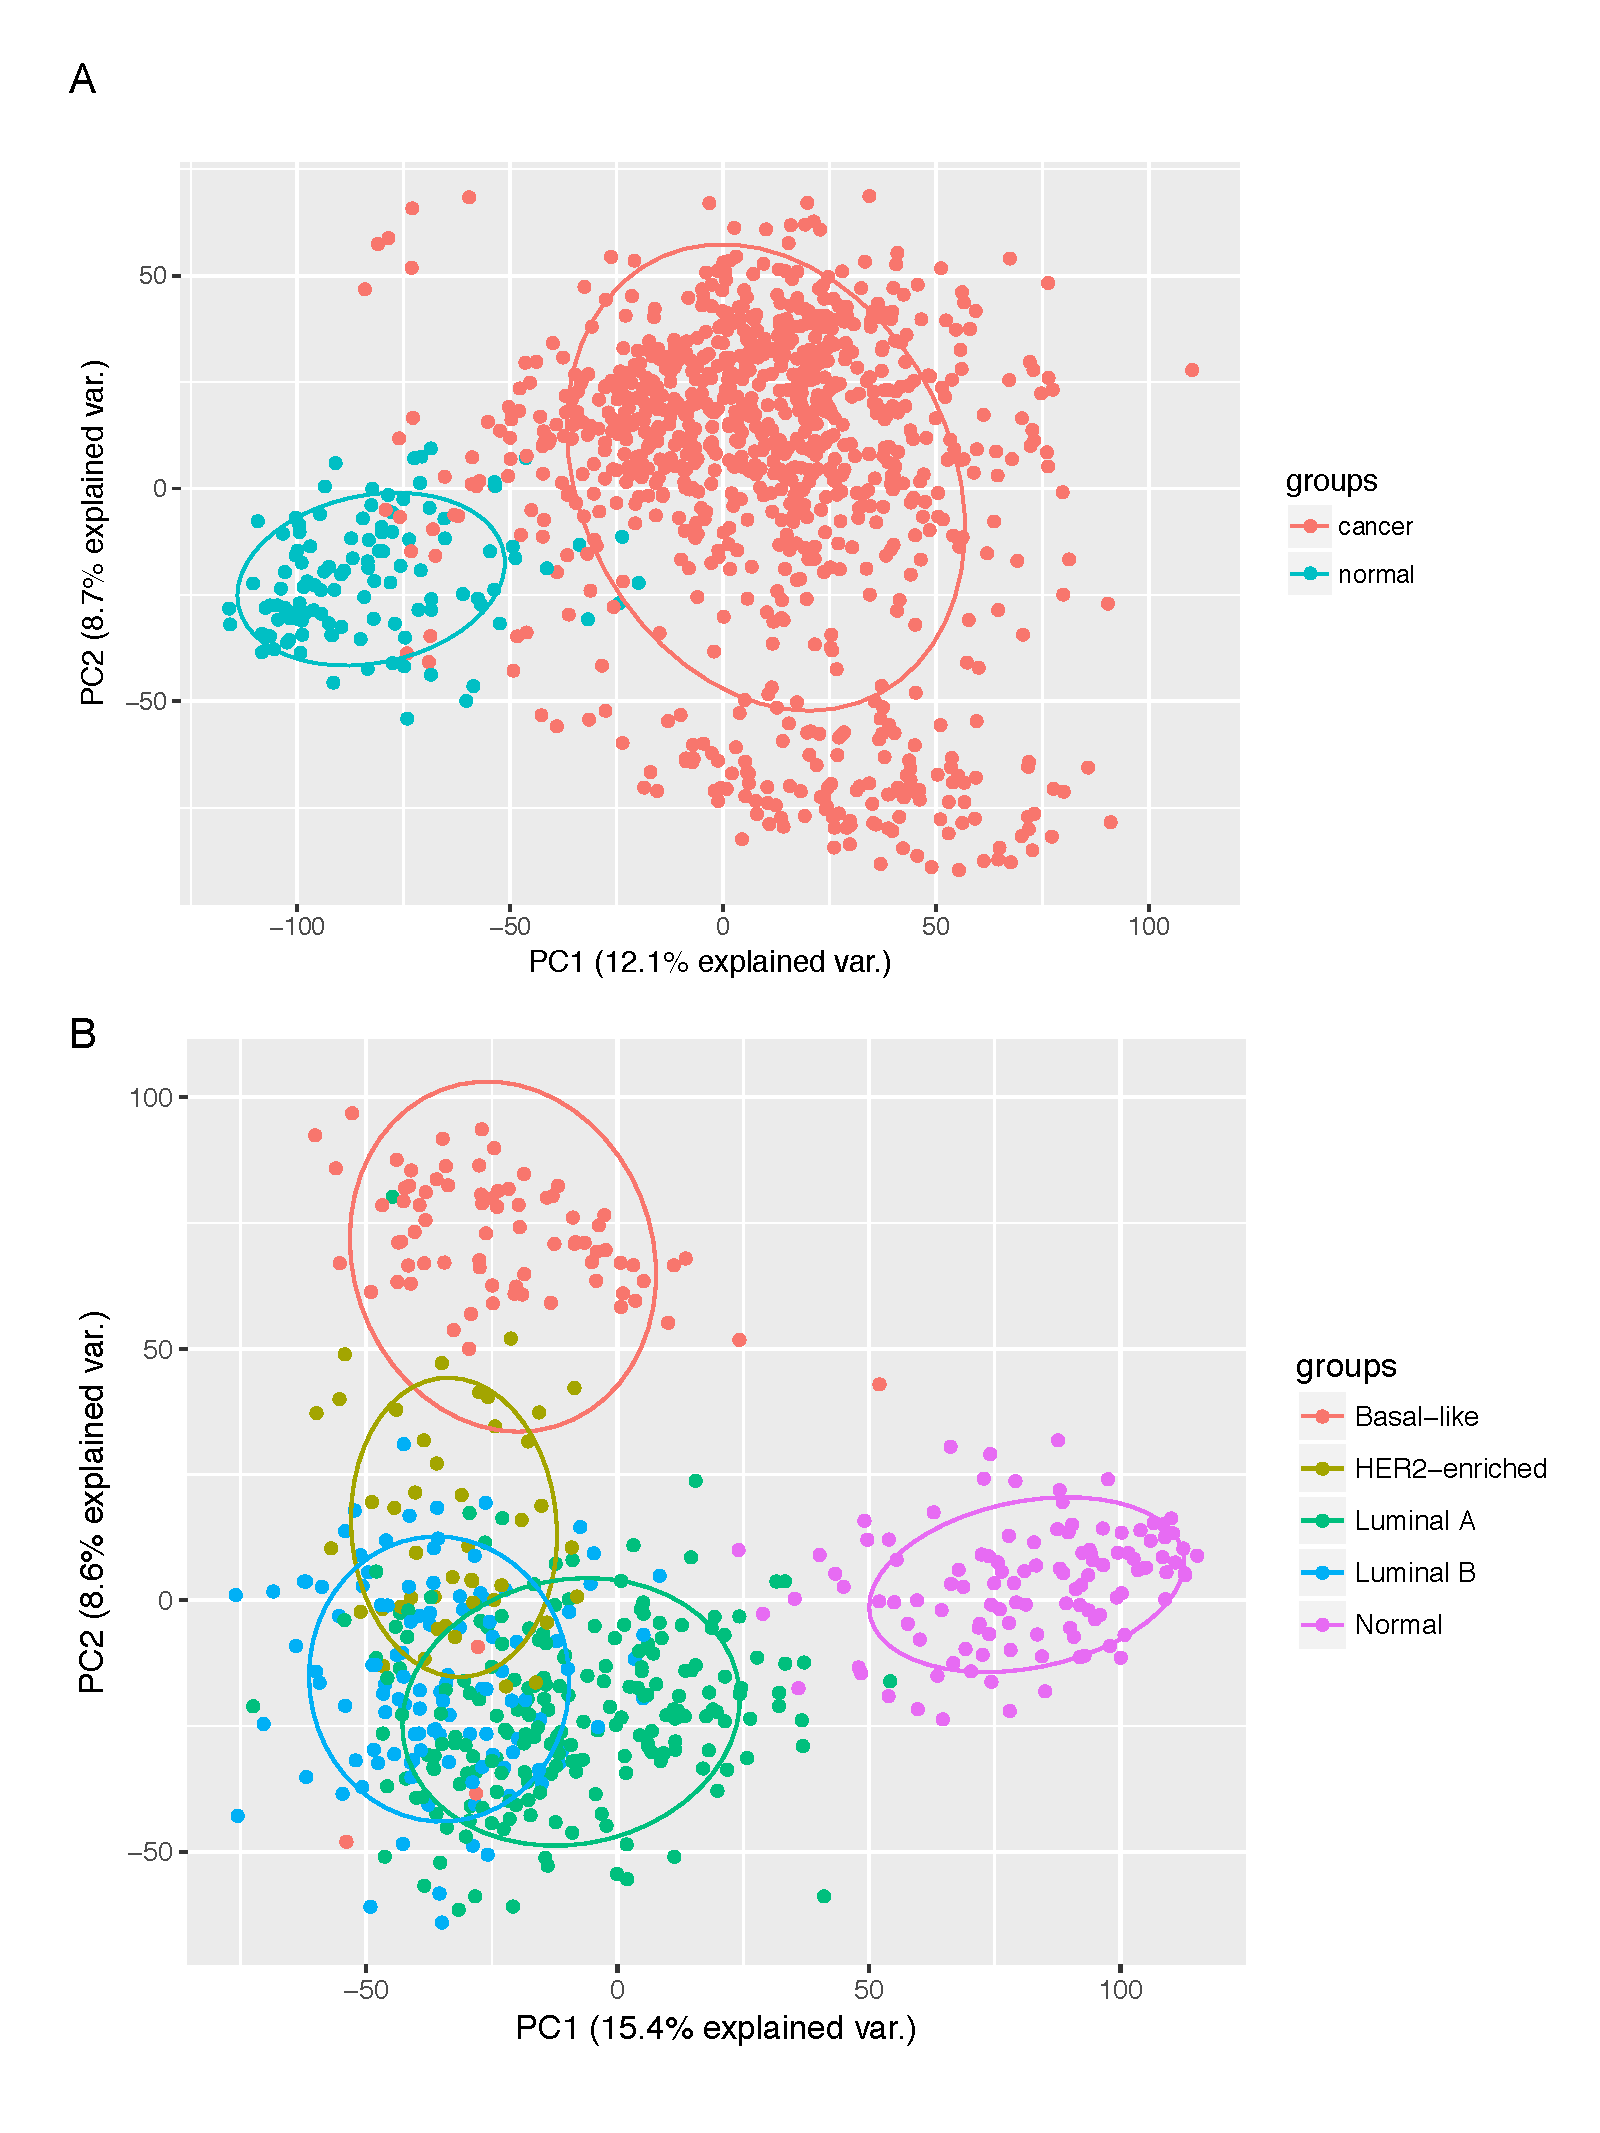
\includegraphics[width=\linewidth]{expl_pca.pdf}
\caption{{\bf PCA plot of transcriptional profiles of samples, stratified by tissue type and PAM50 'subtype's.}
A: PCA plot of the dataset after pre-processing. Color-coded according to tumor-adjacent normal tissue (normal) and tumor tissue (cancer). B: PCA plot of the dataset after pre-processing, limited to samples containing PAM50 subtype information. Color-coded according to subtype's: Basal-like, HER2-enriched, Luminal A, Luminal B, and Normal.}
\label{fig1}
\end{figure}


A critical part of a high-throughput study of a heterogeneous dataset such as the BRCA dataset, is the exploration of possible batch effects, contributing to the variation in gene expression between samples. Such effects may occur when measurements are affected by differences between experiments (e.g., date of experiments, operating technicians, instruments, and laboratory conditions). Batch effects may pose a serious challenge when confounded with an outcome of interest. In such cases, it may lead to decreased statistical power by adding possible unexplained variation, which may ultimately lead to incorrect conclusions~\cite{Leek2010, Liu2016}.
Many methods exist for the removal of batch effects, among which, methods applying two-way ANOVA or empirical Bayes statistics have been a popular choice in the scientific community. However, it has been demonstrated that for unbalanced data sets, these methods may systematically induce incorrect group differences and impact the reliability of downstream analysis~\cite{Nygaard2016, Liu2016}. Nygaard et al.~\cite{Nygaard2016} concluded from their study on effects that may arise from different batch adjustments methods, that the best approach was to account for batch effects in the model of the statistical analysis.

We carried out an exploratory analysis to identify possible sources of variation coming from non-biological sources (i.e., batches), by calculating PC of our dataset. Specifically, we plotted and compared the transcriptional profiles of the samples, stratified by variables that could be anticipated to be sources of technical variation: (i) the (sequencing) plate, (ii) the tissue source site (sequencing facility, tss), and (iii) the year the sample were processed (year). 

\smallskip

Fig~\ref{fig2} depicts a 2D scatter plot of the samples projected onto the first two PC's, with samples stratified according possible sources of variation. Samples were additionally projected onto PC 2-4 as well as 1D PCA plots in an effort to capture variation among the numerous subgroups. Ultimately, we omitted these results from the report, as they did not yield additional clarification. Moreover, we omitted the 2D scatter plot stratified by year, as it did not seem to describe any variation in the dataset.
In general, the numerous subgroups and large dataset makes it challenging to visually confirm patterns. Nevertheless, we suggest a correlation between the transciptional profiles and effects of tss and plate. 

Fig~\ref{fig2} A shows a pattern of samples deviating from the general trend, when stratified according to tss. We observe a pattern of samples in the right side (circle) originating from E9 (Asterand, color-coded pink), AC (International Genomics Consortium, color-coded darkgreen) and GI (ABS - IUPUI, color-coded pink). Looking into the dataset, we could see that all of these tss only sequenced normal tissue.
A similar situation is observed in Fig~\ref{fig2} B, showing a pattern of samples originating from plates, color-coded in blueish (A144, A14D, A14M, A157, A169). Again, we found that only normal tissue was sequenced in this plates.
Conclusively, a correlation seem to exist between the batch (tss and plate) and whether or not, the samples are from normal or tumor tissue. 
Based on these exploratory results, we opted to incorporate the effects of tss into the statistical analysis. We did not incorporate the effects of plate as we could see from the data, that the plates of interest were from the same tss. Thus, the tss was treated as a surrogate to avoid adding and extra parameter and associated degrees of freedom. Finally, we acknowledge that the first two PC's only retains 24\% of the original variances but as aforementioned, examining additional PC's, did not yield additional information when stratifying according to the variables under investigation here. As such, we would presumably need to include additional variables to clarify the remaining sources of variation.
\clearpage
\begin{figure}[hp!]
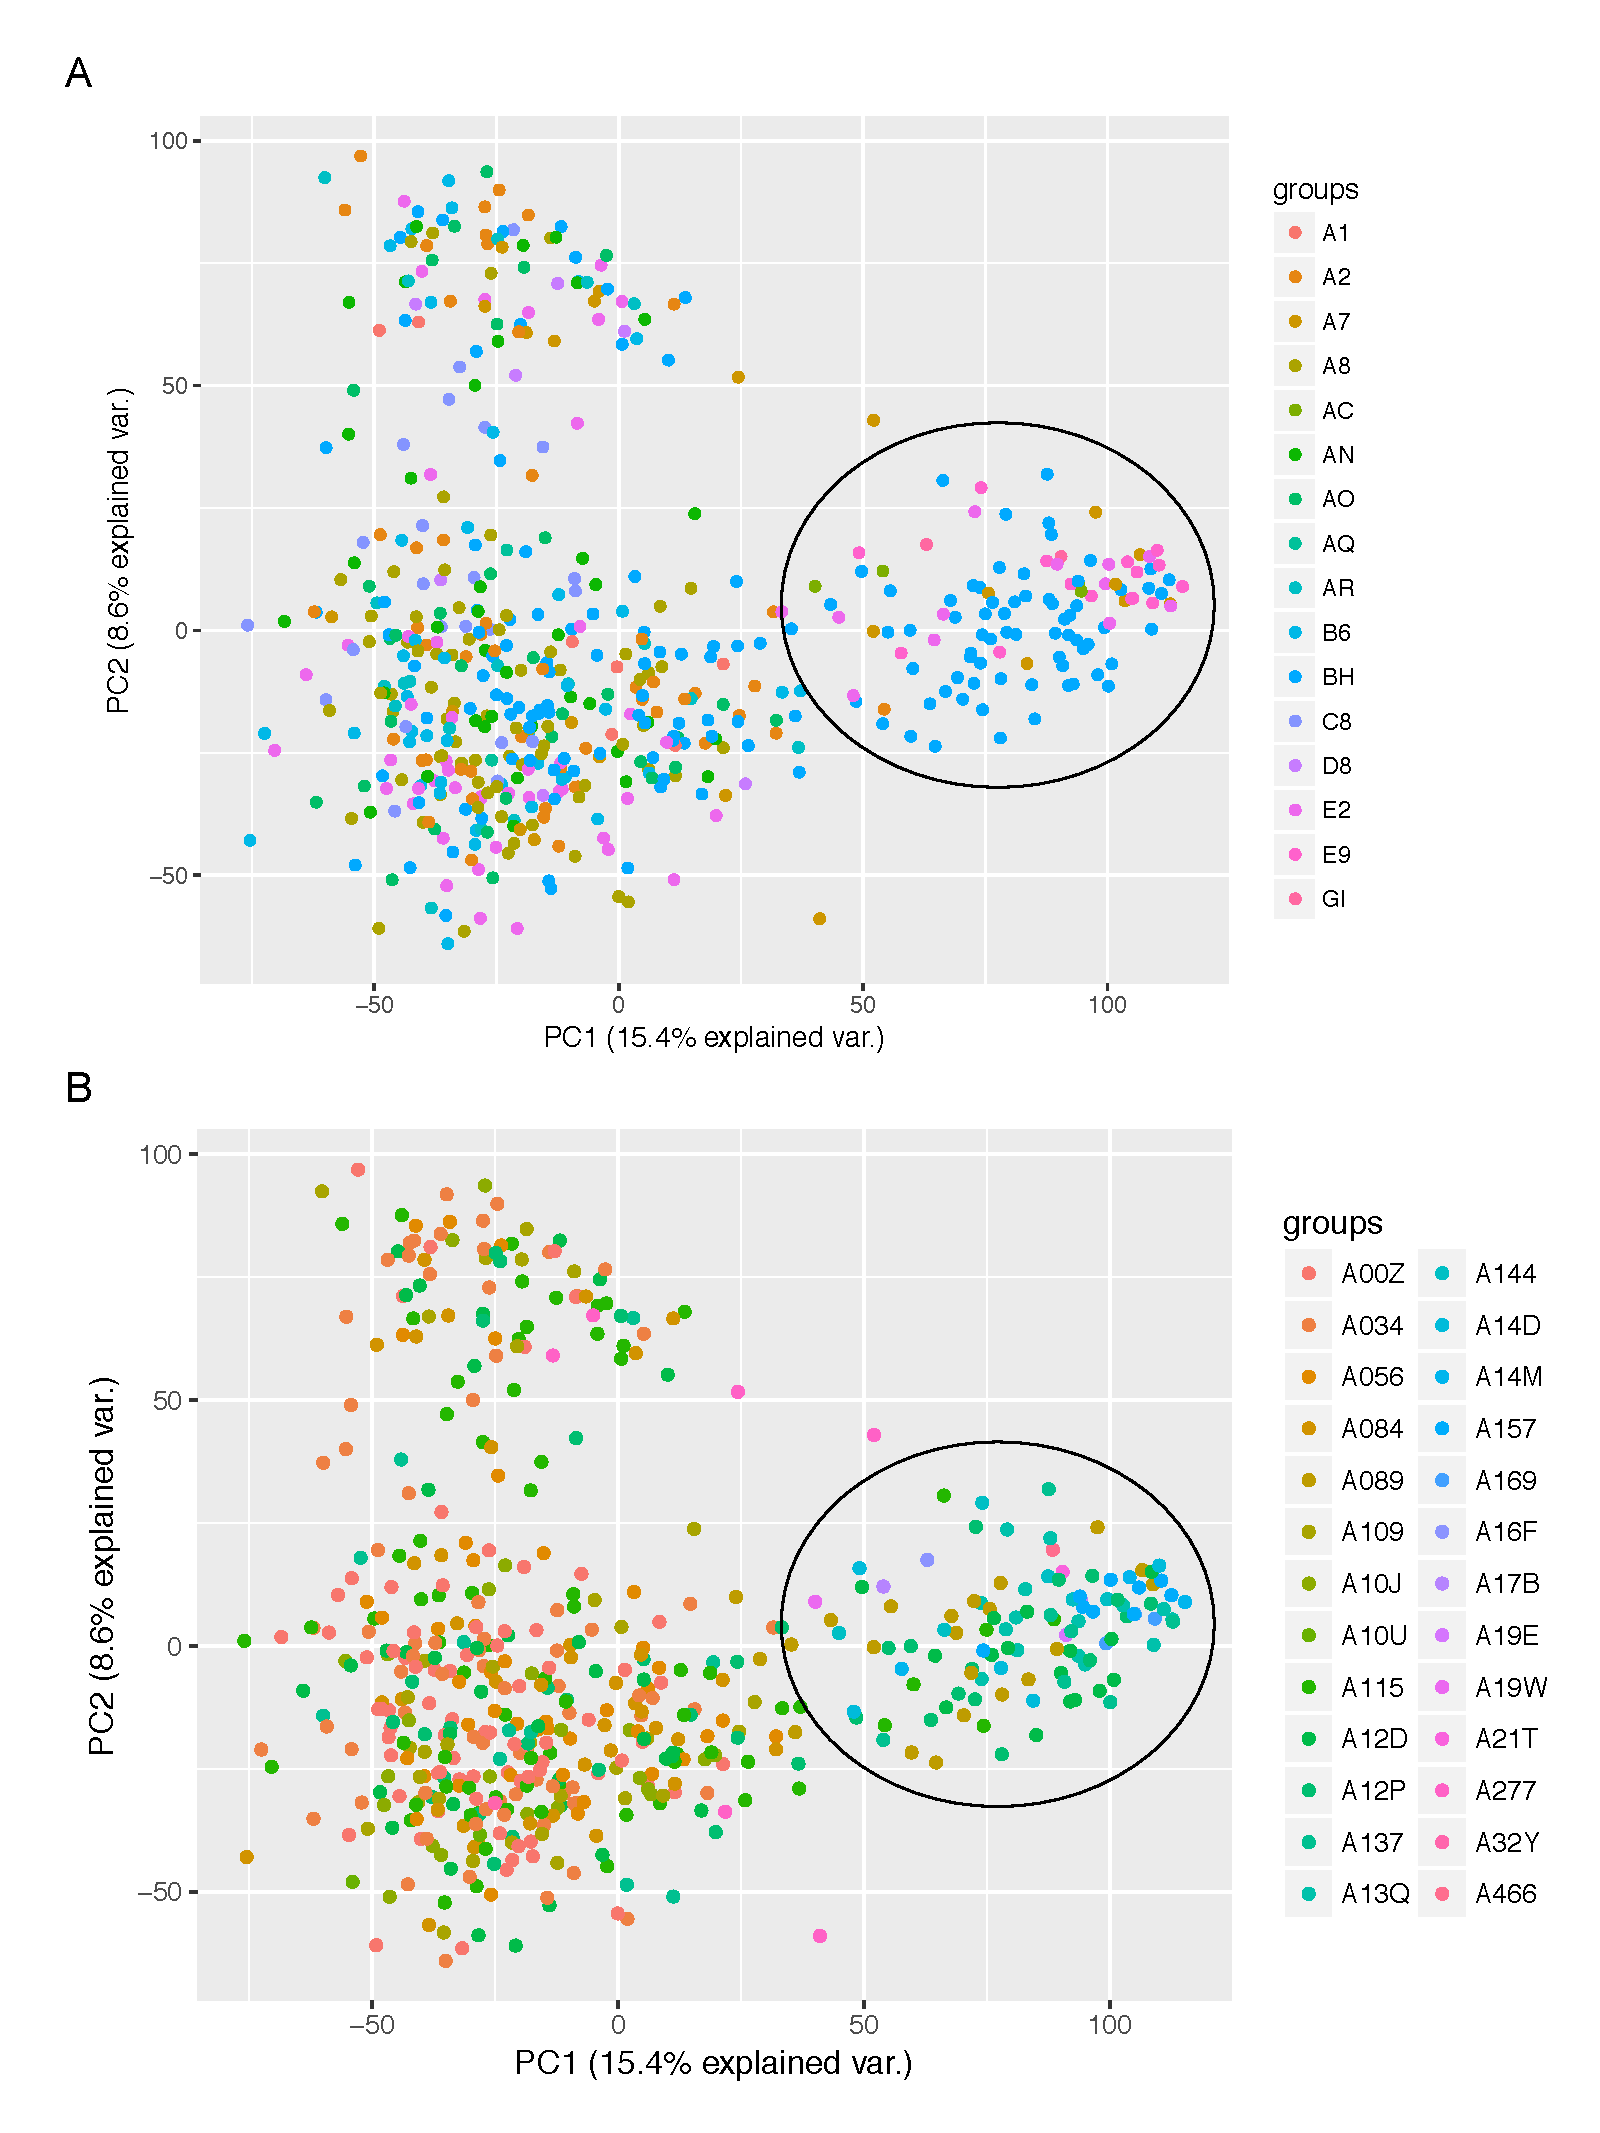
\includegraphics[width=\linewidth]{batch_expl.pdf}
\caption{{\bf PCA plot of transcriptional profiles of samples in the dataset, stratified by technical batches.}
PCA plot, color-coded according to A: tissue source site and B: plate. Circles indicates a number of batches that deviate from the general trend}
\label{fig2}
\end{figure}

\subsubsection*{Differential expression analysis}
Differential expression analysis (DEA) was performed on a final dataset, after pre-processing, normalization, and filtering, containing 14273 protein coding genes and 444 tumor samples, including subtype information (Luminal A, Luminal B, Basal-like, and HER2-enriched) and 113 tumor-adjacent normal tissues samples. The Normal-like subtype was filtered out as it only encompassed 4 samples.

To quantify the magnitude and significance of differential expression (DE) between the conditions, tumor and normal samples, we employed \textit{limma} - A well-developed framework for analyzing gene expression data integrating statistical methods for large-scale studies~\cite{Ritchie2015}.

\textit{limma} fits a gene-wise linear model to quantify DE, incorporating the statistic design (i.e., the conditions of interest and batch effects). Linear models assume the data to be approximately homoskedastic (i.e., approx. equal variance). Read counts generalized by RNA-seq experiments have noticeably unequal variance, with larger variances for larger counts. As a result, linear models would discriminate variances for smaller counts, and as such would predominantly depend on genes with high counts~\cite{Law2014}. To overcome this, we used the \textit{voom} function, converting the mean-variance trend into "precision weights", which can then be included into the linear model. Fig~\ref{fig3} depicts the mean-variance relationship of log-CPM expressions before and after \textit{voom} transformation. In compliance with \textit{voom} literature~\cite{Law2014}, we observed a decreasing log-CPM mean-variance trend (Fig~\ref{fig3} A), contrarily to the mean-variance trend of raw read counts. After \textit{voom} transformation (Fig~\ref{fig3} B), it is clear that the variation of the log-CPM becomes less dependent on the mean.
\clearpage
\begin{figure}[hp!]
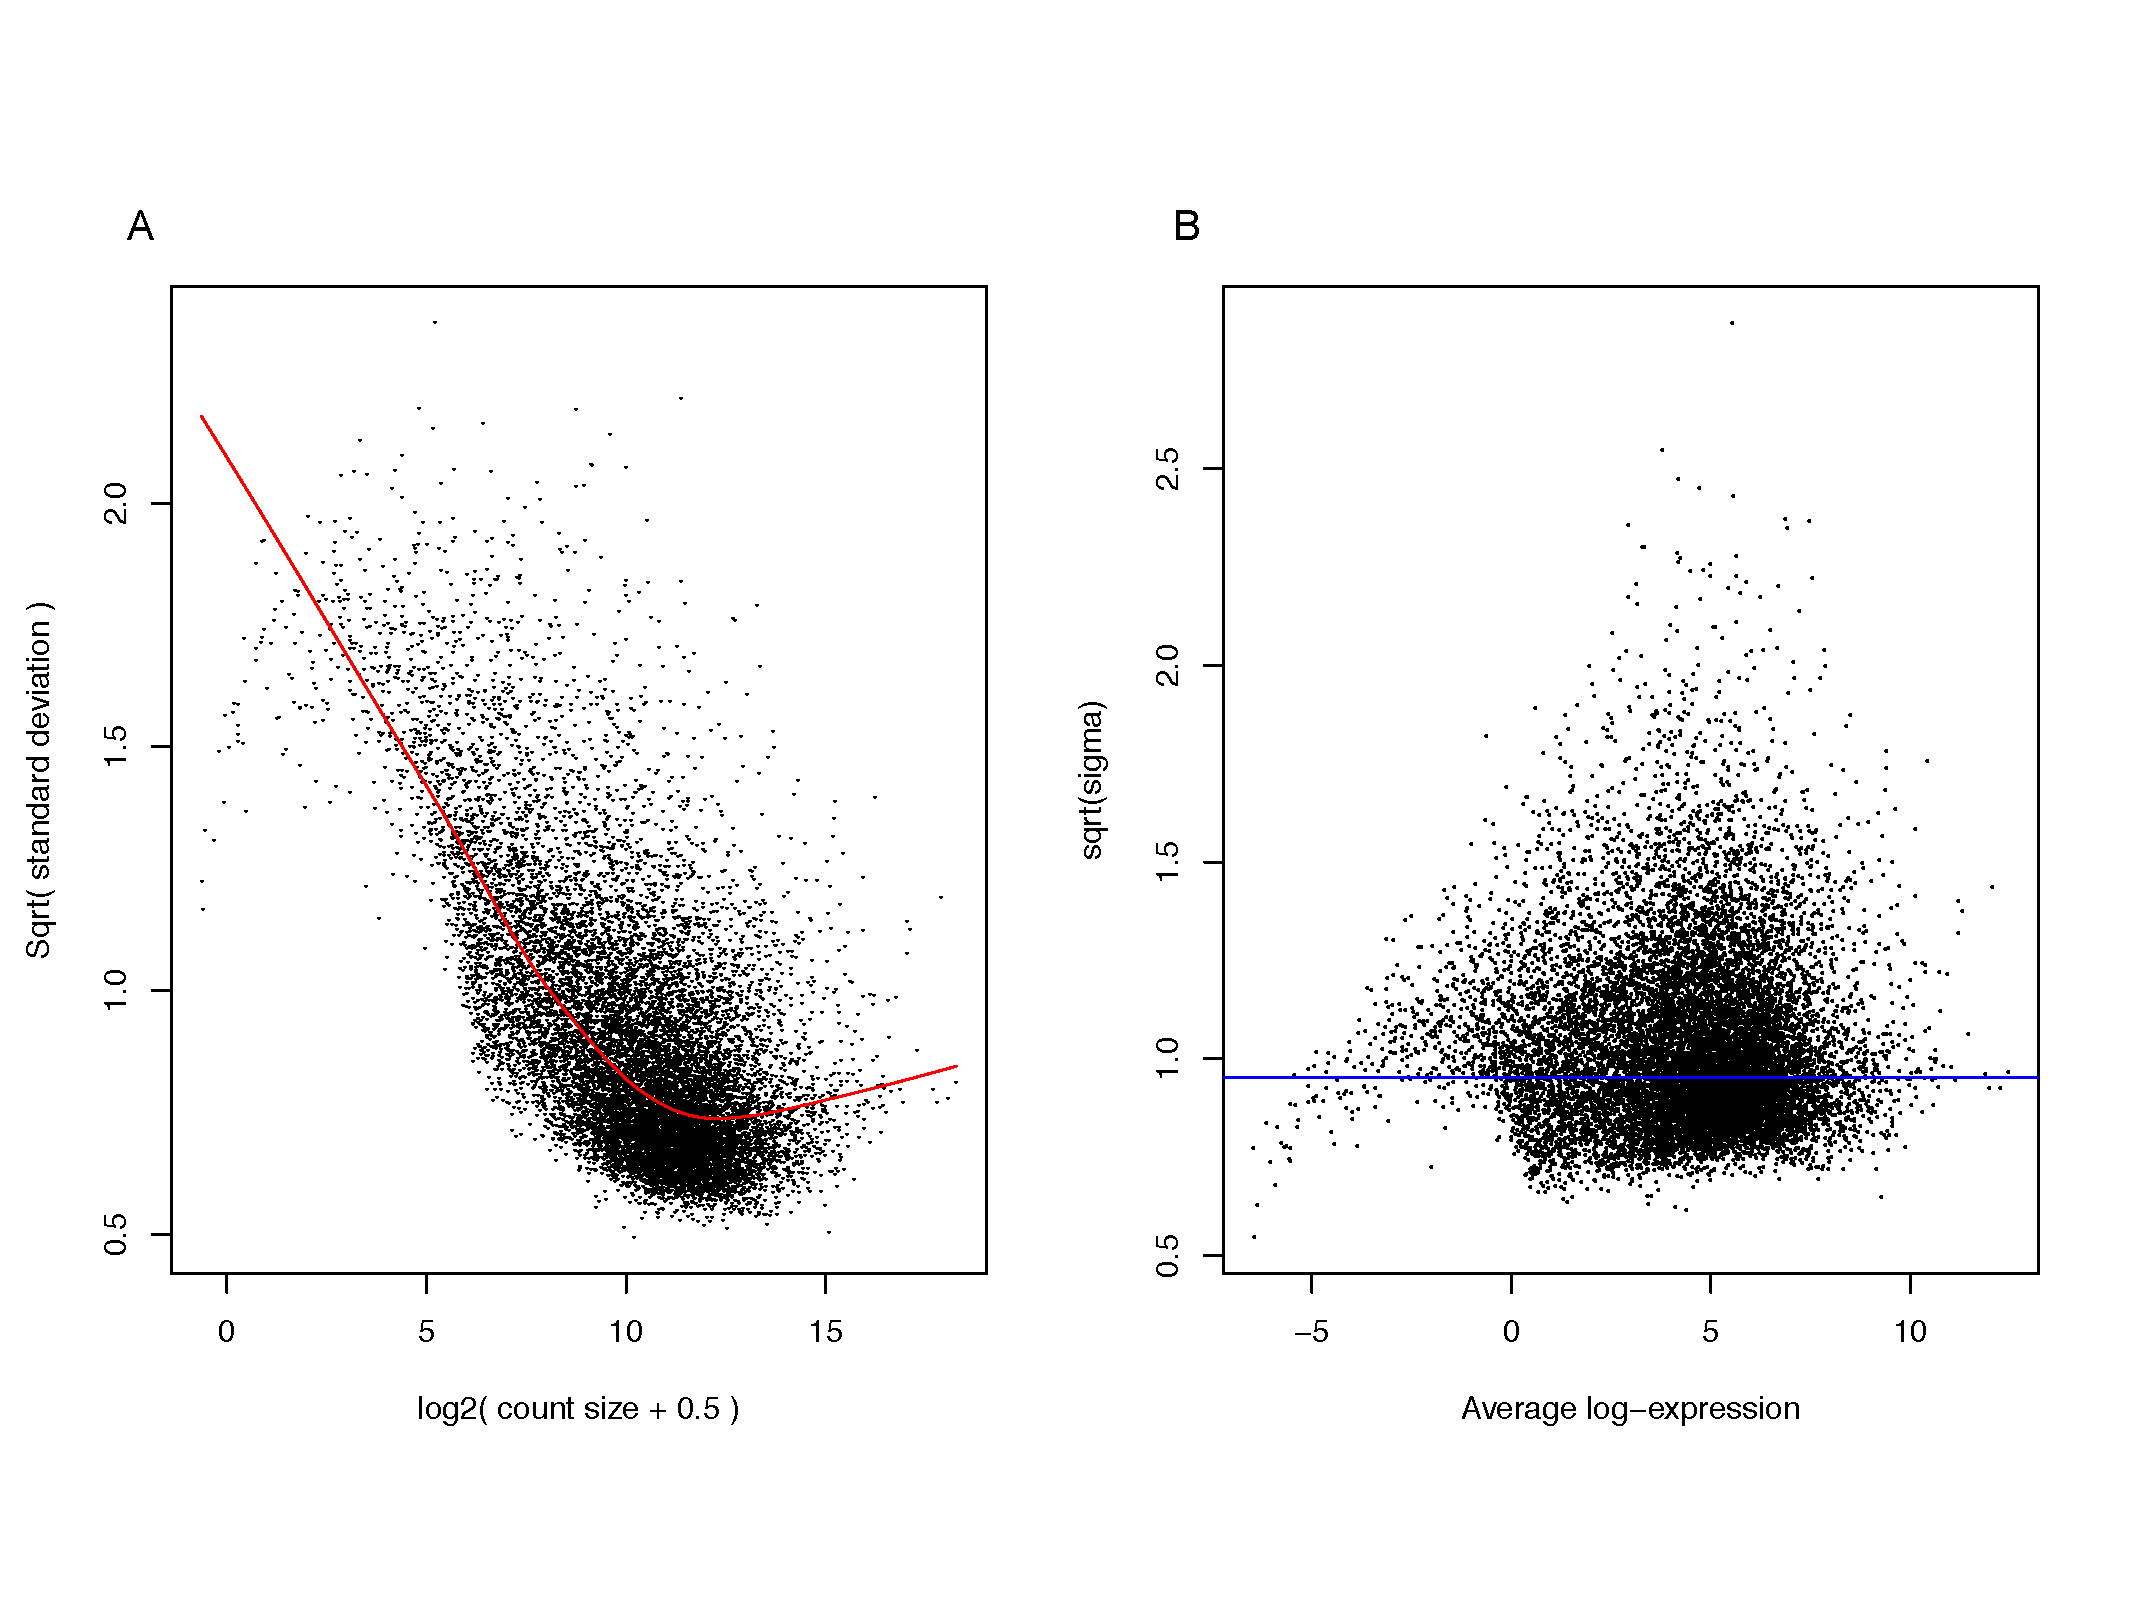
\includegraphics[width=\linewidth]{mean_variance.pdf}
\caption{{\bf Mean-variance relationship of log-CPM values.}
A: Before \textit{voom} transformation. $Log_{2}$ transformed means with an offset of 0.5 (x-axis) are plotted against the variance (y-axis), rescaled to square-root of standard deviations. B: After \textit{voom} transformation. $Log_{2}$, residual standard deviations (y-axis) are plotted against mean log-CPM values (x-axis).}
\label{fig3}
\end{figure}

A log-fold-change (logFC) of 1 was applied as a threshold for determining DE between the two conditions, and significance was defined using an fdr adjusted p-value \textless 0.05. 3092 genes were found differentially expressed, 1738 downregulated and 1354 upregulated in tumor tissue compared to normal tissue. 45 candidate genes were differentially expressed with 21 genes, upregulated and 24 genes, downregulated. To assess the similarity of gene expression patterns between candidate genes in the two conditions, we performed unsupervised clustering. From the heatmap, it is clear that the pattern of gene expressions between the tumor (cancer) and normal is distinct and clusters well between the conditions. For more information, see \nameref{S2_Fig} Supporting information.

\smallskip

Magnitude and significance of gene expressions were summarized in a volcano plot and the 45 candidate genes highlighted (Fig~\ref{fig4}).   
\clearpage
\begin{figure}[h!]
% 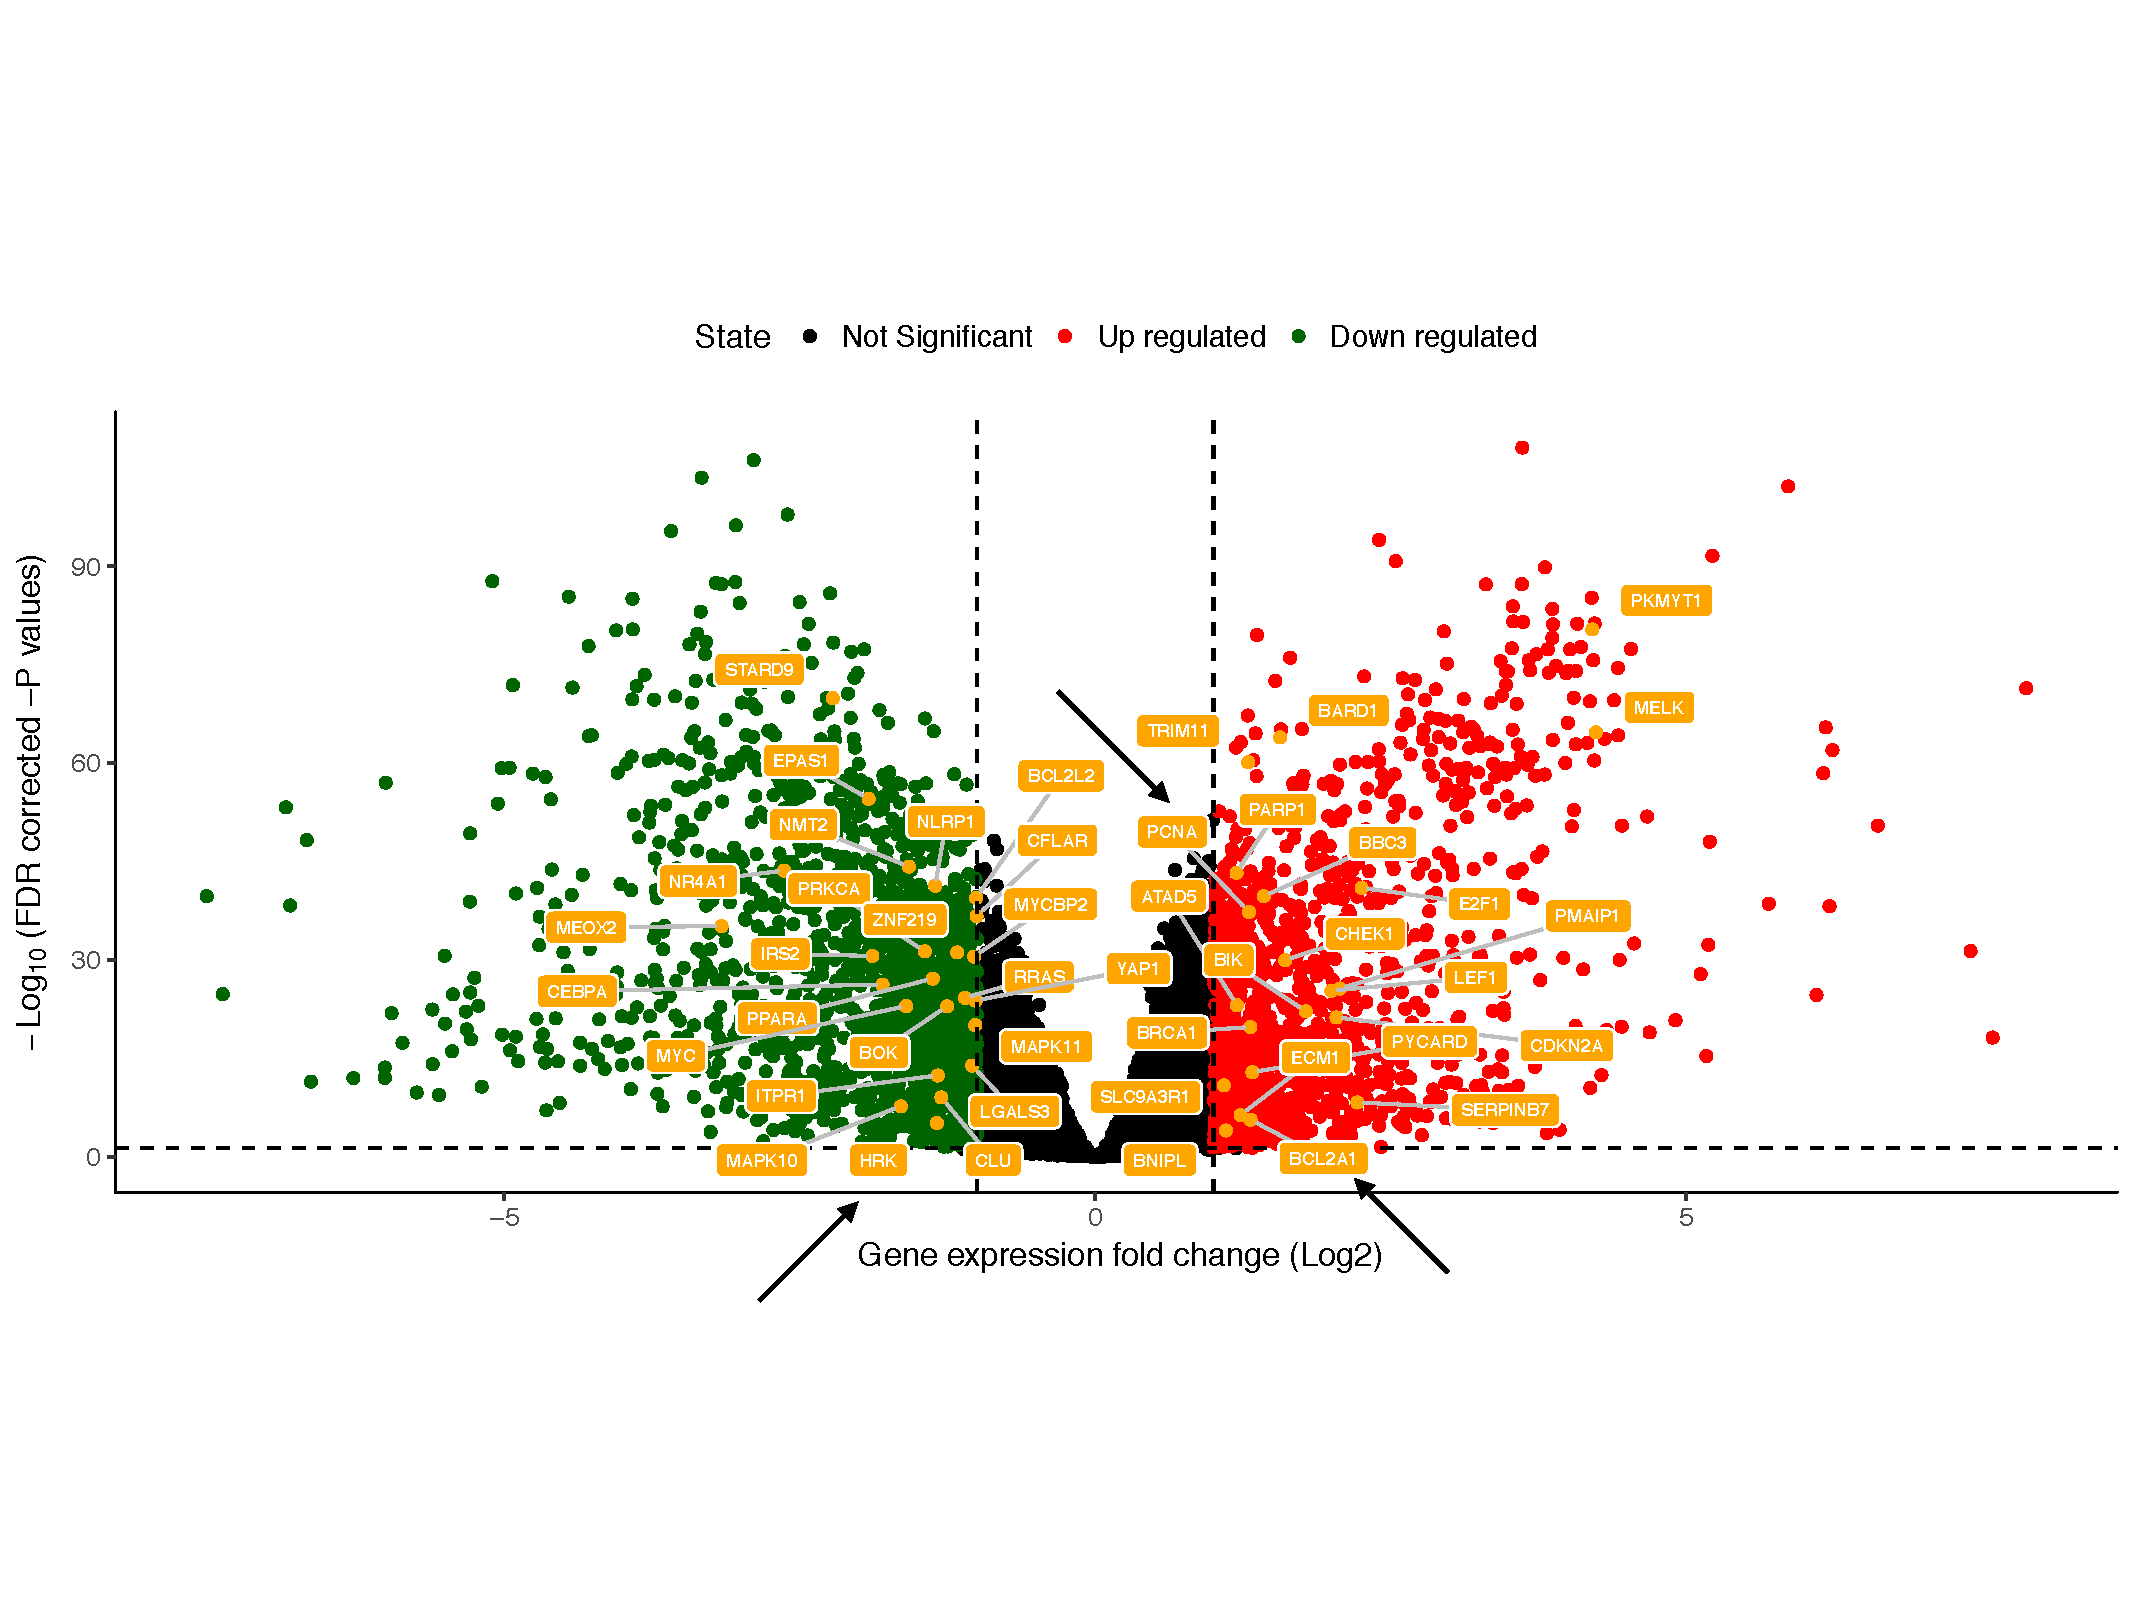
\includegraphics[width=\linewidth]{volcano.pdf}
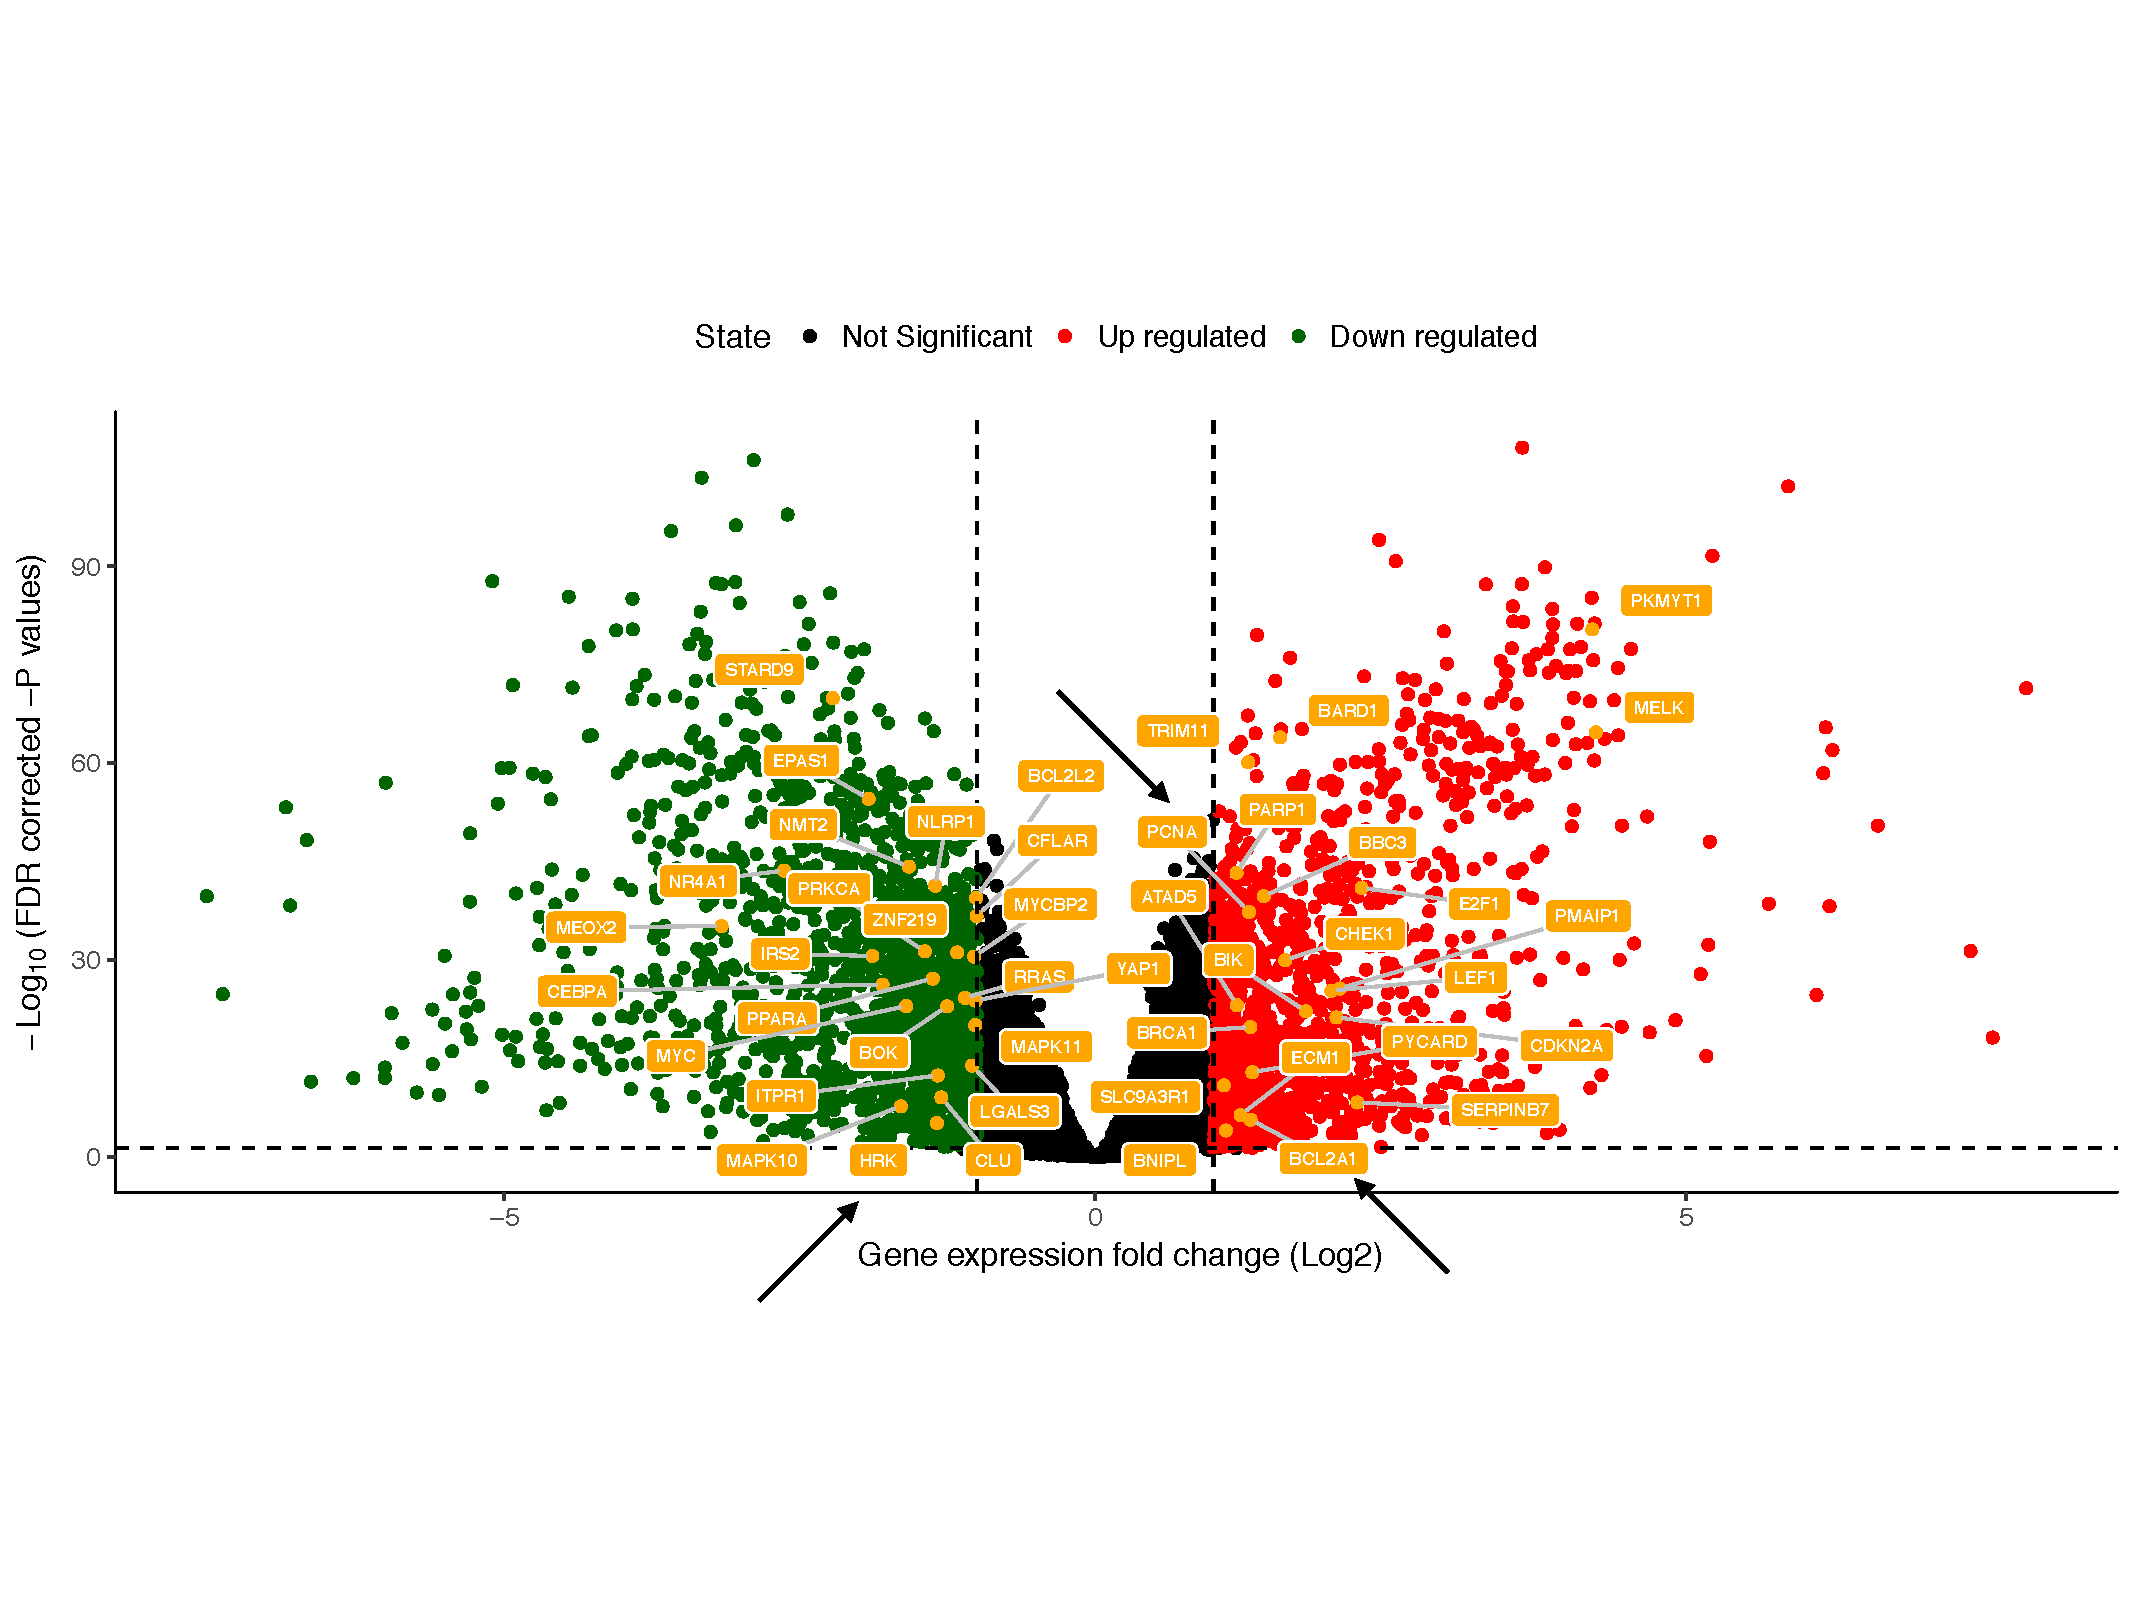
\includegraphics[width=1.4\textwidth,right]{volcano.pdf}%

\caption{{\bf Volcano plot representation of DE between tumor and normal tissue.}
$-Log_{10}$ transformed adjusted p-values are plotted against the gene expression magnitude in terms of logFC. Differentially expressed candidate genes are highlighted with labels. The horizontal dashed line shows the adjusted p-value cutofff (0.05) with dots above the line having p-value \textless 0.05. The vertical dashed line shows the logFC with genes to the left being downregulated and genes to the right, upregulated. Arrows indicates genes of interest.}
\label{fig4}
\end{figure}

For the purpose of this study, we chose to focus our attention on a limited number of deregulated genes. More precisely, we chose Bcl2a1, encoding the pro-survival Bcl-2 member, Bcl-2-related protein A1, and the two genes Hrk, encoding Activator of apoptosis harakiri and Pcna, encoding Proliferating cell nuclear antigen. Bcl2a1 (logFC=1.31 and p.adj=2.4e-06) and Pcna (logFC=1.30 and p.adj=5.3e-38) were found to be upregulated in tumor versus normal, while Hrk (logFC = -1.34 and p.adj = 7.5e-06) were downregulated in the comparison.

\smallskip

A gene co-expression network can be used to identify genes that tends to show a coordinated expression pattern across samples. Co-expressed genes are likely controlled by the same transcriptional regulatory program, functionally related, or take part in the same pathways. Therefore, gene co-expression network can be used to relate genes of unknown function with biological processes~\cite{VanDam2017}. We carried out a gene co-expression network of \textit{voom} transformed expression values for the candidate genes, with the aim of identifying co-expression patterns between globular Bcl-2 members and putative BH3-like interactors (Fig~\ref{fig5}). 
\clearpage
\begin{figure}[hp!]
% 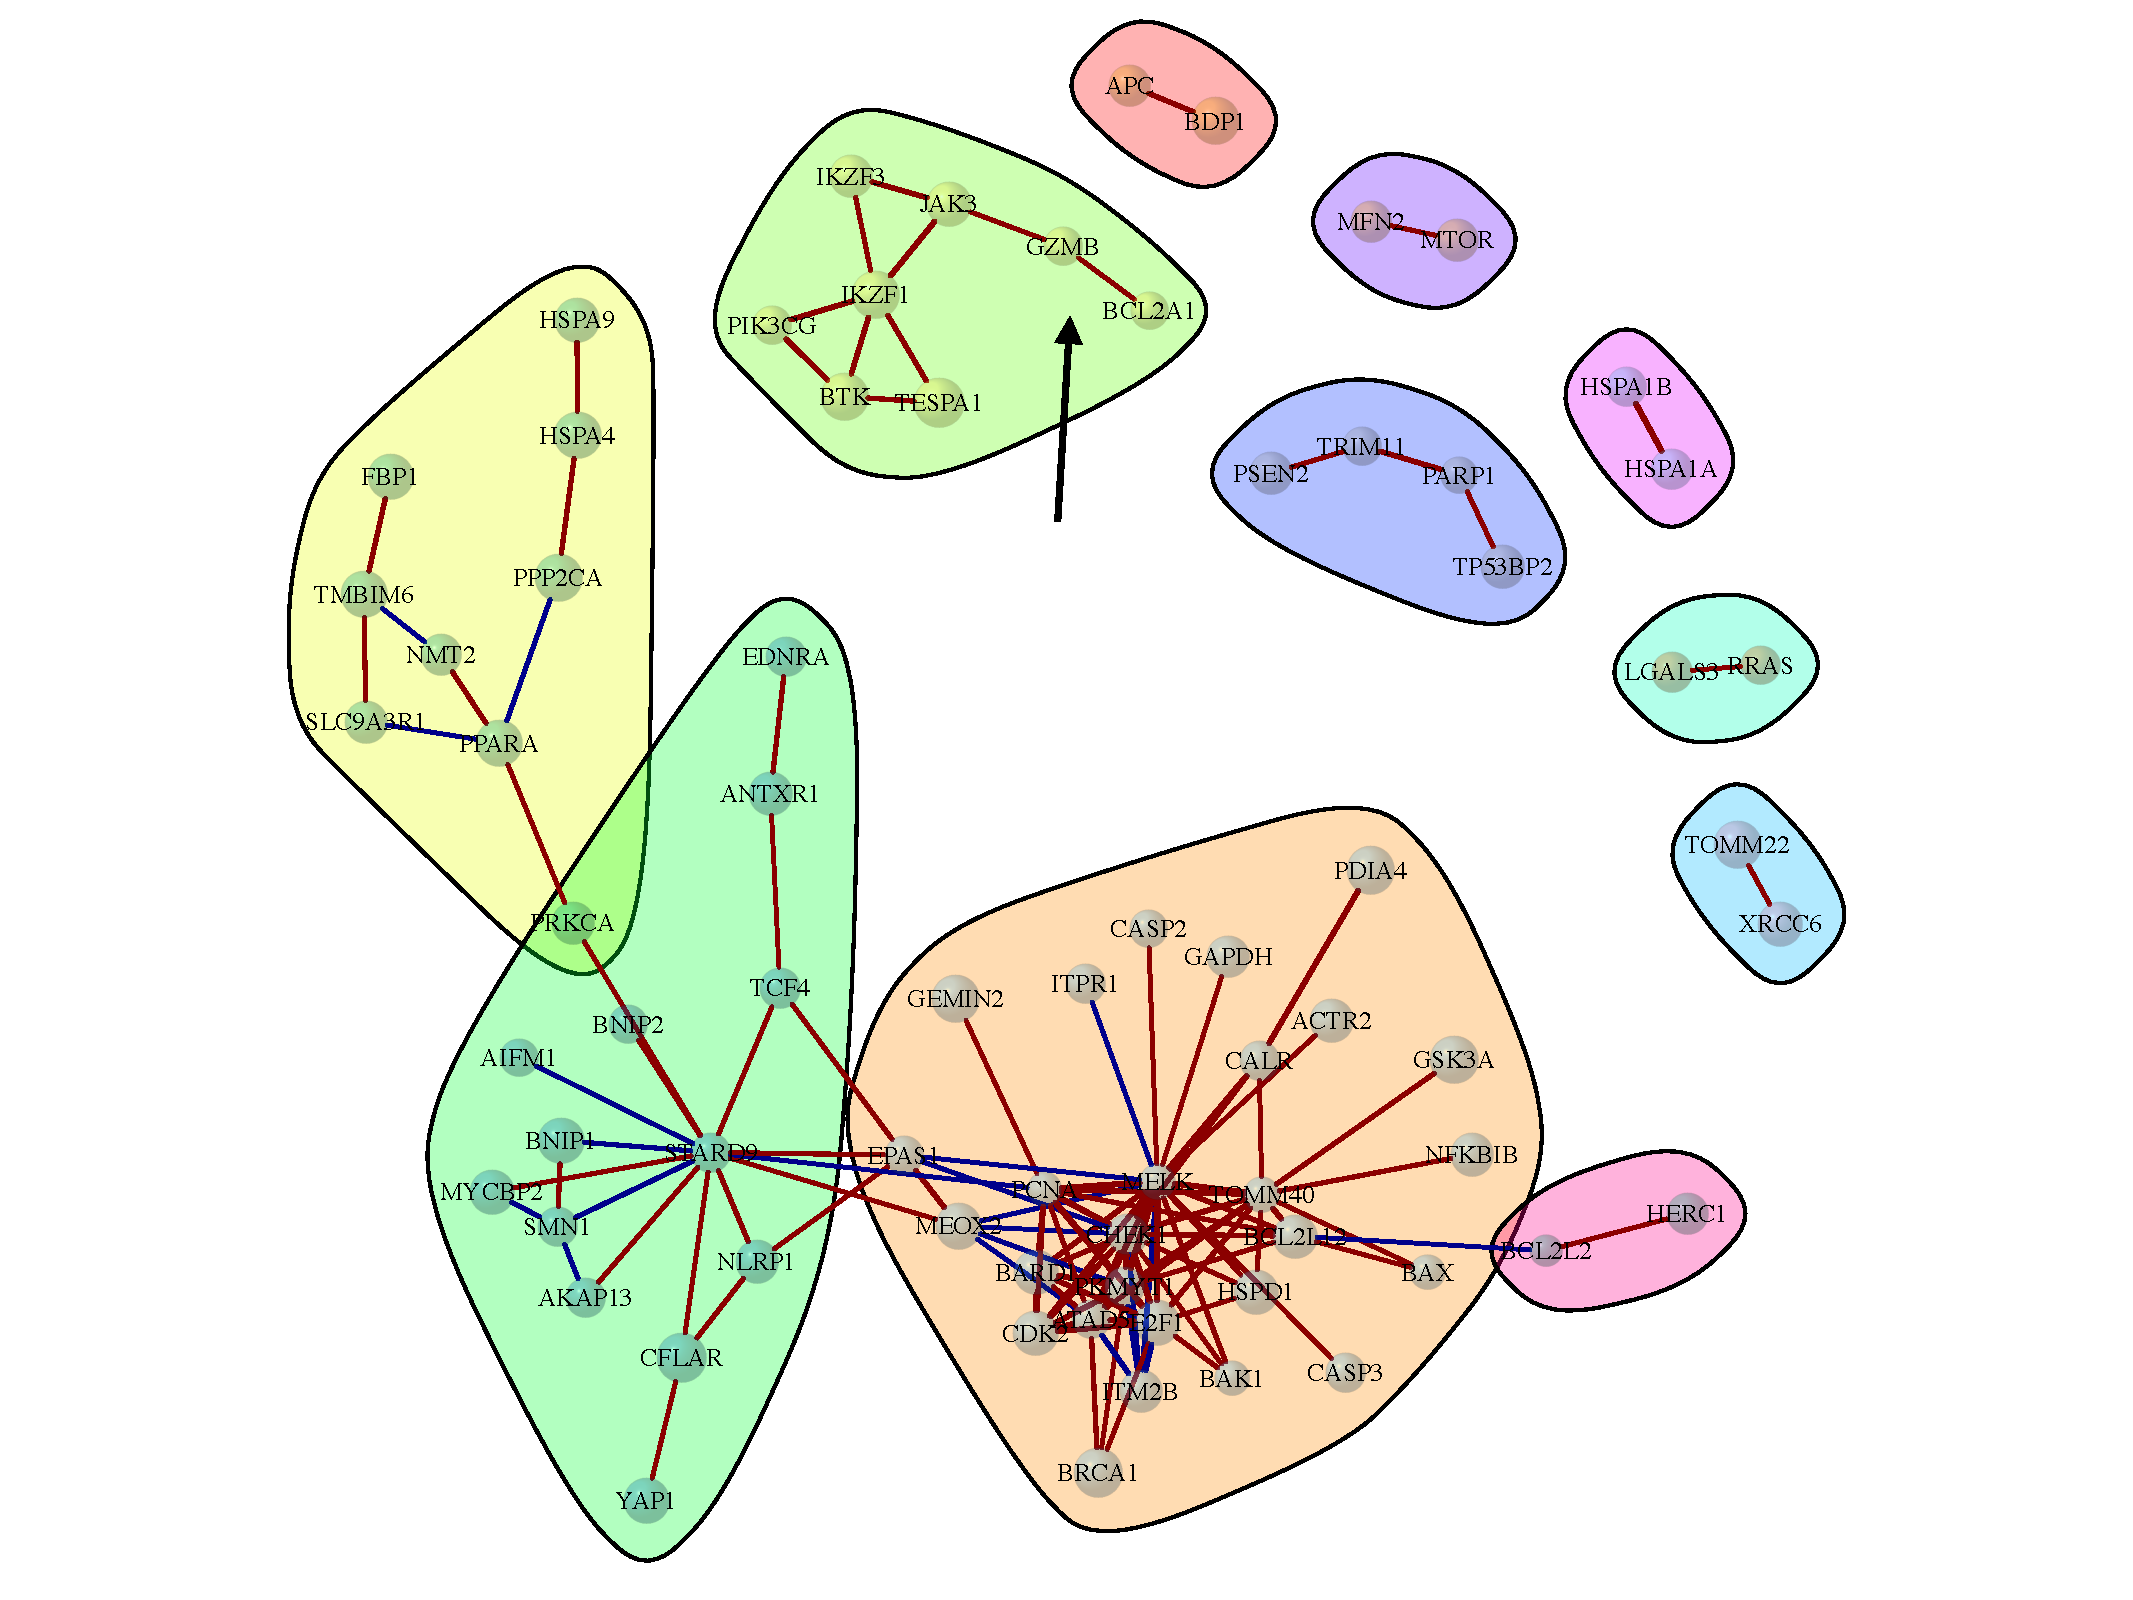
\includegraphics[width=\linewidth]{co_exp_net.pdf}
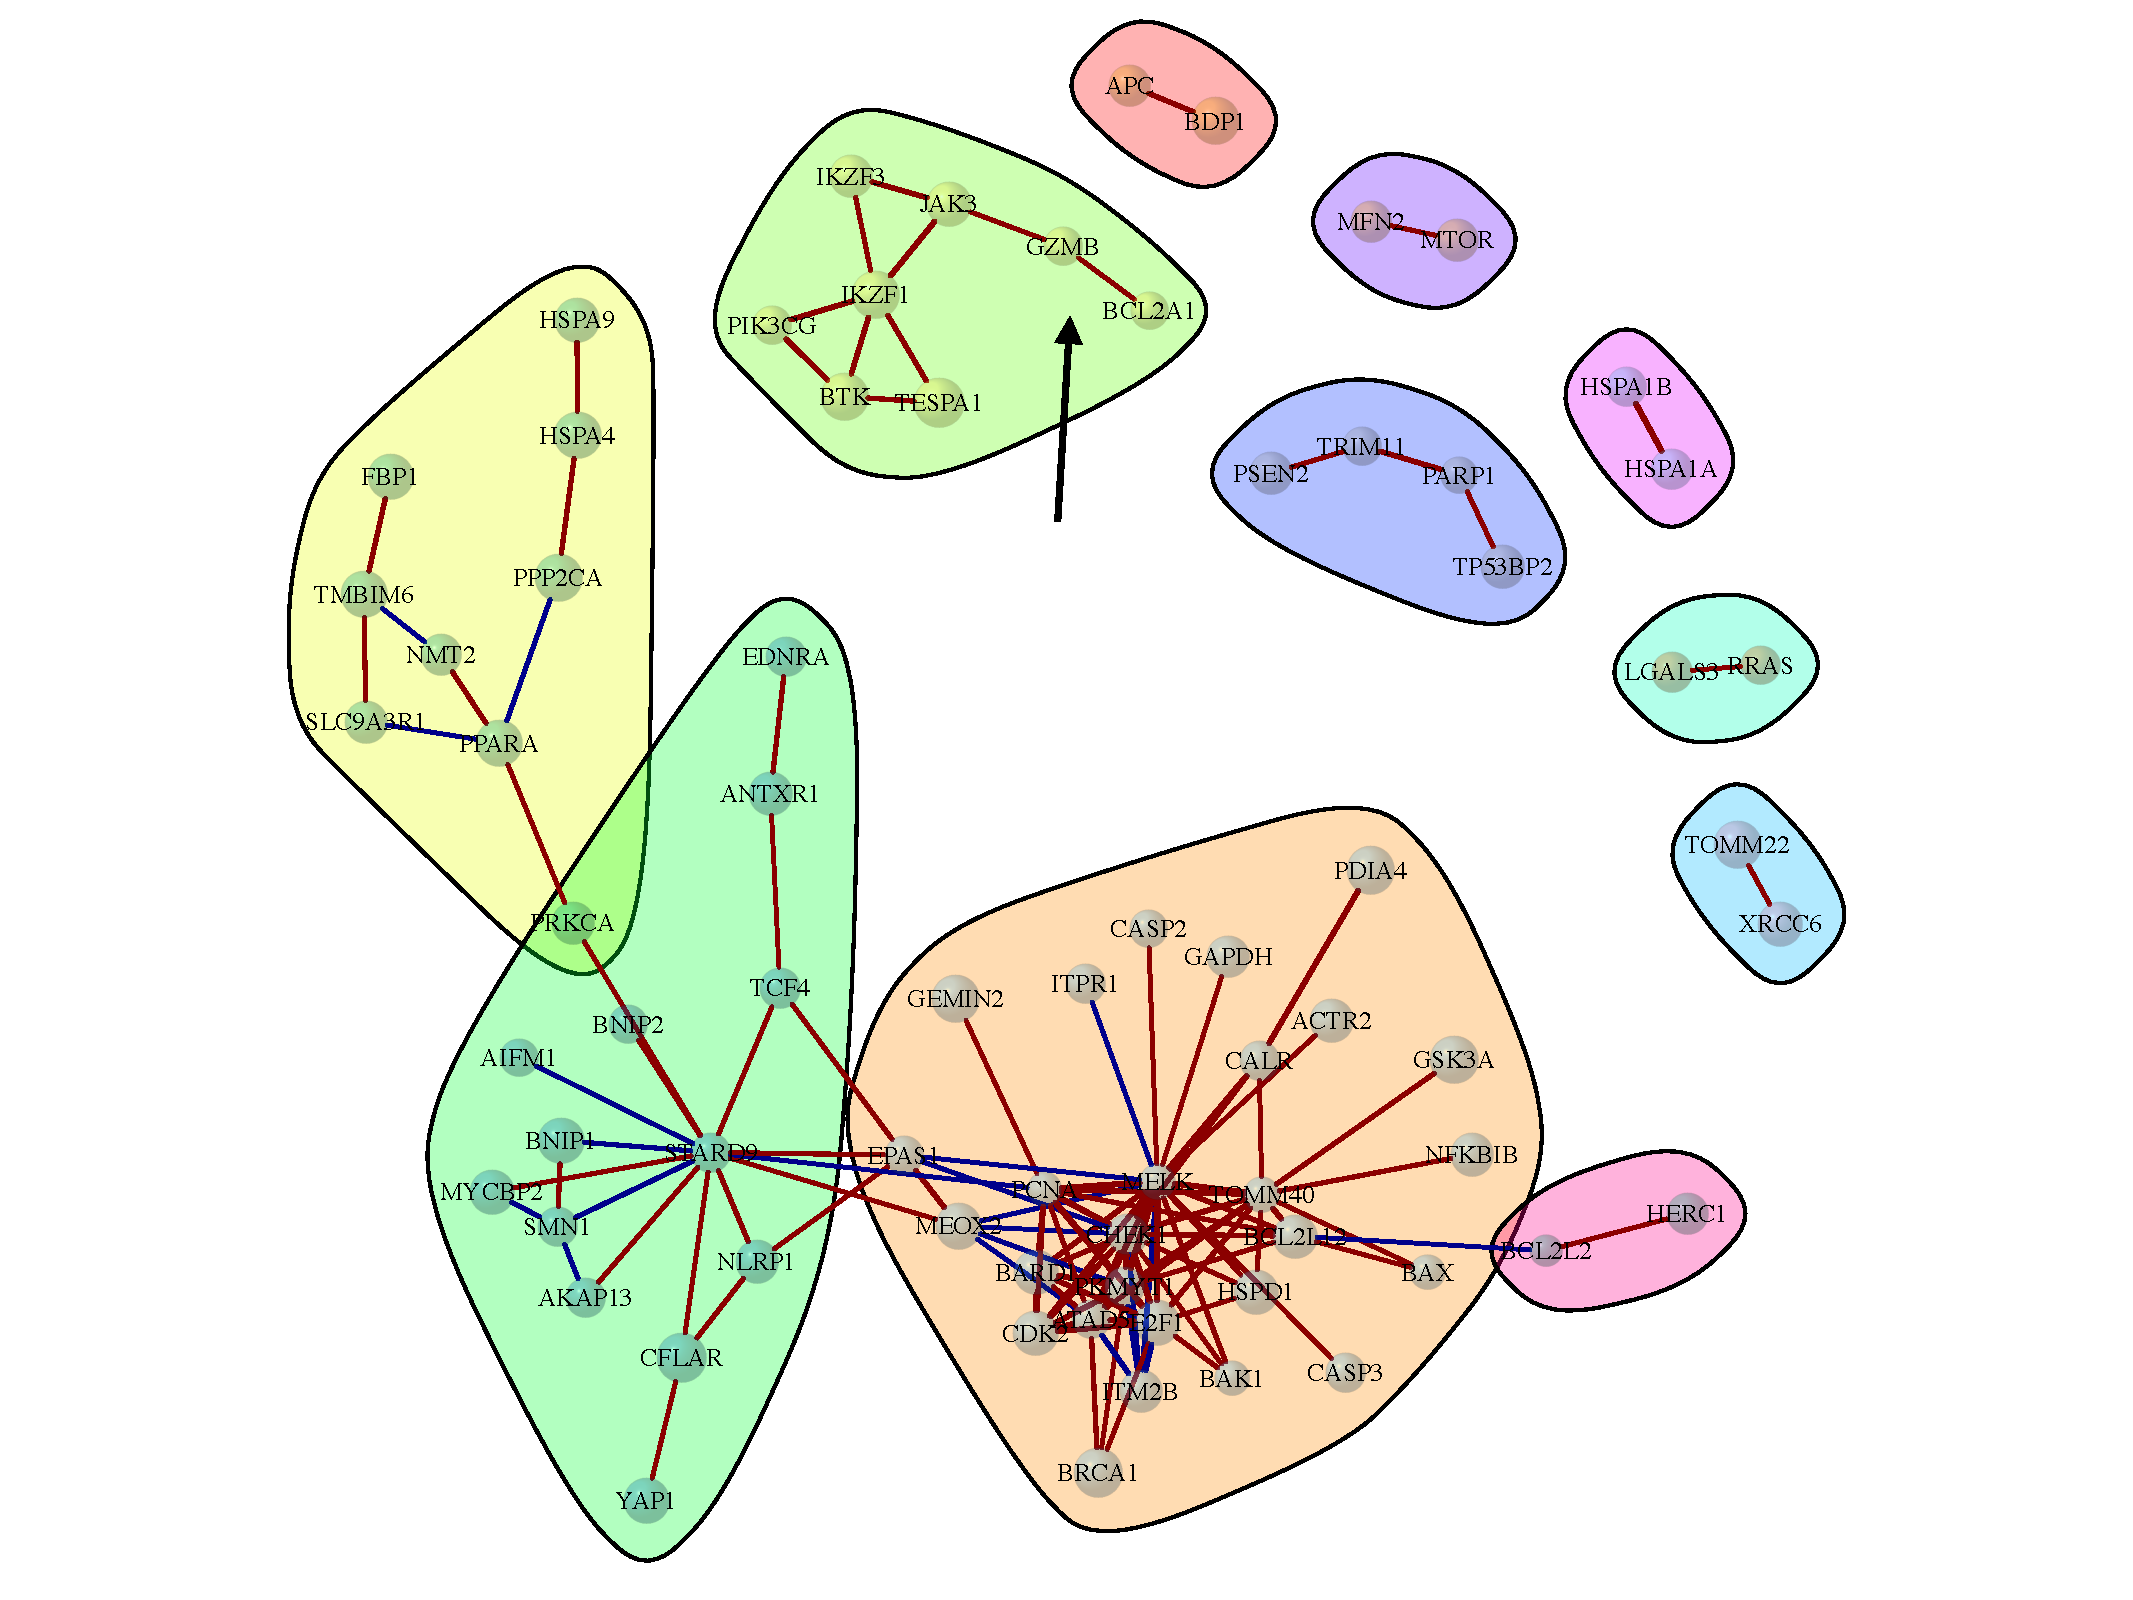
\includegraphics[width=1.4\textwidth,right]{co_exp_net.pdf}%

\caption{{\bf Gene co-expression network of candidate genes.}
Clustering of significantly (adj.p \textless 0.05) co-expressed genes. Edges are colored according to directions of correlation: Red, positive correlated; Blue, negatively correlated. Candidate Gzmb, indicated by arrow.}
\label{fig5}
\end{figure}

Fig~\ref{fig5} depicts clusters of co-expressed candidate genes. We have identified Bcl2a1 as a gene of interest and are predominately interested in interactors showing a co-expressed pattern with Bcl2a1, indicating that they could be part of the same biological processes. From the network, we identified the Bcl2a1 co-expressed gene Gzmb, encoding the protein Granzyme B. 

\smallskip

In the following, we will zoom in on the structural level of the proteins encoded by Bcl2a1, Hrk, Pcna, and Gzmb, using molecular modelling and \textit{in silico} mutagenesis.

\subsection*{Comparative modelling of protein-peptide complexes}
Comparative modelling, also known as homology modelling, is a model building approach in which a three-dimensional model of a target protein of unknown structure is modelled on the basis of a known three-dimensional template structure of a homologous protein. It relies on the fact, that structures of homologous proteins are more conserved than their sequences throughout evolution and as such, proteins with similar sequences adopt similar three-dimensional structure. As a result, structural similarity can to a large extent, be presumed if sequence similarity between two proteins is prevalent~\cite{Lesk1980,Marti-Renom2000}.

We employed \textit{MODELLER} to model protein-peptide complexes between Bcl2a1 and the four putative BH3-like interactors with the scope of predicting the three-dimensional structure and binding interface. The peptides includes: Hrk-28\_50, Hrk-63\_85 (two regions in Hrk, matched our BH3 motif search), Pcna-142\_164, and Gzmb-118\_140, denominated by protein name and location of putative BH3 motif. 

The quality of a predicted model is very much related to the sequence identity. When the sequence identity between the target and template is above 50\% and the protein is larger than 60 amino acids, the quality of the model is usually very high. When modelling smaller free-state peptides (\textless 30 amino acids), the quality declines and caution should be made. Modelling smaller peptides as part of a complex, increases the quality as the binding environment will put additional restraints on the peptide~\cite{zvelebil2008}. We are modelling our complexes against a experimentally derived complex containing the same protein (Bcl2a1) and a peptide with a similar motif. As a result, we are assuming our peptides to interact in a similar manner in the binding interface and are thus confident in the reliability of the models.  

\smallskip

Comparing our modelled complexes to the known structure of the canonical BH3-only peptide Puma, complexed with the pro-survival Bcl2a1, permit us to investigate if the putative BH3 peptides have the properties an structural features of a canonical BH3-only peptide. 

We visually inspected our model to assure, that the key binding residues were correctly facing towards the binding interface and compared locations of these key residues to the canonical BH3-only peptide Puma (Fig~\ref{fig6}). Moreover, we assessed that the modelled core confirmed to general structural rules.

\begin{figure}[hp!]
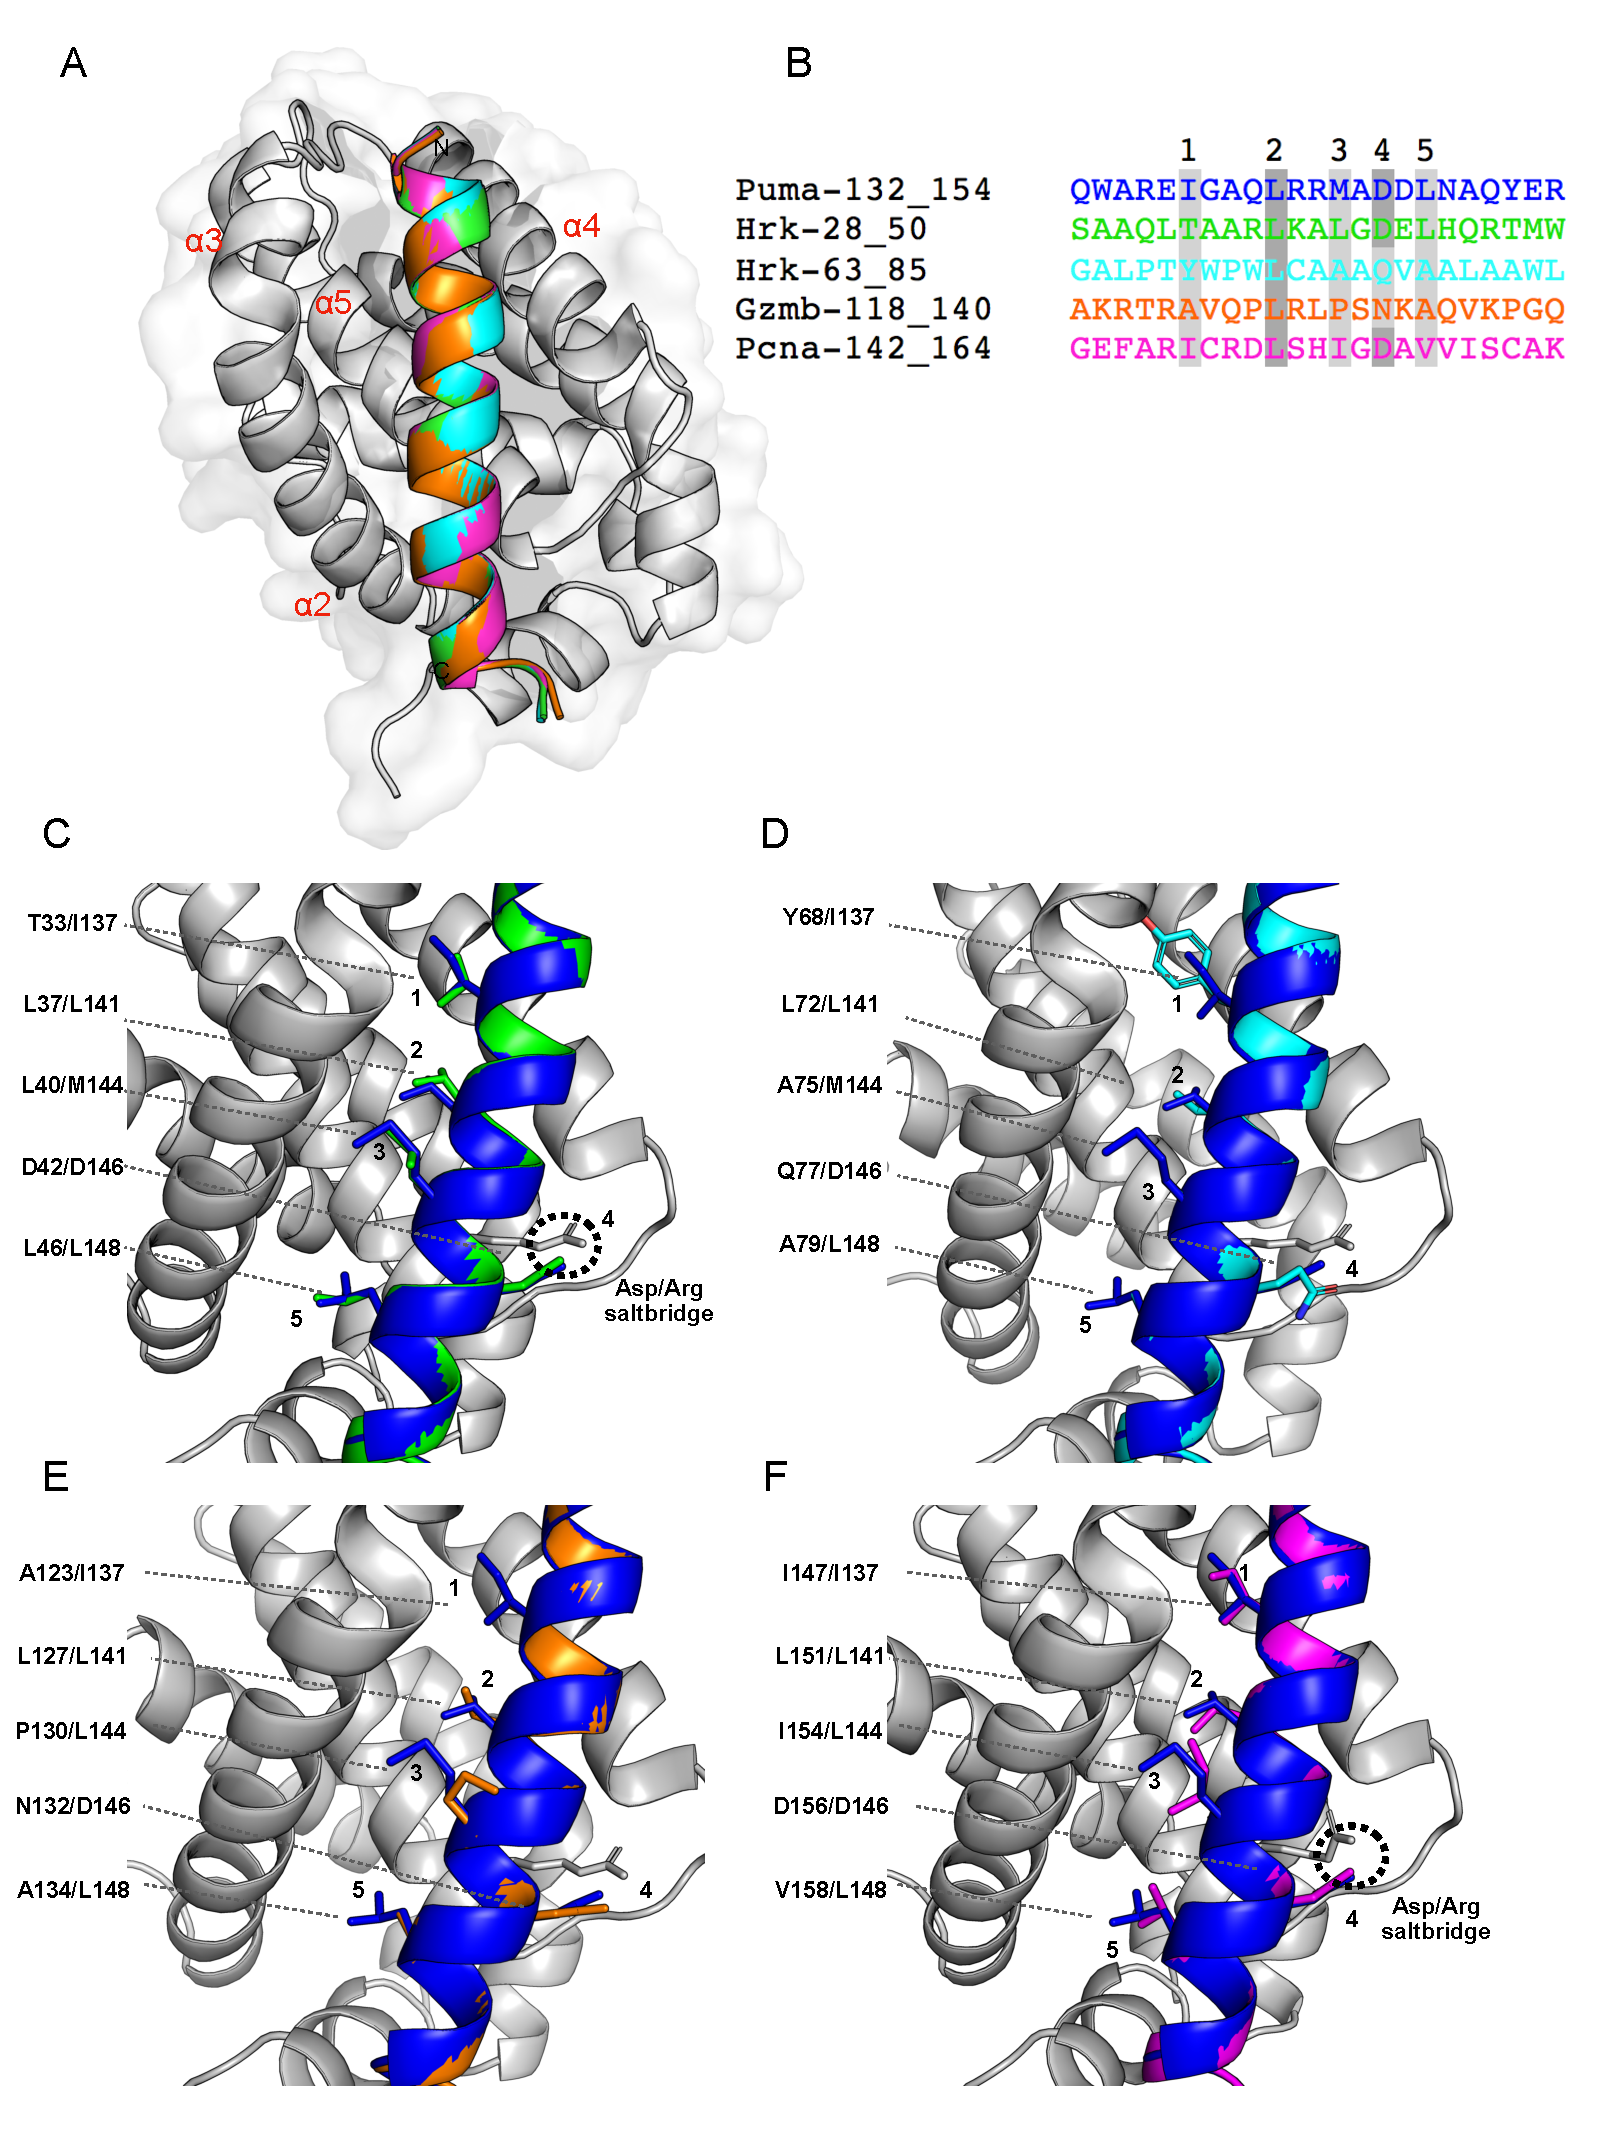
\includegraphics[width=\linewidth]{modelling.pdf}
\caption{{\bf Three-dimensional structure of the modelled complexes.}
A: Superposition of Hrk-28\_50 (Green), Hrk-63\_85 (Cyan), Pcna-142\_164 (Magenta), and Gzmb-118\_140 (Orange) in complex with Bcl2a1 (Grey). B: Multiple-sequence alignments of BH3 motifs. The five residues forming interactions are highlighted in grey with the highly conserved key residues Leu and Asp in darker grey. C,D,E,F: Superposition of the canonical BH3-only peptide Puma-132\_154 (Blue) and the four putative BH3 peptides: C. Hrk-28\_50 (Green), D. Hrk-63\_85 (Cyan), E. Gzmb-118\_140 (Orange), and F. Pcna-142\_164 (Magenta). Sticks and labels show side chain positions of the five residues anchoring the BH3 helix to the hydrophobic surface cleft of the pro-survival proteins. Aspartate residues present in Puma-132\_154, Hrk-28\_50, and Pcna-142\_164 forms a salt bridge with a conserved arginine residue present in the pro-survival proteins.}
\label{fig6}
\end{figure}


\subsubsection*{Superposition of 3D structures}

The superposition of the four putative BH3 peptides and canonical BH3-only peptide Puma (Fig~\ref{fig6} C-F) highlights the resemblance between the five residues in the binding interface, suggesting that these putative BH3 peptides possess the ability to bind pro-survival Bcl2a1.
Fig~\ref{fig6} C shows the BH3 peptide Hrk-28\_50 compared to Puma-132\_154. Our consensus BH3 motif defines the first residue as hydrophobic, matching Leu32 (Fig~\ref{fig6} B). Barrera-vilarmau et al.~\cite{Barrera-Vilarmau2011} resolved a fragment of Hrk (residues 22-53; PDB 2L58) by NMR (Nuclear Magnetic Resonance) and circular dichroism to acquire detailed atomic information on the conformational preference. They identified Thr33 opposed to Leu32 as the key residue in binding Bcl-2 and Bcl-xl. Contemplating these findings, we ultimately modelled the complex Bcl2a1-Hrk-28\_50, aligning Thr33 as the first binding residue. The comparison of Hrk-28\_50 and Puma-132\_154 shows that position 2,3, and 5 are hydrophobic residues. Position 2 and 4 being the conserved leucine and aspartate. Position 1 being the deviant in the comparison with the aforementioned non-hydrophobic Thr33 compared to the hydrophobic Ile137. 

A number of BH3-only proteins have been predicted to contain a transmembrane (TM) region, suggesting an outer mitochondrial membrane (OMM) anchoring function~\cite{Sattler2010}. Barrera-vilarmau et al.~\cite{Barrera-Vilarmau2011} revealed a transmembrane region in Hrk (position 69-91). Given these results, we expect this peptide to be part of the TM region and have a role in membrane targeting activities. 
Fig~\ref{fig6} D shows in accordance to the defined consensus motif and the compared Puma-132\_154, the four hydrophobic residues at position 1, 2, 3, and 5 (small side-chain of Ala74 somewhat hidden). Position 4 comprises a glutamine (Q77) residue opposed to the aspartate in Puma-132\_154 (D146). Despite aspartate being a highly conserved key residue in the BH3 motif, other residues at this position have been reported. For example, pro-autophagic protein AMBRA1 has been demonstrated to act as an inhibitor of pro-survival Bcl-2 by a direct binding through a BH3-like motif containing a glutamine residue instead of the conserved aspartate~\cite{Strappazzon2016}. Another example is found in the BNip group of proteins, a relative new subclass of BH3 proteins. BNip2, seemingly exerting pro-apoptopic effects by inhibiting pro-survival Bcl-2 members, contains a less conserved BH3 motif, in which the conserved aspartate is substituted by a asparagine~\cite{Zhang2003}.
We believe that interactions from other residues at this position, with similar size and chemical properties, are likely to provide sufficient strength, preserving the binding equilibrium. We recognize, that the general understanding of energetic contributions of salt bridges, such as those contributing to the binding between an aspartate in BH3-only proteins and an arginine in glubular Bcl-2 members, is still somewhat unclear. For example, a study by Tomlinson et al.~\cite{Tomlinson2009}, examined salt bridges present in crystal structures of the B1 domain of protein G (GB1). NMR experiments from the study suggested that salt bridges in crystal structures, were not in fact formed in solution. Building on this study, a computational approach was taken by Ahmed et al.~\cite{Ahmed2018}, examining the accuracy of force fields in determining salt bridge strengths in GB1. They found that molecular dynamics simulations, implementing a range of force fields, compared to NMR data, have a tendency to overestimate the stability of salt bridge interactions.

A similar observation of ambiguity in the motif is seen in Gzmb-118\_140 (Fig~\ref{fig6} E), where position 4 is a asparagine (N132) opposed to the aspartate (D146), whereas position 1,2,3, and 5 are hydrophobic residues alike Puma-132\_154.

Out of the four peptides, Pcna-142\_164 (Fig~\ref{fig6} F) presents the most native-like BH3 motif, including the four hydrophobic residues (1,2,3, and 5) as well as the conserved aspartate (4). 

\smallskip

Conclusively, the superposition highlights the analogy between the canonical BH3-only peptide Puma and the four putative BH3 peptides from this study. It is noteworthy that all peptides contains the highly conserved key residue leucine at position (2) and that all peptides contains the hydrophobic residues at position 1,2,3, and 5, with the exception of Thr33 in Hrk-28\_50. Lastly Hrk-28\_50 and Pcna-142\_164 encompasses the conserved key residue aspartate at position 4, whereas Hrk-63\_85 and Gzmb-118\_140 deviate at this position.


%PLOS does not support heading levels beyond the 3rd (no 4th level headings).
\subsection*{Identification of Cancer Mutations and structure-based prediction of functional impact of mutations}

Five missense mutations, originating from breast cancer genomics projects, were identified by exploiting the databases \textit{cBioPortal} and \textit{COSMIC}. Three mutations are reported in Bcl2a1 (M75R (wt-position-mutant), L99R, and V145L), while one mutation is reported in respectively, Gzmb (G50S) and Pcna (Q125H). We used structure-based methods to predict the functional impact upon mutations.

\smallskip

Using the in-house Python wrapper, \textit{MutateX}, developed for high-throughput \textit{in silico} mutagenesis, we carried out a saturation scan of the complete complexes between Bcl2a1 and the putative BH3-like peptides.
\textit{MutateX} relies on the \textit{FoldX} energy function that provides a accurate quantitative estimation of the importance of the intermolecular interactions contributing to the stability of proteins. The energy function allows for the calculation of the change in free energy $(\Delta\Delta G)$ upon mutations, both concerning protein stability and complex formation~\cite{Nygaard2016, Guerois2002}. 
$\Delta\Delta G$ values that does not change upon mutation indicates that the original residue is not essential for protein stability and complexes formation. Negative $\Delta\Delta G$ values indicate that the mutant is more stable than the wild-type (WT), whereas positive $\Delta\Delta G$ indicates that the mutant has a destabilising effect and that the WT may have an important function in preserving the structural integrity of the protein or complex. We considered $\Delta\Delta G$ values larger than 1.6 kcal/mol as deleterious mutations. Mutant variants with $\Delta\Delta G$ \textgreater0 have a decreased protein-protein binding affinity and mutants variant with $\Delta\Delta G$ \textgreater1.6 are likely to have a deleterious effect on the stability and binding affinity~\cite{Nygaard2016}. 

\smallskip

The high-throughput mutational approach allowed us to evaluate the effects of substituting WT residues at the BH3 binding interface of our complexes, with the mutant variants found in cancer patients, but also to evaluate the general effects of any amino-acid substitution. The latter could prove a valuable source of information for future studies, likely identifying new cancer mutation in the proteins under investigation. Additionally, an increased knowledge of hotspot residues for protein-peptide binding between Bcl2a1 and putative BH3-like proteins could potentially aid in the design of selective peptide inhibitors targeting Bcl2a1. 

\subsubsection*{Impact of mutations on binding interface}

The heatmaps in Fig~\ref{fig7} A-C depict the results of the mutagenesis scan of complex Bcl2a1-Hrk-28\_50 (chain A - chain B), while Fig~\ref{fig7} D depicts a color gradient indicating average ($\overline{x}$) $\Delta\Delta G$ in the complex. Overall it is evident that effects of substitution is prevalent in the binding interface. That is, the $\alpha$-helices comprising the hydrophobic surface cleft in Bcl2a1 ($\alpha$2, $\alpha$3, $\alpha$4, and $\alpha$5), as well as the putative BH3 peptide. A substitution in leucine (LA52; residue-chain-position) located in the border line between $\alpha$2 and $\alpha$3 (Fig~\ref{fig7} A), flanking the BH3 peptide, is predicted sensitive to any amino acid substitution ($\overline{x}$ 2.2 kcal/mol), with the exception of a methionine substitution. Methionine shares many properties with aliphatic residues such as leucine, and as such often play a role in binding of hydrophobic ligands. Valine (VA74), with an average $\Delta\Delta G$ of 2.7 kcal/mol is located in $\alpha$4 (Fig~\ref{fig7} B), flanking the BH3 peptide, opposing $\alpha$2 and $\alpha$3. VA74 is predicted to be highly sensitive to substitutions with the polar amino acids arginine, histidine, lysine, and glutamate (to a lesser extent), as well as the aromatic and larger amino acids phenylalanine, tryptophan, and tyrosine. Somewhat surprisingly, a substitution to the mutually aliphatic leucine is predicted to be badly tolerated. Glycine (GA87) and arginine (RA88) are positioned on $\alpha$5 (Fig~\ref{fig7} B), the central hydrophobic helix, constituting the helical bundle interface. A substitution in GA87 is predicted to be extremely affected by any substitution ($\overline{x}$ 20.1 kcal/mol). This effect is likely a result of both the unique properties of glycine, i.e., only containing a hydrogen as its side chain, as well as an \textit{FoldX} overestimation. The small nature of glycine means, that when being in the hydrophobic core, substituting it to a amino acids with a larger side chain, will most likely have severe affect on the stability. This is demonstrated by the somewhat less severe affect (4.4 kcal/mol) of substituting glycine with the second smallest amino acid alanine. Moreover, effects of glycine substitutions are contemplated to be overestimated by \textit{FoldX}, presumably failing to accurately calculate contributions from conformational changes which have not been sufficiently sampled~\cite{Tiberti}. Based on the modelled complexes and the proximity of the centers of charge (\textless 4 \r{A}), we identified the RA88, as the arginine residue putatively forming salt bridge interactions with the conserved aspartate found in Hrk-28\_50 and Pcna-142\_164. The positively charged arginine (RA88) forms interactions with the negatively charged conserved aspartate. As a result, RA88 is highly sensitive to substitutions to the negatively charged acidic amino acids aspartate and glutamate. The involvement of RA88 is highlighted by the predicted sensitivity ($\overline{x}$ 2.0 kcal/mol) to most substitutions, even the likewise positively charged lysine. The most tolerated substitution is to a histidine, something that could be explained by its unique chemical properties. The side chain of histidine has a $pK_{a}$ close to physiological pH, implicating that a local environment determined shifts in pH, will change its average charge. Consequently, a population of protonated positively charged histidines can be expected at physiological conditions~\cite{Betts2007}. Therefore it can be suggested that the toleration of this substitution is due to the alike capability of forming electrostatic salt bridge interactions. 

\smallskip

Fig~\ref{fig7} C depicts substitutions affecting the putative BH3 peptide and the important binding residues. TB33, the position earlier identified as one of the residues contributing to the binding in the BH3 motif, is intriguingly predicted to increase binding energies ($\Delta\Delta G$ \textless0) when substituted to a hydrophobic amino acid in the form of either: one of the aliphatic amino acids, alanine, valine, leucine, and methionine (aliphatic-like) or the aromatic phenylalanine. Thus, suggesting that a hydrophobic residue at this position, as most often observed in canonical BH3 motifs, is more favorable in terms of binding affinity. Position AB34 is predicted highly intolerant ($\overline{x}$ 7.8 kcal/mol) to any substitution except for a glycine, which increases the stability. As aforementioned, this is most likely a result of size, with a substitution to the smaller glycine as the only tolerated substitution. Substitution in the canonical BH3 motif conserved key leucine LB37 is predicted sensitive to most substitutions ($\overline{x}$ 2.1 kcal/mol). LB37 moderately tolerates substitutions by the hydrophobic amino acids valine, isoleucine, and methionine as well the somewhat amphipathic lysine. The substitution of the basic lysine (KB38) with any amino acids except arginine, valine, leucine, and methionine, decreases the binding affinity($\overline{x}$ 1.8 kcal/mol). Hence, suggesting a role in the binding site feasibly through electrostatic interactions, indicated by the increased affinity induced by substitution to the other positively charged amino acid, arginine. Regarding the low sensitivity to substitutions to valine, leucine, and methionine, this can be thought of as a result of the placement in the hydrophobic core, favoring hydrophobic residues.
The hydrophobic leucines LB40 and LB44, contributing to the complex formation, are predicted to tolerate substitution by most aliphatic and aromatic amino acids. Substitution in GB41 results in the same effect as discussed earlier when substituting the small glycine buried in the hydrophobic core. Substitution in the BH3 motif conserved and putatively salt-bridge forming aspartate (DB42) is mostly predicted intolerable ($\overline{x}$ 1.8 kcal/mol). DB42 can be substituted without any noteworthy effects, to the polar amino acids: (i) glutamate, which is similarly negatively charged, (ii) asparagine, which differs only in, that it contains an amino group, and (iii) glutamine.  

\clearpage
\begin{figure}[hp!]
% \includegraphics[width=\linewidth]{mutagenesis_Hrk.pdf}
\includegraphics[width=1.4\textwidth,right]{mutagenesis_Hrk.pdf}%
\caption{{\bf Effects of substitutions on protein-peptide complexes upon \textit{in silico} saturation mutagenesis scan of Bcl2a1-Hrk-28\_50.}
A,B,C: Heatmaps based on calculations of $\Delta\Delta G$ for substitutions affecting the binding interface. Horizontal labels show wild-type (WT) amino acids (residue-chain-position). Vertical labels show the variant amino acids, including all 20 natural occurring amino acids. Color bar indicates the range of $\Delta\Delta G$ values (kcal/mol). A: Bcl2a1 $\alpha$-helix 2 (32-52) and 3 (53-58). B: Bcl2a1 $\alpha$-helix 4 (66-80) and 5 (86-105). C: Hrk putative BH3 $\alpha$-helix (28-50). D: Color gradient indicating average $\Delta\Delta G$ (Bcl2a1, white to red and Hrk-28\_50, yellow to orange). The residues estimated to be most important ($\Delta\Delta G$\textgreater1.6) for binding affinity are labeled. Spheres indicate position of reported cancer mutations M75R, L99R, and V145L (labeled in blue).} 
\label{fig7}
\end{figure}

Conclusively, the mutagenesis scan of Bcl2a1-Hrk-28\_50 pointed to a subset of substitutions with damaging effects on the complex formations. These results suggest the importance of: (i) hydrophobic residues in binding the amphiphatic helix comprising the BH3 motif, (ii) the disadvantageous in terms of binding affinity of threonine (TB33) compared to a hydrophobic amino acid, (iii) the electrostatic interactions between arginine (RA88) and the conserved aspartate (DB42), and (iv) the conserved leucine (LB37) in terms of its low susceptibility to substitutions

\smallskip

The three reported cancer mutations in Bcl2a1, M75R, L99R, and V145L are not located in sites (Fig~\ref{fig7} D) predicted to affect the Bcl2a1-Hrk-28\_50 complex formation. The $\Delta\Delta G$ of the mutant variants M75R, L99R, and V145L are respectively -0.17, -0.06, and -0.008 and therefore, in fact predicted to increase binding affinity compared to the WT. 

\smallskip

The \textit{FoldX} energy function is limited by its capability of only predicting local effects of substitutions and as such will disregard allosteric effects of mutations located at distal site, with respect to the binding interface~\cite{Nygaard2016}. The three cancer mutations are not predicted to interact directly in the biding but might have allosteric effects on the residues involved in the binding. Consequently, possible indirect effects of three mutations might not be captured by the mutagenesis scan.


\subsubsection*{Impact of mutations on the structural stability}

In addition to predicting the effect of cancer mutation on the complex formation, we carried out a saturation scan on the free-state Bcl2a1 protein. This allowed us to predict the impacts of the three cancer mutation on the protein structural stability. We note, that no experimentally derived free-state Bcl2a1 structure exists. As a result, we conducted the scan on a manipulated (dismissed Puma peptide) Bcl2a1-Puma complex and as such, the effect of the binding interface, induce some uncertainties on the general stability of the free-state. 
Fig~\ref{fig8} A depicts the top 20 most affected residues in Bc2a1 in terms of average $\Delta\Delta G$ upon substitutions. A pattern can be seen of residues being predicted highly destabilizing: (i) small amino acids ($\overline{x}$ 8-13 kcal/mol): glycine, alanine, and serine and (ii) hydrophobic amino acids such as the aliphatic: alanine, methionine, valine, leucine, and isoleucine, as well as the aromatic: phenylalanine and tryptophan ($\overline{x}$ 5-8 kcal). The large impact of substituting small residues is, as aforementioned, likely an effect of both the nature of substituting smaller to larger, as well as an overestimation of \textit{FoldX}. The large impact of substituting the hydrophobic residues is likely a result of their involvement in binding and preferred location in the protein interior~\cite{Betts2007}. The missense mutation M75R is depicted as one of the 20 most destabilizing substitutions with an average $\Delta\Delta G$ of 5.3kcal/mol. 

Fig~\ref{fig8} B shows the results of the mutagenesis scan of Bcl2a1, depicting the effects of substitutions in the three sites mapped by the cancer mutations. Substituting position MA75 to the mutant variant arginine, is predicted to have a destabilizing effect (3.3 kcal/mol) on the protein stability. Similarly, substituting the position LA99 to the mutant variant, arginine, is predicted to have a destabilizing effect (6.3 kcal/mol). While substituting the position VA145 to the mutant variant leucine is not predicted to have an effect (0.14 kcal/mol) on the stability. Collectively for the two destabilizing mutations, it is substitution of hydrophobic residues, buried in the interior of the protein (Fig~\ref{fig7} D) to the polar arginine, which regardless of it amphiphatic nature, exerts a destabilizing effect. On the other hand, substituting the mutually aliphatic amino acids V145L does not impact on the stability of Bcl2a1. 
\clearpage
\begin{figure}[hp!]
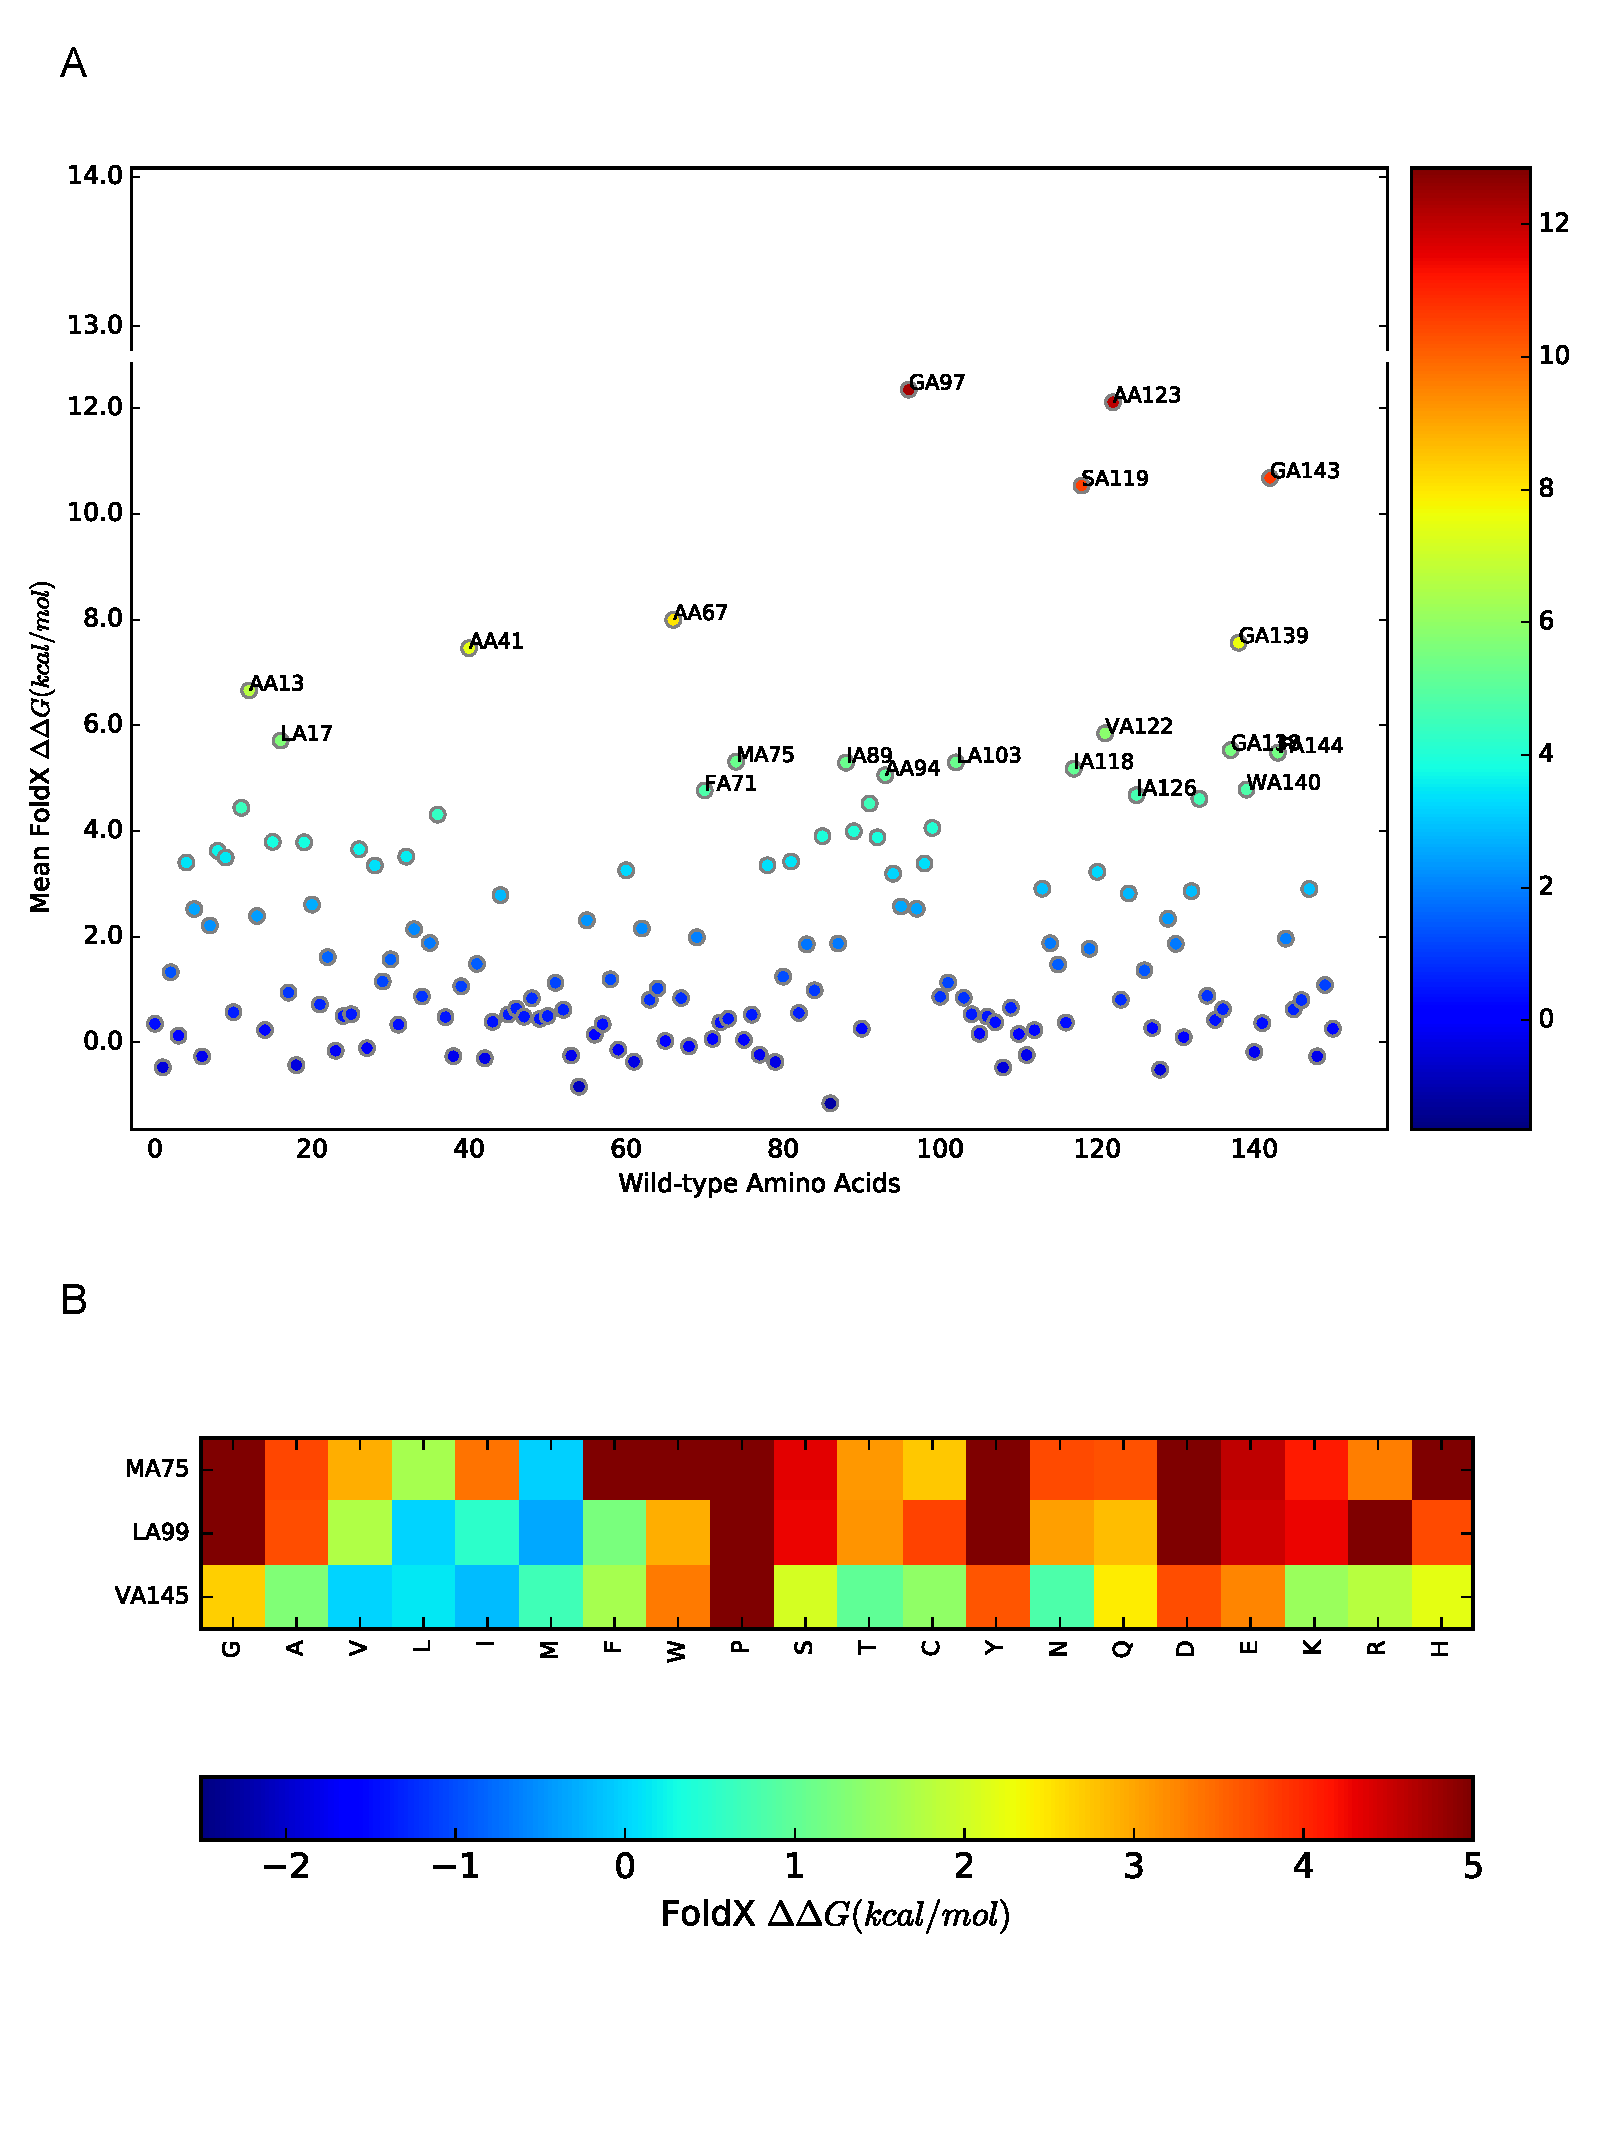
\includegraphics[width=\linewidth]{free_state.pdf}
\caption{{\bf Effects of substitutions on free-state protein stability upon \textit{in silico} saturation mutagenesis scan of Bcl2a1.}
A: Scatter plot depicting the mean $\Delta\Delta G$ for substitution of wild-type (WT) amino acids. The x-axis shows the spread of WT amino acids. The top 20 most destabilizing positions are labeled. Labels follows the convention: residue type, chain, and residue number. B: Heatmap based on calculations of $\Delta\Delta G$ for substitutions in the three WT amino acids MA75, LA99, and VA145. Vertical labels show wild-type (WT) amino acids (residue-chain-position). Horizontal labels show the variant amino acids, including all 20 natural occurring amino acids. Color bar indicates the range of $\Delta\Delta G$ values (kcal/mol).} 
\label{fig8}
\end{figure}


With the aim of this study in mind (i.e., being a presentation of a workflow), we concluded not to include the saturation scans of the three complexes Hrk-63\_85, Pcna-142\_164, and Gzmb-118\_140. We feel that the above presentation suffice to deliver a clear idea about the usefulness of an \textit{in silico} mutagenesis approach to structure-based prediction of impact of substitutions.

To the interested, the modelled complexes Hrk-63\_85, Pcna-142\_164 and Gzmb-118\_140 and guidelines on how to carry out the \textit{MutateX} scans, can be found at our GitHub repository (https://github.com/ELELAB/bcl2\_bh3\_breast\_cancer).

\section*{Discussion}
The network of protein–protein interactions between globular Bcl-2 family members and their BH3-only interactors plays an important role in controlling tissue homeostasis and deregulation can lead to cancer development. An increased understanding of both the transciptomic signatures, as well as the molecular mechanism of pro-survival Bcl-2 members, will likely guide advantages in therapeutically targeting these proteins. Through this study, we present a workflow aimed at providing insight into: (i) the expression of pro-suvival Bcl-2 members and their interactors, as well as (ii) elucidating the functional interaction between them, and predicting effects of substitutions on the interaction. We applied this workflow on the BRCA data from \textit{The Cancer Genome Atlas (TCGA)}~\cite{Chang2013}, but it is just as applicable to other cancer dataset on \textit{TCGA}.

Despite the importance of the Bcl-2 family conserved BH3 motif in mediating protein–protein interactions, a validated BH3 consensus motif is elusive~\cite{Aouacheria2013}. We defined our take on the motif, contemplating previously described motifs~\cite{Day2008, Hawley2012}, alignments of canonical BH3 motifs, and knowledge of conserved residues~\cite{Sattler2010}. We allowed for flexibility in some of the conserved positions, as to prevent the discrimination of possible BH3-like proteins. The motif was applied to filter interaction partner of the Bcl-2 family members, extracted from the \textit{Integrated Interactions Database}~\cite{Kotlyar2016}.


Pro-survival members are shown to be upregulated in a variety of tumor types~\cite{Rochaix1999, Strik1999, 10.2307/1693640, Placzek2010} and have additionally been considered to contribute to tumorigenesis and therapeutic resistance~\cite{Bae2006, Adams2007, Kim2012}. It is thus apparent, that studies into the expression of the pro-survival members at the mRNA level is necessary to guide and optimize the anti-cancer treatments.
From the analysis of the \textit{TCGA} BRCA dataset, we uncovered the gene expression landscape of globular Bcl-2 members and their putative BH3-like interactors.
We found the pro-survival Bcl2a1 gene to be upregulated in tumor tissue. The expression and function of pro-survival Bcl2a1 in normal tissues appears to be linked to the immune system in which, it seems that development of inflammasomes increases the expression of Bcl2a1, consequently protecting pro-inflammatory cells from apoptosis~\cite{Karsan1996, Noble1999}. Moreover, a physiological function of Bcl2a1 in the mammary glands have been identified, in which overexpression of Bcl2a1 in mice has been linked to the prevention of mammary gland involution by apoptosis~\cite{Capuco2002}. 
Regarding the expression in cancer, it is not surprising, when considering its link to the immune system, that Bcl2a1 has been found overexpressed in a variety of hematological malignancies~\cite{Nagy2003}. Besides liquid cancers, Bcl2a1 has been demonstrated to be overexpressed in a variety of solid cancers. Intriguingly, a study comparing a range of solid tumor tissues found the highest expression of Bcl2a1 in breast cancers~\cite{Beverly2009}, while another study comparing expression levels between stages of breast cancer found a association between advanced decease stages and higher expression levels~\cite{Yoon2003}. The association with decease stage suggests that Bcl2a1 may contribute to tumorigenesis.
Apart from the likely role in tumorigenesis, Bcl2a1 induces chemotherapeutic resistance by suppressing apoptosis upon toxic stimulation, consequently preventing cell death. Overexpression of Bcl2a1 in cell lines has been found to promote resistance to a assortment of cancer drugs including the BH3 mimetic ABT-737, a specific inhibitor targeting Bcl-2, Bcl-xl, and Bcl-w~\cite{Yecies2010}.
Due to their significant role as inhibitors of apoptosis, pro-survival Bcl-2 proteins are considered promising targets for anti-cancer therapy. Progress has been made and several BH3 mimetics targeting the hydrophobic cleft in pro-survival members, show promising perspectives. What is common for these mimetics is, that they have either been successful in inhibiting Bcl-2, Bcl-xl, and Bcl-w, but not Mcl1 or Bcl2a1, or they have been broad-spectrum inhibitors with differing affinities. In spite of the general progress, no potent and selective BH3 mimetics, targeting Bcl2a1 has so far been demonstrated~\cite{Vogler2012, Garner2017}. 
Unraveling to what extent putative BH3-like interactors are deregulated in BRCA and additionally clarifying their possible interaction with Bcl2a1 at the structural level, might prove a valuable source of information. Identifying possible Bcl2a1 selective interactors could serve as templates for the design of BH3 mimetics, targeting and preventing its pro-survival role in tumors.

We identified two putative BH3-containing interactors that were deregulated at the mRNA level as well one putative BH3 interactor (Gzmb) that were significantly co-expressed with Bcl2a1. Hrk, encoding Activator of apoptosis harakiri, was found to be downregulated, while Pcna, encoding Proliferating cell nuclear antigen, was found to be upregulated.
We subsequently zoomed in at the structural level of these putative interactors, with the scope of clarifying to what extent they could be thought of as actual BH3-only proteins or mere false-positives, resulting from the complexity of defining the BH3 motif. To do so, we modelled the complexes of Bcl2a1 and the putative interactors, focusing on the canonical key residues in binding of the BH3 motif (peptide) to the hydrophobic cleft found in globular Bcl-2 family members.
A superposition between the template and target structure, highlighted the resemblance between the canonical BH3-only peptide Puma and the four putative BH3 peptides, both in terms of residue positioning on the amphipatic helix and direction towards the binding cleft. Generally, we observed many of the structural characteristics of the canonical BH3 motif. The four peptides all comprises the highly conserved key residue leucine as well as the hydrophobic residues known to provide additional binding interactions (Thr33 exception in Hrk-28\_50). Moreover, they either contains the conserved key residue aspartate (known to form salt bridges) or the residues asparagine/glutamine with somewhat similar chemical properties. Deviations at this key positions has previously been demonstrated in canonical BH3 motifs\cite{Zhang2003,Strappazzon2016}.

Hrk has indeed been reported as a BH3-only protein capable of sensitizing pro-survival proteins, with a higher selectivity towards Bcl-xl, Bcl-w, and Bcl2a1~\cite{Chen2005}. Being a sensitizer, and as such a pro-apoptotic protein, it is not surprising that we found Hrk to be downregulated in cancer. We initially identified two possible BH3 motifs in Hrk. One motif (Hrk-28\_50), corresponding to the canonical cytosolic BH3 motif. The other motif (Hrk-63\_85) is presumable situated in the transmembranic region of Hrk~\cite{Barrera-Vilarmau2011}, thus obstructed to interact with the hydrophobic cleft and as such speculated to be a false-positive match.

Pcna is a cell cycle regulator, that acts as a processivity factor for DNA polymerase $\delta$. It is is involved in, and essential for DNA replication, repair and cell-cycle progression. It has been reported, that Mcl1 binds Pcna by an interaction mediated by a consensus binding motif that is thought to include the BH3 motif. Supporting this, mutations near the BH3-binding cleft disrupt the interaction~\cite{DeBartolo2014}. In this regard, Mcl1 is now thought of having a dual-functional role in cancer, meaning that it possesses the capabilities to acts as both a pro-survival oncogene but also as a anti-proliferative agent by the inhibition of Pcna and cell cycle progression. Pcna is not known to bind to Bcl2a1, but Bcl2a1 and Mcl1 are often grouped together (in the Bcl-2 family) in terms of their binding profile and selectivity to BH3-only proteins~\cite{Vogler2012}. As such, it can be speculated that Bcl2a1 might have the ability to bind Pcna, though we do not find it likely based on available literature. For example, Bartolo et al.~\cite{DeBartolo2014} tested interactions between the pro-survival Bcl-2 members and 36 putative and canonical BH3 peptide using peptide SPOT arrays, and they only found Pcna to interact with Mcl1. We found Pcna to be overexpressed in tumor tissue, something that has been linked to the progression of tumorigenesis and significantly associated with poor survival, and advanced disease stages~\cite{Qiongying2016}.

Gzmb (Granzyme B) is a serine protease, that among many roles, have the capacity to induce apoptosis by either cleaving the pro-apoptotic protein Bid, or by directly activating caspases, permeabilizing the OMM. Moreover, Gzmb can cleave Mcl1, impairing its pro-survival capacity to prevent apoptosis. Gzmb induced apoptosis can be blocked by pro-survival Bcl-2 members, binding and inhibiting its ability to interact and cleave Bid~\cite{Thomas2010, Sutton2012}. 
In spite of the interactions between Gzmb and pro-survival members, we did not find any evidence in the literature of the existence of a BH3 motif in Gzmb. Having shown that the Gzmb-118\_140 peptide possess the characteristics of a canonical BH3 motif, we propose the possibility of Gzmb being a BH3-like protein. At the same time, we acknowledge the need for further experimental elucidation to prove or disprove these \textit{in silico} findings.

We recognize the complications of implicitly assuming that elevated or reduced mRNA levels correspond to a similar pattern in protein expression. The Bcl-2 proteins are influenced by many post-translational modifications, specially phosphorylation and ubiquitylation, that can influence the protein half-life and turnover, consequently effecting the mRNA–protein correlation~\cite{Czabotar2014}.
Several studies have reported a relatively poor agreement in genome-wide correlation between expression levels, of mRNA and proteins, lingering around 50\% explanatory power~\cite{Maier2009}. However, when examining the relationship between differentially expressed mRNA and their protein product, a significantly higher correlation is found~\cite{Koussounadis2015}. As such, this increases our confidence in using differentially expressed mRNA as a measure of protein expression. Nevertheless, we urge people to consider this challenge and if possible, experimentally determine whether the observed changes in mRNA correspond to observed levels in their protein product. 

The quantitative evaluation of the impacts of mutations on both the stability as well as the binding affinity to BH3 interactors, is critical to understand the functional capacity of pro-survival proteins to propagate apoptosis. Drug resistance in anti-cancer treatments continues to be one of the leading reasons for unsuccessful treatments and several studies has linked mutations in Bcl-2 members to altered sensitivity or resistance to BH3-mimetics~\cite{Letai2002,Fresquet2014,Singh2016}. In general, the functional assessment of mutation data have lagged behind the growth of data generated from modern high-throughput techniques. Here, we applied an in-house high-throughput mutagenesis approach, allowing us to computationally predict the effects of mutations found in cancer patients, on both the free-state stability of Bcl2a1, and the binding energies between Bcl2a1 and the three putative BH3 interactors. Moreover, this high-throughput approach permitted us to evaluate the general effects of any amino-acid substitution. Thus, the full saturation scan provides valuable information into functionally important residues and critical hotspots for protein-protein binding.
To address the use of this approach, we carried out a saturation scan of the modelled complex between Bcl2a1 and the cytosolic Hrk-28\_50 peptide. The scan pointed to a subset of substitutions with damaging effects on the binding energies, suggesting the importance of: (i) hydrophobic residues in Bcl2a1, binding the amphiphatic helix comprising the BH3 motif, (ii) the disadvantageous, in terms of binding affinity of thr33 compared to a hydrophobic amino acid, (iii) the electrostatic interactions (saltbridge) between a arginine in Bcl2a1 and the conserved aspartate in Hrk, and (iv) the conserved key residue leucine in terms of its low susceptibility to substitutions. These functionally important residues, in terms of binding concurs with the generally accepted key residues in canonical BH3 motifs~\cite{Hinds2005, Czabotar2007, Sattler2010}. Additionally the scan pointed to a decreased binding affinity, when substituting a lysine (KB38) found in the middle of the BH3 motif. Possible, suggesting a previously undescribed role in the binding site.

Lastly, we zoomed in on the three mutations in Bcl2a1, found in cancer patients in the databases \textit{cBioPortal}~\cite{Cerami2012} and \textit{COSMIC}~\cite{Forbes2017}. First, we recognize that a limited number of mutation have been reported in pro-survival proteins, as destabilizing mutations would likely cause an increased rate of apoptosis, which is more frequently impaired in cancer.
The mutations were not predicted to effect the binding affinity and formation of the Bcl2a1-Hrk-28\_50 complex. However, when evaluating the effect of the mutations on the protein structural stability of the free-state Bcl2a1 protein, we found two of the mutant variant, predicted highly destabilizing and thus, likely detrimental on the integrity of the protein structure.

Finally, we would like to address the future directions of this study. We would like to incorporate transcriptomic profiling data of normal tissue sites from \textit{The Genotype-Tissue Expression (GTEx)} portal (https://www.gtexportal.org/home/) into our analysis. Transcriptomic data from \textit{TCGA} only include around 10\% normal samples and additionally these samples are collected adjacent (\textgreater2 cm) to tumor samples. Combining the data from \textit{GTEx} and \textit{TCGA} would allow for a better characterization between the treatments (tumor/normal) and a more balanced dataset. Regarding the DEA, we will include PAM50 molecular subtype information to clarify the expression patterns, not only between tumor and normal but also between molecular subtype's. This would hopefully provide a more "clear" picture of the gene expression landscape of pro-survival members in a heterogeneous disease, such as breast cancer. Moreover, it would be intriguing to include additionally possible sources of variation into our exploratory analysis, with the aim of identifying additional variables that could help explaining the spread in the data. For example, it would be interesting to include clinical information, such as possible drug treatments of patients, as this could conflict with our interpretation of DE (e.g., treatments targeting pro-survival members).
We would also like to take a more robust and refined approach to the analysis of co-expression, by implementing the \textit{R} package \textit{WGCNA}, computing weighted gene co-expression network analysis, that can be used to identify modules of highly correlated genes. Concerning the complications of the relationship between mRNA and protein levels, we would like to compare the expression of mRNA levels of candidate genes observed in this study to proteomics data from \text{The CPTAC Data Portal} (https://proteomics.cancer.gov/data-portal), acquired for 105 \textit{TCGA} BRCA samples. Regarding the structural elucidation of the complex formation between Bcl2a1 and the putative BH3-like interactors, we would like to apply molecular dynamics simulations. This could allow further assessment of the reliability of the interactions in the complexes.   

\section*{Conclusion}
We have proposed a ‘multiscale’ approach to unravel the pro-survival Bcl-2 signature in cancer, bridging global changes such as changes in the expression levels and mutations of the pro-survival Bcl-2 members and their putative BH3-like interactors. We have provided a computational workflow to uncover the gene expression landscape and to analyze the structural and functional effects of mutations on the binding affinity and structural stability. Moreover, we have proposed a high-throughput \textit{in silico} mutagenesis approach to identify functionally important residues in the pro-survival members and their interactors. Our study highlights the prospects of an integrative bioinformatic approach, as it could potentially aid the development of selective inhibitors, by identifying substitutions in pro-survival BH3-only interactors that would reduce binding to other pro-survival members without substantially weakening the binding to the target.
Lastly, we note that the approach to pro-survival proteins, proposed here, can just as well be applied to pro-apoptotic members. For example, the evaluation of cancer mutation in terms of classifying them as driver mutation or passenger mutation, would be highly relevant with a focus on pro-apoptotic members. 


\section*{Supporting information}

% Include only the SI item label in the paragraph heading. Use the \nameref{label} command to cite SI items in the text.
\paragraph*{S1 Fig.}
\label{S1_Fig}
{\bf Protein-protein network.}
Network of pro-survival Bcl-2 proteins (Label color, red) and their known interactors containing the BH3 motif. The node size is determined by the degree of interactions).

\paragraph*{S2 Fig.}
\label{S2_Fig}
{\bf Heatmap of log-CPM values for the 45 differentially expressed candidate genes.}
The values are clustered by columns (samples) and rows (genes), with dendrogram indicating how clusters are formed. The color-scale represent gene expression magnitude (High expression, red; Low expression, Blue).

\section*{Acknowledgments}
I would like to thank my colleges at the Computational Biology Laboratory (DCRC) for allowing me to be a part of their group, while working on my masters project, as well as providing useful discussions. A special thanks to my supervisors, Matteo Lambrughi, Thilde Bagger Terkelsen, and professor Elena Papaleo for their guidance and support. I would also like to appreciate my gratitude to Björn Canbäck, coordinator for the Master programme in Bioinformatics, for his support during my studies, without which, I might not have come to the point of handing in a degree projects in Bioinformatics.

This project is supported by a grant from the LEO Foundation (number LF17006) to EP group.

\nolinenumbers

% Use the PLoS provided BiBTeX style
\bibliographystyle{plos2015}

% uncomment and compile bibtex to update bbl file. Paste bbl content to the paper and compile to laxex (twice).
% \bibliography{library} 

% Compile your BiBTeX database using our plos2015.bst
% style file and paste the contents of your .bbl file
% here. See http://journals.plos.org/plosone/s/latex for 
% step-by-step instructions.
\begin{thebibliography}{100}

\bibitem{Reed1999}
Reed JC.
\newblock {Dysregulation of apoptosis in cancer}.
\newblock Journal of Clinical Oncology. 1999;17(9):2941--2953.
\newblock doi:{10.1200/JCO.1999.17.9.2941}.

\bibitem{Kroemer2009}
Kroemer G, Galluzzi L, Vandenabeele P, Abrams J, Alnemri ES, Baehrecke EH,
  et~al.
\newblock {Classification of cell death: Recommendations of the Nomenclature
  Committee on Cell Death 2009}.
\newblock Cell Death and Differentiation. 2009;16(1):3--11.
\newblock doi:{10.1038/cdd.2008.150}.

\bibitem{Villunger2003}
Villunger A, Michalak EM, Coultas L, M{\"{u}}llauer F, B{\"{o}}ck G,
  Ausserlechner MJ, et~al.
\newblock {p53- and Drug-Induced Apoptotic Responses Mediated by BH3-Only
  Proteins Puma and Noxa}.
\newblock Science. 2003;302(5647):1036--1038.
\newblock doi:{10.1126/science.1090072}.

\bibitem{Strasser2009}
Strasser A, Jost PJ, Nagata S.
\newblock {The Many Roles of FAS Receptor Signaling in the Immune System}.
\newblock Immunity. 2009;30(2):180--192.
\newblock doi:{10.1016/j.immuni.2009.01.001}.

\bibitem{Kerr1972}
Kerr JF, Currie AR, Wyllie AH.
\newblock {Apoptosis: a Basic Biological Phenomenon With Wide- Ranging
  Implications in Tissue Kinetics}.
\newblock Journal of Internal Medicine. 1972;258(6):479--517.
\newblock doi:{10.1111/j.1365-2796.2005.01570.x}.

\bibitem{Nagata2010}
Nagata S, Hanayama R, Kawane K.
\newblock {Autoimmunity and the Clearance of Dead Cells}.
\newblock Cell. 2010;140(5):619--630.
\newblock doi:{10.1016/j.cell.2010.02.014}.

\bibitem{Edlich2017}
Edlich F.
\newblock {BCL-2 proteins and apoptosis: Recent insights and unknowns}.
\newblock Biochemical and Biophysical Research Communications.
  2017;doi:{10.1016/j.bbrc.2017.06.190}.

\bibitem{Heimlich2004}
Heimlich G, McKinnon AD, Bernardo K, Brdiczka D, Reed JC, Kain R, et~al.
\newblock {Bax-induced cytochrome c release from mitochondria depends on
  alpha-helices-5 and -6}.
\newblock Biochemical Journal. 2004;378(1):247--255.
\newblock doi:{10.1042/bj20031152}.

\bibitem{Zheng2016}
Zheng JH, {Viacava Follis} A, Kriwacki RW, Moldoveanu T.
\newblock {Discoveries and controversies in BCL-2 protein-mediated apoptosis}.
\newblock FEBS Journal. 2016;283:2690--2700.
\newblock doi:{10.1111/febs.13527}.

\bibitem{Czabotar2014}
Czabotar PE, Lessene G, Strasser A, Adams JM.
\newblock {Control of apoptosis by the BCL-2 protein family: Implications for
  physiology and therapy}.
\newblock Nature Reviews Molecular Cell Biology. 2014;15(1):49--63.
\newblock doi:{10.1038/nrm3722}.

\bibitem{Um2015}
Um HD.
\newblock {Bcl-2 family proteins as regulators of cancer cell invasion and
  metastasis : a review focusing on mitochondrial respiration and reactive
  oxygen species}.
\newblock Oncotarget. 2015;7(5):5193--5203.
\newblock doi:{10.18632/oncotarget.6405}.

\bibitem{Kvansakul2008}
Kvansakul M, Yang H, Fairlie WD, Czabotar PE, Fischer SF, Perugini MA, et~al.
\newblock {Vaccinia virus anti-apoptotic F1L is a novel Bcl-2-like
  domain-swapped dimer that binds a highly selective subset of BH3-containing
  death ligands}.
\newblock Cell Death and Differentiation. 2008;15(10):1564--1571.
\newblock doi:{10.1038/cdd.2008.83}.

\bibitem{Muchmore1996}
Muchmore SW, Sattler M, Liang H, Meadows RP, Harlan JE, Yoon HS, et~al.
\newblock {X-ray and NMR structure of human Bcl-xL, an inhibitor of programmed
  cell death}.
\newblock Nature. 1996;381(6580):335--341.
\newblock doi:{10.1038/381335a0}.

\bibitem{Hardwick2013}
Hardwick JM, Soane L.
\newblock {Multiple functions of BCL-2 family proteins}.
\newblock Cold Spring Harb Perspect Biol. 2013;5(2).
\newblock doi:{10.1101/cshperspect.a008722 a008722 [pii] 5/2/a008722 [pii]}.

\bibitem{Hinds2007}
Hinds MG, Smits C, Fredericks-Short R, Risk JM, Bailey M, Huang DCS, et~al.
\newblock {Bim, Bad and Bmf: Intrinsically unstructured BH3-only proteins that
  undergo a localized conformational change upon binding to prosurvival Bcl-2
  targets}.
\newblock Cell Death and Differentiation. 2007;14(1):128--136.
\newblock doi:{10.1038/sj.cdd.4401934}.

\bibitem{Letai2002}
Letai A, Bassik MC, Walensky LD, Sorcinelli MD, Weiler S, Korsmeyer SJ.
\newblock {Distinct BH3 domains either sensitize or activate mitochondrial
  apoptosis, serving as prototype cancer therapeutics}.
\newblock Cancer Cell. 2002;2(3):183--192.
\newblock doi:{10.1016/S1535-6108(02)00127-7}.

\bibitem{Kuwana2005}
Kuwana T, Bouchier-Hayes L, Chipuk JE, Bonzon C, Sullivan BA, Green DR, et~al.
\newblock {BH3 domains of BH3-only proteins differentially regulate
  Bax-mediated mitochondrial membrane permeabilization both directly and
  indirectly}.
\newblock Molecular Cell. 2005;17(4):525--535.
\newblock doi:{10.1016/j.molcel.2005.02.003}.

\bibitem{Shamas-din2016}
Shamas-din A, Kale J, Leber B, Andrews DW.
\newblock {Mechanisms of Action of Bcl-2 Family Proteins}.
\newblock Cold Spring Harb Perspect Biol. 2016; p. 1--22.

\bibitem{Llambi2011}
Llambi F, Moldoveanu T, Tait SWG, Bouchier-Hayes L, Temirov J, McCormick LL,
  et~al.
\newblock {A Unified Model of Mammalian BCL-2 Protein Family Interactions at
  the Mitochondria}.
\newblock Molecular Cell. 2011;44(4):517--531.
\newblock doi:{10.1016/j.molcel.2011.10.001}.

\bibitem{Aouacheria2013}
Aouacheria A, {Rech de Laval} V, Combet C, Hardwick JM.
\newblock {Evolution of Bcl-2 homology motifs: Homology versus homoplasy}.
\newblock Trends in Cell Biology. 2013;23(3):103--111.
\newblock doi:{10.1016/j.tcb.2012.10.010}.

\bibitem{DeBartolo2014}
DeBartolo J, Taipale M, Keating AE.
\newblock {Genome-Wide Prediction and Validation of Peptides That Bind Human
  Prosurvival Bcl-2 Proteins}.
\newblock PLoS Computational Biology. 2014;10(6).
\newblock doi:{10.1371/journal.pcbi.1003693}.

\bibitem{Aouacheria2015}
Aouacheria A, Combet C, Tompa P, Hardwick JM.
\newblock {Redefining the BH3 Death Domain as a 'Short Linear Motif'}.
\newblock Trends in Biochemical Sciences. 2015;40(12):736--748.
\newblock doi:{10.1016/j.tibs.2015.09.007}.

\bibitem{Chen2005}
Chen L, Willis SN, Wei A, Smith BJ, Fletcher JI, Hinds MG, et~al.
\newblock {Differential targeting of prosurvival Bcl-2 proteins by their
  BH3-only ligands allows complementary apoptotic function}.
\newblock Molecular Cell. 2005;17(3):393--403.
\newblock doi:{10.1016/j.molcel.2004.12.030}.

\bibitem{Hinds2005}
Hinds MG, Day CL.
\newblock {Regulation of apoptosis: Uncovering the binding determinants}.
\newblock Current Opinion in Structural Biology. 2005;15(6):690--699.
\newblock doi:{10.1016/j.sbi.2005.10.003}.

\bibitem{Czabotar2007}
Czabotar PE, Lee EF, van Delft MF, Day CL, Smith BJ, Huang DCS, et~al.
\newblock {Structural insights into the degradation of Mcl-1 induced by BH3
  domains}.
\newblock Proceedings of the National Academy of Sciences.
  2007;104(15):6217--6222.
\newblock doi:{10.1073/pnas.0701297104}.

\bibitem{Sattler2010}
Sattler M, Liang H, Nettesheim D, Meadows RP, Harlan JE, Eberstadt M, et~al.
\newblock {Structure of Bcl-x L -Bak Peptide Complex : Recognition Between
  Regulators of Apoptosis Structure of Bcl-x L – Bak Peptide Complex :
  Recognition Between Regulators of Apoptosis Downloaded from
  www.sciencemag.org on October 27 , 2010}.
\newblock Science. 2010;983(1997):983--987.
\newblock doi:{10.1126/science.275.5302.983}.

\bibitem{Day2008}
Day CL, Smits C, Fan FC, Lee EF, Fairlie WD, Hinds MG.
\newblock {Structure of the BH3 Domains from the p53-Inducible BH3-Only
  Proteins Noxa and Puma in Complex with Mcl-1}.
\newblock Journal of Molecular Biology. 2008;380(5):958--971.
\newblock doi:{10.1016/j.jmb.2008.05.071}.

\bibitem{Rochaix1999}
Rochaix P, Krajewski S, Reed JC, Bonnet F, Voigt JJ, Brousset P.
\newblock {In vivo patterns of BCL-2 family protein expression in breast
  carcinomas in relation to apoptosis}.
\newblock J Pathol. 1999;187(4):410--415.

\bibitem{Strik1999}
Strik H, Deininger M, Strever J, Grote E, Wickboldt J, Dichgans J, et~al.
\newblock {BCL-2 Family protein expression in initial and recurrent
  glioblastomas: modulation by radiochemotherapy}.
\newblock J Neurol Neurosurg Psychiatry. 1999;67:763--768.
\newblock doi:{10.1136/jnnp.67.6.763}.

\bibitem{10.2307/1693640}
Tsujimoto Y, Finger LR, Yunis J, Nowell PC, Croce CM.
\newblock {Cloning of the Chromosome Breakpoint of Neoplastic B Cells with the
  t(14;18) Chromosome Translocation}.
\newblock Science. 1984;226(4678):1097--1099.

\bibitem{Placzek2010}
Placzek WJ, Wei J, Kitada S, Zhai D, Reed JC, Pellecchia M.
\newblock {A survey of the anti-apoptotic Bcl-2 subfamily expression in cancer
  types provides a platform to predict the efficacy of Bcl-2 antagonists in
  cancer therapy}.
\newblock Cell Death and Disease. 2010;1(5):e40--9.
\newblock doi:{10.1038/cddis.2010.18}.

\bibitem{Bae2006}
Bae IH, Park MJ, Yoon SH, Kang SW, Lee SS, Choi KM, et~al.
\newblock {Bcl-w promotes gastric cancer cell invasion by inducing matrix
  metalloproteinase-2 expression via phosphoinositide 3-kinase, Akt, and Sp1}.
\newblock Cancer Research. 2006;66(10):4991--4995.
\newblock doi:{10.1158/0008-5472.CAN-05-4254}.

\bibitem{Adams2007}
Adams JM, Cory S.
\newblock {The Bcl-2 apoptotic switch in cancer development and therapy}.
\newblock Oncogene. 2007;26(9):1324--1337.
\newblock doi:{10.1038/sj.onc.1210220}.

\bibitem{Kim2012}
Kim EM, Kim J, Park JK, Hwang SG, Kim WJ, Lee WJ, et~al.
\newblock {Bcl-w promotes cell invasion by blocking the invasion-suppressing
  action of Bax}.
\newblock Cellular Signalling. 2012;24(6):1163--1172.
\newblock doi:{10.1016/j.cellsig.2012.01.019}.

\bibitem{Garner2017}
Garner TP, Lopez A, Reyna DE, Spitz AZ, Gavathiotis E.
\newblock {Progress in targeting the BCL-2 family of proteins}.
\newblock Current Opinion in Chemical Biology. 2017;39:133--142.
\newblock doi:{10.1016/j.cbpa.2017.06.014}.

\bibitem{Merino2012}
M{\'{e}}rino D, Khaw SL, Glaser SP, Anderson DJ, Belmont LD, Wong C, et~al.
\newblock {Bcl-2, Bcl-xL, and Bcl-w are not equivalent targets of ABT-737 and
  navitoclax (ABT-263) in lymphoid and leukemic cells}.
\newblock Blood. 2012;119(24):5807--5816.
\newblock doi:{10.1182/blood-2011-12-400929}.

\bibitem{VanDelft2006}
van Delft MF, Wei AH, Mason KD, Vandenberg CJ, Chen L, Czabotar PE, et~al.
\newblock {The BH3 mimetic ABT-737 targets selective Bcl-2 proteins and
  efficiently induces apoptosis via Bak/Bax if Mcl-1 is neutralized}.
\newblock Cancer Cell. 2006;10(5):389--399.
\newblock doi:{10.1016/j.ccr.2006.08.027}.

\bibitem{Yecies2010}
Yecies D, Carlson NE, Deng J, Letai A.
\newblock {Acquired resistance to ABT-73 in lymphoma cells that upregulate of
  Mcl1 and BFL-1}.
\newblock Blood. 2010;115(16):3304--3314.
\newblock doi:{10.1182/blood-2009-07-233304.}

\bibitem{Hanahan2011}
Hanahan D, Weinberg RA.
\newblock {Hallmarks of cancer: The next generation}.
\newblock Cell. 2011;144(5):646--674.
\newblock doi:{10.1016/j.cell.2011.02.013}.

\bibitem{Branden1999}
Branden C, Tooze J.
\newblock {Introduction to Protein Structure}.
\newblock New York: Garland; 1999.

\bibitem{Tokuriki2007}
Tokuriki N, Stricher F, Schymkowitz J, Serrano L, Tawfik DS.
\newblock {The Stability Effects of Protein Mutations Appear to be Universally
  Distributed}.
\newblock Journal of Molecular Biology. 2007;369(5):1318--1332.
\newblock doi:{10.1016/j.jmb.2007.03.069}.

\bibitem{Ferrer-Costa2002}
Ferrer-Costa C, Orozco M, {De La Cruz} X.
\newblock {Characterization of disease-associated single amino acid
  polymorphisms in terms of sequence and structure properties}.
\newblock Journal of Molecular Biology. 2002;315(4):771--786.
\newblock doi:{10.1006/jmbi.2001.5255}.

\bibitem{Steward2003}
Steward RE, MacArthur MW, Laskowski RA, Thornton JM.
\newblock {Molecular basis of inherited diseases: A structural perspective}.
\newblock Trends in Genetics. 2003;19(9):505--513.
\newblock doi:{10.1016/S0168-9525(03)00195-1}.

\bibitem{Singh2016}
Singh K, Briggs JM.
\newblock {Functional Implications of the spectrum of BCL2 mutations in
  Lymphoma}.
\newblock Mutation Research - Reviews in Mutation Research. 2016;769:1--18.
\newblock doi:{10.1016/j.mrrev.2016.06.001}.

\bibitem{Fresquet2014}
Fresquet V, Rieger M, Carolis C, Garc{\'{i}}a-barchino MJ, Jose A, Fresquet V,
  et~al.
\newblock {Acquired mutations in BCL2 family proteins conferring resistance to
  the BH3 mimetic ABT-199 in lymphoma}.
\newblock Blood. 2014;123(26):4111--4119.
\newblock doi:{10.1182/blood-2014-03-560284}.

\bibitem{Chang2013}
Chang K, Creighton CJ, Davis C, Donehower L, Drummond J, Wheeler D, et~al.
\newblock {The Cancer Genome Atlas Pan-Cancer analysis project}.
\newblock Nature Genetics. 2013;45(10):1113--1120.
\newblock doi:{10.1038/ng.2764}.

\bibitem{Kotlyar2016}
Kotlyar M, Pastrello C, Sheahan N, Jurisica I.
\newblock {Integrated interactions database: Tissue-specific view of the human
  and model organism interactomes}.
\newblock Nucleic Acids Research. 2016;44(D1):D536--D541.
\newblock doi:{10.1093/nar/gkv1115}.

\bibitem{Hawley2012}
Hawley RG, Chen Y, Riz I, Zeng C.
\newblock {An Integrated Bioinformatics and Computational Biology Approach
  Identifies New BH3-Only Protein Candidates.}
\newblock Open Biol J. 2012;5:6--16.
\newblock doi:{10.2174/1874196701205010006.An}.

\bibitem{Shannon2003}
Shannon P, Markiel A, {Owen Ozier}, Baliga NS, Wang JT, Ramage D, et~al.
\newblock {Cytoscape: a software environment for integrated models of
  biomolecular interaction networks}.
\newblock Genome Research. 2003;13(11):2498--2504.
\newblock doi:{10.1101/gr.1239303.metabolite}.

\bibitem{Colaprico2016}
Colaprico A, Silva TC, Olsen C, Garofano L, Cava C, Garolini D, et~al.
\newblock {TCGAbiolinks: An R/Bioconductor package for integrative analysis of
  TCGA data}.
\newblock Nucleic Acids Research. 2016;44(8):e71.
\newblock doi:{10.1093/nar/gkv1507}.

\bibitem{Jensen2017}
Jensen MA, Ferretti V, Grossman RL, Staudt LM.
\newblock {The NCI Genomic Data Commons as an engine for precision medicine}.
\newblock Blood. 2017;130(4):453--459.
\newblock doi:{10.1182/blood-2017-03-735654}.

\bibitem{Aran2015}
Aran D, Sirota M, Butte AJ.
\newblock {Systematic pan-cancer analysis of tumour purity}.
\newblock Nature Communications. 2015;6:1--11.
\newblock doi:{10.1038/ncomms9971}.

\bibitem{Risso2011}
Risso D, Schwartz K, Sherlock G, Dudoit S.
\newblock {GC-content normalization for RNA-seq data}.
\newblock BMC Bioinformatics. 2011;12.
\newblock doi:{10.1186/1471-2105-12-480}.

\bibitem{Bullard2010}
Bullard JH, Purdom E, Hansen KD, Dudoit S.
\newblock {Evaluation of statistical methods for normalization and differential
  expression in mRNA-Seq experiments}.
\newblock BMC Bioinformatics. 2010;11.
\newblock doi:{10.1186/1471-2105-11-94}.

\bibitem{Sorlie2001}
Sorlie T, Perou CM, Tibshirani R, Aas T, Geisler S, Johnsen H, et~al.
\newblock {Gene expression patterns of breast carcinomas distinguish tumor
  subclasses with clinical implications}.
\newblock Proceedings of the National Academy of Sciences of the United States
  of America. 2001;98(19):10869--10874.
\newblock doi:{10.1073/pnas.191367098}.

\bibitem{Ringner2008}
Ringn{\'{e}}r M.
\newblock {What is principal component analysis?}
\newblock Nature Biotechnology. 2008;26(3):303--304.
\newblock doi:{10.1038/nbt0308-303}.

\bibitem{Ritchie2015}
Ritchie ME, Phipson B, Wu D, Hu Y, Law CW, Shi W, et~al.
\newblock {limma powers differential expression analyses for RNA-sequencing and
  microarray studies}.
\newblock Nucleic acids research. 2015;43(7):e47.
\newblock doi:{10.1093/nar/gkv007}.

\bibitem{Law2016}
Law CW, Alhamdoosh M, Su S, Smyth GK, Ritchie ME.
\newblock {RNA-seq analysis is easy as 1-2-3 with limma, Glimma and edgeR}.
\newblock F1000Research. 2016;5(1):1408.
\newblock doi:{10.12688/f1000research.9005.2}.

\bibitem{Law2014}
Law CW, Chen Y, Shi W, Smyth GK.
\newblock {Voom: Precision weights unlock linear model analysis tools for
  RNA-seq read counts}.
\newblock Genome Biology. 2014;15(2):1--17.
\newblock doi:{10.1186/gb-2014-15-2-r29}.

\bibitem{Benajmini1995}
Benjamini Y, Hochberg Y.
\newblock {Controlling the False Discovery Rate: A Practical and Powerful
  Approach to Multiple Testing}.
\newblock Journal of the Royal Statistical Society Series B.
  1995;57(1):289--300.

\bibitem{Murtagh2014}
Murtagh F, Legendre P.
\newblock {Ward ' s Hierarchical Agglomerative Clustering Method : Which
  Algorithms Implement Ward ' s Criterion ?}
\newblock Journal of Classification. 2014;31(October):274--295.
\newblock doi:{10.1007/s00357-}.

\bibitem{Sali1993}
{\v{S}}ali A, Blundell TL.
\newblock {Comparative protein modelling by satisfaction of spatial
  restraints}.
\newblock Journal of Molecular Biology. 1993;234(3):779--815.
\newblock doi:{10.1006/jmbi.1993.1626}.

\bibitem{MacKerell1998}
MacKerell AD, Bashford D, Bellott M, Dunbrack RL, Evanseck JD, Field MJ, et~al.
\newblock {All-Atom Empirical Potential for Molecular Modeling and Dynamics
  Studies of Proteins †}.
\newblock The Journal of Physical Chemistry B. 1998;102(18):3586--3616.
\newblock doi:{10.1021/jp973084f}.

\bibitem{Sali1994}
Sali A, Overington JP.
\newblock {Derivation of rules for comparative protein modeling from a database
  of protein structure alignments}.
\newblock Protein Science. 1994;3(9):1582--1596.
\newblock doi:{10.1002/pro.5560030923}.

\bibitem{Eswar2003}
Eswar N, John B, Mirkovic N, Fiser A, Ilyin VA, Pieper U, et~al.
\newblock {Tools for comparative protein structure modeling and analysis}.
\newblock Nucleic Acids Research. 2003;31(13).
\newblock doi:{10.1093/nar/gkg543}.

\bibitem{Marti-Renom2000}
Mart{\'{i}}-Renom MA, Stuart AC, Fiser A, S{\'{a}}nchez R, Melo F, Sali A.
\newblock {Comparative protein structure modeling of genes and genomes.}
\newblock Annual review of biophysics and biomolecular structure.
  2000;29:291--325.
\newblock doi:{10.1146/annurev.biophys.29.1.291}.

\bibitem{Dong2018}
Dong GQ, Fan H, Schneidman-duhovny D, Webb B, Sali A.
\newblock {Structural bioinformatics Optimized atomic statistical potentials :
  assessment of protein interfaces and loops}.
\newblock Bioinformatics. 2018;29(24):3158--3166.
\newblock doi:{10.1093/bioinformatics/btt560}.

\bibitem{Willard2003}
Willard L, Ranjan A, Zhang H, Monzavi H, Boyko RF, Sykes BD, et~al.
\newblock {VADAR : a web server for quantitative evaluation of protein
  structure quality}.
\newblock Nucleic Acids Research. 2003;31(13):3316--3319.
\newblock doi:{10.1093/nar/gkg565}.

\bibitem{Schrodinger2015}
Schr{\"{o}}dinger L.
\newblock {The PyMOL Molecular Graphics System, Version 2.0}. 2015;.

\bibitem{Cerami2012}
Cerami E, Gao J, Dogrusoz U, Gross BE, Sumer SO, Aksoy BA, et~al.
\newblock {The cBio Cancer Genomics Portal: An open platform for exploring
  multidimensional cancer genomics data}.
\newblock Cancer Discovery. 2012;2(5):401--404.
\newblock doi:{10.1158/2159-8290.CD-12-0095}.

\bibitem{Forbes2017}
Forbes SA, Beare D, Boutselakis H, Bamford S, Bindal N, Tate J, et~al.
\newblock {COSMIC: Somatic cancer genetics at high-resolution}.
\newblock Nucleic Acids Research. 2017;45(D1):D777--D783.
\newblock doi:{10.1093/nar/gkw1121}.

\bibitem{Guerois2002}
Guerois R, Nielsen JE, Serrano L.
\newblock {Predicting changes in the stability of proteins and protein
  complexes: A study of more than 1000 mutations}.
\newblock Journal of Molecular Biology. 2002;320(2):369--387.
\newblock doi:{10.1016/S0022-2836(02)00442-4}.

\bibitem{Schymkowitz2005}
Schymkowitz J, Borg J, Stricher F, Nys R, Rousseau F, Serrano L.
\newblock {The FoldX web server: An online force field}.
\newblock Nucleic Acids Research. 2005;33(SUPPL. 2):382--388.
\newblock doi:{10.1093/nar/gki387}.

\bibitem{Kiel2014}
Kiel C, Serrano L.
\newblock {Structure-energy-based predictions and network modelling of
  RASopathy and cancer missense mutations}.
\newblock Molecular Systems Biology. 2014;10(5):1--14.
\newblock doi:{10.1002/msb.20145092}.

\bibitem{Tiberti}
Tiberti M, Terkelsen T, Cremers TC, Marco MD, Vabistsevits M, da~Piedade I,
  et~al.
\newblock {MutateX: an automated pipeline for​ in-silico​ saturation
  mutagenesis of protein structures and structural ensembles}.
\newblock Manuscript in preparation. 2018;.

\bibitem{Nygaard2016}
Nygaard M, Terkelsen T, {Vidas Olsen} A, Sora V, {Salamanca Viloria} J, Rizza
  F, et~al.
\newblock {The Mutational Landscape of the Oncogenic MZF1 SCAN Domain in
  Cancer}.
\newblock Frontiers in Molecular Biosciences. 2016;3(December):1--18.
\newblock doi:{10.3389/fmolb.2016.00078}.

\bibitem{Gromiha2002}
Gromiha MM, Uedaira H, An J, Selvaraj S, Prabakaran P, Sarai A.
\newblock {ProTherm , Thermodynamic Database for Proteins and Mutants :
  developments in version 3 . 0}.
\newblock Nucleic Acids Research. 2002;30(1):301--302.

\bibitem{Heng2017}
Heng YJ, Lester SC, Tse GMK, Factor RE, Allison KH, Collins LC, et~al.
\newblock {The molecular basis of breast cancer pathological phenotypes}.
\newblock Journal of Pathology. 2017;241(3):375--391.
\newblock doi:{10.1002/path.4847}.

\bibitem{Koboldt2012}
Koboldt DC, Fulton RS, McLellan MD, Schmidt H, Kalicki-Veizer J, McMichael JF,
  et~al.
\newblock {Comprehensive molecular portraits of human breast tumours}.
\newblock Nature. 2012;490(7418):61--70.
\newblock doi:{10.1038/nature11412}.

\bibitem{Leek2010}
Leek JT, Scharpf RB, Bravo HC, Simcha D, Langmead B, Johnson WE, et~al.
\newblock {Tackling the widespread and critical impact of batch effects in
  high-throughput data}.
\newblock Nature Reviews Genetics. 2010;11(10):733--739.
\newblock doi:{10.1038/nrg2825}.

\bibitem{Liu2016}
Liu Q, Markatou M.
\newblock {Evaluation of Methods in Removing Batch Effects on RNA-seq Data}.
\newblock Infectious Diseases and Translational Medicine. 2016;2(1):3--9.
\newblock doi:{10.11979/idtm.201601002}.

\bibitem{VanDam2017}
van Dam S, V{\~{o}}sa U, van~der Graaf A, Franke L, de~Magalh{\~{a}}es JP.
\newblock {Gene co-expression analysis for functional classification and
  gene–disease predictions}.
\newblock Briefings in Bioinformatics. 2017;doi:{10.1093/bib/bbw139}.

\bibitem{Lesk1980}
Lesk AM, Cyrus C.
\newblock {How Different Amino Acid Sequences Determine Similar Protein
  Structures : The Structure and Evolutionary Dynamics of the Globins Cmus}.
\newblock J Mol Biol. 1980; p. 225--270.

\bibitem{zvelebil2008}
Zvelebil M, Baum J.
\newblock {Understanding Bioinformatics}.
\newblock Garland Science; 2008.
\newblock Available from:
  \url{https://books.google.dk/books?id=dGayL{\_}tdnBMC}.

\bibitem{Barrera-Vilarmau2011}
Barrera-vilarmau S, Obreg{\'{o}}n P, de~Alba E, Alba ED, Barrera-vilarmau S,
  Obrego P.
\newblock {Intrinsic order and disorder in the Bcl-2 member Harakiri: Insights
  into its proapoptotic activity}.
\newblock PLoS ONE. 2011;6(6).
\newblock doi:{10.1371/journal.pone.0021413}.

\bibitem{Strappazzon2016}
Strappazzon F, Di A, Cianfanelli V, Orazio MD, Nazio F, Maria G.
\newblock {Prosurvival AMBRA1 turns into a proapoptotic BH3-like protein during
  mitochondrial apoptosis}.
\newblock Autophagy. 2016;12(6):963--975.
\newblock doi:{10.1080/15548627.2016.1164359}.

\bibitem{Zhang2003}
Zhang HM, Cheung P, Yanagawa B, Mcmanus BM, Yang DC.
\newblock {BNips : A group of pro-apoptotic proteins in the Bcl-2 family}.
\newblock Apoptosis. 2003;8(3):229--236.

\bibitem{Tomlinson2009}
Tomlinson JH, Ullah S, Hansen PE, Williamson MP.
\newblock {Characterization of Salt Bridges to Lysines in the Protein G B1
  Domain}.
\newblock J Am Chem Soc. 2009;(131):7050--7060.

\bibitem{Ahmed2018}
Ahmed MC, Papaleo E, Lindorff-Larsen K.
\newblock {How well do force fields capture the strength of salt bridges in
  proteins?}
\newblock biorxiv. 2018;doi:{doi: https://doi.org/10.1101/272799}.

\bibitem{Betts2007}
Betts MJ, Russell RB.
\newblock {Bioinformatics for Geneticists: A Bioinformatics Primer for the
  Analysis of Genetic Data: Second Edition}. vol.~4.
\newblock Barnes MR, editor. Wiley; 2007.

\bibitem{Karsan1996}
Karsan a, Yee E, Kaushansky K, Harlan JM.
\newblock {Cloning of human Bcl-2 homologue: inflammatory cytokines induce
  human A1 in cultured endothelial cells.}
\newblock Blood. 1996;87(8):3089--3096.

\bibitem{Noble1999}
Noble KE, Wickremasinghe RG, DeCornet C, Panayiotidis P, Yong KL.
\newblock {Monocytes stimulate expression of the Bcl-2 family member, A1, in
  endothelial cells and confer protection against apoptosis.}
\newblock Journal of immunology (Baltimore, Md : 1950). 1999;162(3):1376--83.

\bibitem{Capuco2002}
Capuco AV, Li M, Long E, Ren S, Hruska KS, Schorr K, et~al.
\newblock {Concurrent pregnancy retards mammary involution: effects on
  apoptosis and proliferation of the mammary epithelium after forced weaning of
  mice.}
\newblock Biology of reproduction. 2002;66(October 2001):1471--1476.
\newblock doi:{10.1095/biolreprod66.5.1471}.

\bibitem{Nagy2003}
Nagy B, Lund{\'{a}}n T, Larramendy ML, Aalto Y, Zhu Y, Niini T, et~al.
\newblock {Abnormal expression of apoptosis-related genes in haematological
  malignancies: Overexpression of MYC is poor prognostic sign in mantle cell
  lymphoma}.
\newblock British Journal of Haematology. 2003;120(3):434--441.
\newblock doi:{10.1046/j.1365-2141.2003.04121.x}.

\bibitem{Beverly2009}
Beverly LJ, Varmus HE.
\newblock {MYC-induced myeloid leukemogenesis is accelerated by all six members
  of the antiapoptotic BCL family}.
\newblock Oncogene. 2009;28(9):1274--1279.
\newblock doi:{10.1038/onc.2008.466}.

\bibitem{Yoon2003}
Yoon HS, Hong SH, Kang HJ, Ko BK, Ahn SH, Huh JR.
\newblock {Bfl-1 gene expression in breast cancer: its relationship with other
  prognostic factors.}
\newblock Journal of Korean medical science. 2003;18(2):225--30.
\newblock doi:{10.3346/jkms.2003.18.2.225}.

\bibitem{Vogler2012}
Vogler M.
\newblock {BCL2A1: The underdog in the BCL2 family}.
\newblock Cell Death and Differentiation. 2012;19(1):67--74.
\newblock doi:{10.1038/cdd.2011.158}.

\bibitem{Qiongying2016}
Qiongying L, Juan Z, Yuexiong Y, Yue H, Yong W, Yijun W, et~al.
\newblock {Proliferating Cell Nuclear Antigen Has an Association with Prognosis
  and Risks Factors of Cancer Patients: a Systematic Review}.
\newblock Molecular Neurobiology. 2016;53(9):6209--6217.
\newblock doi:{10.1007/s12035-015-9525-3}.

\bibitem{Thomas2010}
Thomas LW, Lam C, Edwards SW.
\newblock {Mcl-1; the molecular regulation of protein function}.
\newblock FEBS Letters. 2010;584(14):2981--2989.
\newblock doi:{10.1016/j.febslet.2010.05.061}.

\bibitem{Sutton2012}
Sutton VR, Sedelies K, Dewson G, Christensen ME, Bird PI, Johnstone RW, et~al.
\newblock {Granzyme B triggers a prolonged pressure to die in Bcl-2
  overexpressing cells, defining a window of opportunity for effective
  treatment with ABT-737}.
\newblock Cell Death and Disease. 2012;3(7):e344--9.
\newblock doi:{10.1038/cddis.2012.73}.

\bibitem{Maier2009}
Maier T, G{\"{u}}ell M, Serrano L.
\newblock {Correlation of mRNA and protein in complex biological samples}.
\newblock FEBS Letters. 2009;583(24):3966--3973.
\newblock doi:{10.1016/j.febslet.2009.10.036}.

\bibitem{Koussounadis2015}
Koussounadis A, Langdon SP, Um IH, Harrison DJ, Smith VA.
\newblock {Relationship between differentially expressed mRNA and mRNA-protein
  correlations in a xenograft model system}.
\newblock Scientific Reports. 2015;5(September 2014):1--9.
\newblock doi:{10.1038/srep10775}.

\end{thebibliography}










\end{document}

